\documentclass[a4paper,10 pt,titlepage,twoside]{book}
\usepackage[utf8]{inputenc}

\usepackage{listings}
\usepackage{xcolor}

\definecolor{codegreen}{rgb}{0,0.6,0}
\definecolor{codegray}{rgb}{0.5,0.5,0.5}
\definecolor{codepurple}{rgb}{0.58,0,0.82}
\definecolor{backcolour}{rgb}{0.95,0.95,0.92}

\lstdefinestyle{mystyle}{
	backgroundcolor=\color{backcolour},   
	commentstyle=\color{codegreen},
	keywordstyle=\color{magenta},
	numberstyle=\tiny\color{codegray},
	stringstyle=\color{codepurple},
	basicstyle=\ttfamily\footnotesize,
	breakatwhitespace=false,         
	breaklines=true,                 
	captionpos=b,                    
	keepspaces=true,                 
	numbers=left,                    
	numbersep=5pt,                  
	showspaces=false,                
	showstringspaces=false,
	showtabs=false,                  
	tabsize=2
}

\lstset{style=mystyle}
\usepackage[T1]{fontenc}
\usepackage{lmodern}
\usepackage[utf8]{inputenc}
\usepackage[english]{babel}
\usepackage{geometry}
\geometry{a4paper,top=3cm,bottom=3cm,left=3.5cm,right=3.5cm,heightrounded,bindingoffset=5mm}
\usepackage{booktabs}
\usepackage{color}
\usepackage{amsthm}
\usepackage{amsmath}
\usepackage{mathtools}
\usepackage{amsmath,amssymb}
\usepackage{graphicx}
\usepackage{listings}
\usepackage[toc,page]{appendix}
\usepackage{geometry}
\usepackage{statrep}
\usepackage{setspace}
\usepackage{emptypage}
\usepackage{newlfont}
\usepackage{multirow}
\usepackage{algpseudocode} 
\usepackage{verbatim}
\usepackage[]{algorithm2e}
\usepackage[Algorithm]{algorithm}
\usepackage[utf8]{inputenc}
\usepackage{amsmath}
\usepackage{lmodern}
\usepackage{fullpage}
% for plots
\usepackage{subfig}
\usepackage{pgfplots}
\pgfplotsset{width=10cm,compat=1.9}
\usepgfplotslibrary{external}
% for algorithm description
\usepackage{alltt}
\usepackage{boxedminipage2e}
% for algorithm description in a box
\usepackage{boxedminipage}
% for colorful comment
\usepackage{color}

\newcommand{\numberset}{\mathbb}
\newcommand{\N}{\numberset{N}}\usepackage{amsmath}
\newcommand{\Z}{\numberset{Z}}
\newcommand{\R}{\numberset{R}}
\newcommand{\Q}{\numberset{Q}}
\newcommand{\K}{\numberset{K}}
\newcommand{\C}{\mathcal{C}}
\newcommand{\n}{\mathcal{N}}

\DeclareMathOperator{\ord}{ord}

%aggiunto da me
\theoremstyle{plain} 
\newtheorem{thm}{Theorem}[chapter] 
\newtheorem{cor}[thm]{Corollary} 
\newtheorem{lem}[thm]{Lemma}
\newtheorem{prop}[thm]{Proposition} 
\newtheorem*{theorem*}{Theorem}


\theoremstyle{definition} 
\newtheorem{defn}[thm]{Definition}
\newtheorem{ex}[thm]{Example}
\newtheorem{propr}{Propriet�}

\theoremstyle{remark} 
\newtheorem{oss}[thm]{Osservazione} 


%per gli spazi:
\usepackage{setspace}
\singlespacing


%\renewcommand{\rmdefault}{phv} % Arial
%\renewcommand{\sfdefault}{phv} % Arial
%%%%%%%%%%%%%%%%%%%%%%%%%%%%%%%%%%%%%%%%%%%%%%%%%%%%%%%%%%%%%%%%%%%%


%\theoremstyle{definition}
%\newtheorem{definizione}{Definizione}

%\theoremstyle{plain}
%\newtheorem{teorema}{Teorema}

%\linespread{1.525}\selectfont

\begin{document}
\thispagestyle{empty}

\centerline {\huge{\textsc{Università degli Studi di Torino}}}
\vskip 27 pt

\centerline {\Large{\textsc{Dipartimento di Matematica Giuseppe Peano}}}

\vskip 20 pt

\centerline {\Large{\textsc{Scuola di Scienze della Natura}}}

\vskip 20 pt

\centerline {\Large{\textsc{Corso di Laurea Magistrale in Matematica}}}


\vskip 60 pt





%\begin{tabular}{ccc}
\centerline {
\includegraphics[width=7cm]{logo.jpg}}
%\end{tabular}
\vskip 1.2cm
\centerline {\normalsize {Tesi Magistrale}} 

\vskip 0.7cm

\centerline {\Large {\bf A Predictor-Corrector Long-step Path-Following method}}

\vskip 1.7cm

\noindent Relatore: Prof.ssa Paola Lamberti

\hfill  {Candidato: Elena Scotto }\\
\noindent Corelatore: Marc Steinbach


\vskip 2.7cm


\centerline{Anno accademico 2018/2019}

\tableofcontents

% 
%
% CAPITOLO 0
\chapter*{Abstract}
The concept of optimization is now well rooted as a principle underlying the analysis
of many complex decisions or allocation problems: Linear Programming (LP) is one of the simplest ways to perform optimization.
This thesis introduces the two major types of methods to solve LP problems: the Simplex method and the Interior-Point Methods (IPMs).
We show that the significant difference between them is reflected not only on the theoretical background but also in the practical implementation.\\
%The efficiency and vast applicability of the IPM algorithms was proven by applying it to various case studies.
The research addresses the role of the combined predictor-corrector step in Mehrotra's IPM and builds a new algorithm obtained applying this technique to the Long-step Path-Following methods (LPF), which displays an extensive theoretical complexity and uses the nested neighborhood $\mathcal{N}_{-\infty}(\gamma,\beta)$.\\
First, a brief description of these methods is given,
%: the simplex method, that is known to be very efficient practically, and the primal-dual %interior-point
then we outline a comprehensive convergence analysis of three important IPMs: the primal-dual Affine-scaling, the LPF and the Mehrotra's methods. \\
After introducing the basic theoretical framework, we exhibit a comparison of these competitors, testing them on some real models. The numerical
results demonstrate the benefits of the predictor-corrector approach in the context of path-following methods in regard to the iteration complexity bound.
The programs that implement these algorithms are written in Python. 
%\addcontentsline{toc}{chapter}{Abstract}
\chapter*{Sommario}
Il concetto di ottimizzazione si basa sull'analisi di problemi decisionali o di assegnazione: la Programmazione Lineare (LP) è uno dei metodi più semplici per risolvere un problema di ottimizzaizone.\\ 
Vengono inizialmente presentati due dei più importanti metodi di LP: il metodo del Simplesso e i metodi del Punto interno (IPM). Si illustra la rilevante differenza tra i due metodi: con risultati numerici si conferma la complessità esponenziale del metodo del Simplesso rispetto a quella polinomiale degli IPM e la vasta applicabilità di questi ultimi.\\
La ricerca pone particolare attenzione sul ruolo del "predictor-corrector step" nell' IPM di Mehrotra e attua questa euristica strategia al metodo \textit{Long-step Path-Following} (LPF), il quale si differenzia dagli altri  IPM operando su un intorno limitato $\mathcal{N}_{-\infty}(\gamma,\beta)$.\\
Nella seconda parte della tesi si espone una breve descrizione, seguita da un'analisi teorica, dei seguenti IPM: metodo Affine primale-duale, LPF e il metodo di Mehrotra.\\
Successivamente, essi verranno testati su problemi reali con dati fittizzi, prestando particolare interesse al metodo proposto \textit{Predictor-Corrector LPF}: si deduce che, nonostante ci sia un vantaggio computazionale, l'intorno $\mathcal{N}_{-\infty}(\gamma,\beta)$ limita l'efficacia della strategia.\\   
I metodi sono implementati con il linguaggio di programmazione Python. 



\chapter{Introduction to the linear programming}
Optimization is a fundamental tool for understanding nature, science, engineering, economics and mathematics: a large number of real world problems can be treated as optimization problems, in which the goal is to select values that maximize or minimize a given \textit{objective function}, subject to certain \textit{constraints}.\\ The process of identifying objective, variables and constraints for a given problem is knows as \textit{modelling}. Construction of an appropriate model is the first step and, once it is formulated, an optimization algorithm can be used to find its solution.\\ There is a collection of algorithms, each of them is tailored to a particular type of optimization problem. Linear Programming (LP) problems remain one of the most well-studied optimization problems: it consists on maximizing or minimizing a linear objective function over a certain domain, defined by a set of linear constraints.\\
Different numerical methods for LP have been extensively studied by a huge number of authors: the two major computational one are the Simplex method and the Interior-Point Methods.
For several decades the simplex algorithm was the only method available to solve LP problems \cite{1}. Regarding the theoretical complexity of this method, it has proved that the expected number of iterations in the solution of a linear problem is polynomial but the worst case complexity has exponential behavior. In fact, it has been observed that the simplex algorithm performs sufficiently well in practice, especially on small or medium sized LP models, but its performance is not satisfactory in large-scale size. By its design, the method visits the vertices of the polytope defined by the constraints and it is exposed to the possibility of having to visit many of them, before to reach the optimal one.\\ Another weakness of simplex algorithm is due to the stalling and cycling problem but many anti-cycling pivoting rules have been introduced in the past, as we see later.\\
In the 1980s the monopoly of the simplex algorithm in the solution of the LP has been challenged. Since Dantzig's initial contribution, researchers have made many efforts in order to enhance the performance of simplex algorithm: Interior-Point Methods were the result of subsequent research and their performance has been more satisfactory compared to the simplex algorithm. The main idea of IPMs is that the computation of the optimal solution can be achieved by moving inside the feasible region, defined by the constraints.\\
Although the fundamentals of IPMs had been established several years before that Leonid Khachiyan (in 1979) and then Narendra Karmarkar (in 1984) proposed their algorithms for solving LP, it is true that \textit{Khachiyan’s ellipsoid algorithm} was the first algorithm for LP to be actually proven to be theoretically efficient. Nevertheless, although the simplex method is highly inefficient for some pathological examples (we outline the Klee-Minty example), it is turned out that it was clearly superior on average in comparison to the ellipsoid method and, in particular, on essentially any practical problem that would occur in a real-life context. This state changed with \textit{Karmarkar’s algorithm} that is both efficient in theory and practice and nowadays widely considered the first interior-point method for LP.\\
The equivalence between Karmarkar's projective method and the Newton barrier method increased interest in the role of barrier functions in the theory of IPMs, but currently it is broadly accepted that the \textit{primal-dual} IPMs are the most efficient interior-point methods.\\
Over the last 25 years later, the developed simplex method and IPMs are both widely used and continue to compete between each other \cite{25y}. \\
The thesis is partitioned into four main chapters.
In the next chapter it gives an overview of the theoretical foundations in linear programming. In the Chapter 3 we delineate the simplex method. The Chapter 4 is dedicated to the primal-dual interior point methods, taking particular attention to the primal-dual LPF methods. It is also examined the Mehrotra's predictor-corrector algorithm, which is the basis of much of the current generation of software, even if no convergence theory is available for this algorithm.\\
Then, an infeasible primal-dual LPF algorithm is proposed: with numerical results reported in Chapter 5, we discuss the technique responsable for its practical efficiency.\\
The numerical testing are formulated in Chapter 6.\\
Concluding, in the last chapter we give an overview of the work realized in this thesis and comment on possible developments of the IPMs. 

%
% CAPITOLO 1
%

\chapter{Basic theory}
The variables in optimization models represent the decisions to be taken and the constraints specify the restrictions and the interactions that limit the variable values; in order to complete a model, we need the objective functions that quantify the decision consequences to be maximized or minimized. This chapter introduces notations, terminologies and formulations of a general LP problem.

\section{Linear programming model}

Since 1950, generations of workers in management, economics, finance and engineerng have been trained in the techniques of formulating linear models that,
as the name implies, are characterized by linear objective function and constraints formulated with linear equalities or linear inequalities. Therefore the problem can always be written
in the following \textit{standard form}:
\begin{alignat*}{1}\label{eq:stdform}
\text{minimize\;}\; &c_1 x_1 + c_2 x_2+ ... c_n x_n\\[1.8mm]
\text{subject\;to\;} &a_{11} x_1 + a_{12} x_2+ ... +a_{1n}x_n = b_1,\\
&a_{21} x_1 + a_{22} x_2 + ... + a_{2n} x_n= b_2,\\
&\vdots\\
&a_{m1} x_1 + a_{m2} x_2 + ... + a_{mn} x_n= b_m,\\
\text{and}\; & x_1 \geq 0 , x_2 \geq 0, ... , x_m \geq 0.
 \end{alignat*}

where the $b_{j}$, $c_{i}$ \text{and} $a_{ij}$ are fixed real costants, with $i=1,...,n$ and $j=1,...,m$.\\ In a compact notation, using vectors, the standard LP problem can be written as
\begin{equation}\label{(Prim)}
 \begin{split}
\min\;&c^{T}x\\
\text{subject\;to\;}&Ax= b\;\\\text{and\;}&x\geq0
 \end{split}
\end{equation}
with $x$ an \textit{n}-dimensional column real vector of decision variables, $c^
{T}$ a \textit{n}-dimensional vector, \textit{A} a $m \times n$ real full row rank matrix, and \textit{b} a \textit{m}-dimensional column vector (Kantorovich L., 1939).
Throughgout the thesis these notations are used and the objective function will be always formulated as minimization.\\
All non negative vectors $x$ satisfy the equality $Ax = b$ are the \textit{feasible points} and the set of all feasible points is the \textit{feasible set}, denoted as \begin{equation}\label{PP}
\mathcal{P}=\lbrace x\in\mathbb{R}^{n}\; |\; Ax = b , x \geq0\rbrace.
\end{equation} The feasible set is a \textit{polytope}, i.e. a convex and connected set with polygonal faces: the LP problem is said \textit{infeasible} when $\mathcal{P}$ is empty and \textit{unbounded} when the objective function, minimization function for istance, may be improved indefinitely without violating the constraints and bounds of the feasible region.\\The feasible points that attain the desired minimum is
called \textit{optimal solutions}.\\
In the case the constraints set is determined entirely by linear inequalites, $Ax \leq b$, which in the literature (see \cite{W}) is said to be a \textit{canonical form}, the problem may be alternatively expressed as:
\begin{alignat*}{3}
\text{minimize\;}&c_1 x_1 + c_2 x_2+ ...+c_n x_n&&&\\[1.8mm]
\text{subject\;to\;}&a_{11} x_1 +a_{12}x_2 + ... +a_{1n}x_n +y_{1}&&&= b_1,\\
		   	&a_{21}x_1+a_{22}x_2+ ... +a_{2n}x_n&+y_{2}&&= b_2,\\
&&\;\;\;\vdots&&\\
&a_{m1}x_1+a_{m2}x_2+ ... +a_{mn}x_n+&&&y_{m}=b_m,\\
\text{and} \;& x_{i} \geq 0;\;\; y_{j} \geq 0 \text{\;\;\;\;for }i = 1,...,n&\text{ and }j&=&1,...,m.
\end{alignat*}
The new positive variables $\mathit{y_{i}}$, $\;i=1, ..., n$, introduced to convert the inequalities into identities, are called \textit{slack variables} and the problem is in the standard form with $n+m$ unknowns variables $x_{i},\; y_{j}, \text{ for }i =1, ..., m$ and $j=1, ..., n$.\\ The new matrix that now describes the linear equality constraints, assumes the form $\left[\begin{matrix}A\;\vert\; I\;\end{matrix}\right]$ of dimension $m \times (n + m)$, with $A$ the $m \times n$ matrix of the original canonical LP and the identity matrix $I$ associated to the slack variables.\\
Considering the system of equalities in (\ref{(Prim)}) in all the research, we can identify a set of \textit{m} linearly independent columns from the \textit{n} columns of  $A$ and create a $m \times m$ submatrix called \textit{basis matrix} ($A_{B}$) with the index set of the columns ($B$) called \textit{basis} of matrix $A$.
\\ Then, using a partition $(B, N)$, with $B$ the basis and $N$ its complementary set named \textit{nonbasis} set, we can formaulate the standard LP as following:
\begin{equation}\label{(Prim1)}
\begin{split}
\min\;&c_{B}^{T}x_{B}+c_{N}^{T}x_{N}\\
\text{subject\;to\;}&A_{B}x_{B}+A_{N}x_{N}= b\;\\\text{and\;}&x_{B},x_{N}\geq0
\end{split}
\end{equation}
Since $A_{B}$ is nonsingular, we may uniquely solve the equation $A_{B}x_{B} = b$ and, assuming for simplicity $B = \{1, \dots, m\}$, the point $x =\left(x_{B},0_{N}\right)$ is a solution of the original equality system. This leads to the following definition:
\begin{defn}

	We define the solution $x$ above as \textit{basic point} with respect to the basis $B$, the basic point is \textit{feasible} if $x_{B}\geq 0$. \\The components of $x$ associated with columns of $A_{B}$ are called \textit{basic variables} and the components associated to the complementry set $N$ are the \textit{nonbasic variables}.\\
	A basis $B$ is \textit{degenerate} if $x_{i}= 0$ for some $i\in B$.\\
	A LP problem is \textit{degenerate} if it has at least one degenerate basis.
\end{defn}
When $m \geq n$ the feasible region is empty or consists in a single point; hence, we assume throughout that $m < n$ and we can find $m$ rows linear indipendent: there is at least one basic point and, accordingly, one solution of the standard equality system in (\ref{(Prim)}). Certainly, if the LP problem is in canonical form, then the extended $m \times (n+m)$ matrix $[A\;|\;I]$ with slack variables satisfies this dimension inequality. \\
Now we outline the importance of basic feasible points in solving LP problems with the simplex method.
Throw the following theorem, we state that it is necessary only to consider basic feasible
vectors when seeking an optimal solution because the optimal
value is always achieved at such a solution.\\ The method to prove the theorem is in many respects as important as the result itself, since it represents the beginning of the development of the simplex
method.
\begin{thm}[\textbf{Fundamental theorem of liner programming}]\label{Fund}
\begin{enumerate}
	\
\item If there is a feasible point for (\ref{(Prim)}), then there is a basic feasible point.
\item If (\ref{(Prim)}) has solutions, then at least one such solution is a basic optimal point.
\item If (\ref{(Prim)}) is feasible and bounded, then it has an optimal solution.
\end{enumerate}
\end{thm}
\begin{proof}
	See \cite{W} Chapter 13, Section 2.
\end{proof}
Thus, it describes a peculiar feature of the LP problem, that is reducing the task of solving it to searching the solutions over only basic feasible points. Considering a problem with $n$ variables and $m$ constraints, there are at most ${n}\choose{m}$ basic points (corresponding to the number of ways of selecting $m$ of $n$ columns of $A$), thats means there are only a finite number of possibilities.\\[0.5cm] 

A LP problem is simple to state and visualize. In fact, very simple graphic techniques have enough power to tiny models and they also yield helpful intuition about properties and solution methods for models of more realistic size.\\ As we have already said, the set $\mathcal{P}$ defines a polytope: geometrically it constitutes the \textit{feasible region} and the \textit{vertices} are the points that do not lie on a stright line between two other points in the set. Algebraically, the vertices of $\mathcal{P}$ are exactly the basic feasible points defined before and this is proved in \cite{W}, Chapter 13, Section 2.\\ According to the Fundamental theorem, we can restrict our attention to the vertices of this polytope and it implies that we can explore only at most  ${n}\choose{m}$ points.
\begin{ex}\label{LPexample}
Considering the following simple LP problem:
\begin{align*}
\min\limits_{(x_{1},x_{2},x_{3})\in\mathbb{R}^{3}} -&x_{1}+ x_{2}-4x_{3}\\
\text{subject to    }&x_{1}+x_{2}+x_{3}=1,\\
 \text{\; with   \;} &x_{1}, x_{2}, x_{3} \geq 0.
\end{align*}
\end{ex}
The tetrahedron in Figure \ref{tetra} is a geometric rappresentation of the feasible set $\mathcal{P}$: the vertices ${x}_{B_{1}}$, ${x}_{B_{2}}$ and ${x}_{B_{3}}$ are the feasible basic points respect to the the basis $B_{1} =\{1\}$,  $B_{2} =\{2\}$,  $B_{3} =\{3\}$.\\ The optimal solution is ${x}_{B_{3}}=(0,0,1)$ in which we find the optimal cost equal to $-4$.\\
\begin{figure}[h]\caption{\label{tetra}Feasible set $\mathcal{P}$ defined by the equation above with the three extreme points, corresponding to the three feasible basic solutions.} 
\begin{center}
\begin{tikzpicture}[y={(1cm,0cm)}, x={( -0.5cm, -0.5cm)}, z={(0cm,1cm)}] % s i s t e m a di r i f e r i m e n t o t i k z 3 d

\coordinate (O) at (0, 0, 0);
\draw[-latex] (O) -- (3.5 , 0, 0) node [left] {$x_{1}$};
\draw[-latex] (O) -- (0, 3.5, 0) node [right] {$x_{2}$};
\draw[-latex] (O) -- (0, 0, 3.5) node [above] {$x_{3}$};
\draw[help lines ,-latex] (O) -- (2.5 ,0 ,0)
 node[left] {${x}_{B_{1}}$};
\draw[help lines ,-latex] (O) -- (0 ,2.5 ,0)
 node[above] {${x}_{B_{2}}$};
 \draw[help lines ,-latex] (O) -- (0 ,0 ,2.5)
node[right] {${x}_{B_{3}}$};
\coordinate (A) at (0, 0 ,0);
\coordinate (B) at
(2.5 ,0 ,0) node [ left ] {$ x $};;
\coordinate (D) at (0 ,2.5 ,0);
\coordinate (C) at (0 ,0 ,2.5);
\draw (B) -- (D) -- (C) -- cycle;
\filldraw[draw=red,bottom color=red!50, top color=yellow]
(B) -- (D)  -- (A);
\filldraw[draw=red,bottom color=red!50, top color=yellow]
(C) -- (D)  -- (A);
\filldraw[draw=red,bottom color=red!50, top color=yellow]
(B) -- (C)  -- (A);
\end{tikzpicture} 
\end{center}
\end{figure}
%\begin{ex}
%The feasible set of a standard form linear programming problem is defined by the following constraints:
%\begin{alignat*}{3}
%-x_{1}+&x_{2}-x_{3}&\;&\;&= 0\\
%x_{1}+&\;&+x_{4}\;&\;&= 2\\
%&x_{2}&\;&+x_{5}&= 3\\
%x \geq 0&\;&\;&\;&\\
%\end{alignat*}
%\end{ex}
%[\textit{con una illustrazione grafica del poliedro si mostra l'insieme dei vertici presi in considerazione e candidati punti ottimali}]

\section{Optimality and duality in LP}
Associated with any linear programming problem there is another one called \textit{dual}, which consists of the same data objects arranged in a different way.\\In this section, after introduced the optimality and duality theory, we investigate the important relationship between primal and dual LP problems, which will make the later algorithms
much easier to understand.\\ 
The optimality conditions for the LP can be derived from the theory of the constrained optimization related to a general Non Linear Programming problem (NLP), defined as follows:

\begin{equation}\label{NLP}
\min\limits_{x\in\mathbb{R}^{n}} f(x)\text{\;subject\;to\;}\begin{cases} c_{i}(x) = 0, &i \in \mathcal{E}\\ c_{i}(x)\geq 0, &i\in \mathcal{I}\end{cases}
\end{equation}
\\
where $f$ and $c_{i}$ are smooth, real-valued functions defined on $\mathbb{R}^{n}$ and $\mathcal{E}$ and $\mathcal{I}$ are nonintersecting index sets in $\mathbb{N}$.\\Let us recall only the necessary conditions, that are essential to explain the duality results for the linear case, after introducing the following definition of specific regular conditions:
\begin{defn}
	Given a point $x$, its \textit{active set} is $\mathcal{A}(x)= \mathcal{E}\cup\left\lbrace i\in\mathcal{I}\;|\;c_{i}(x) =0\right\rbrace$ and we say that the linear independence constraint qualification, $LICQ$, holds if the set of active constraint gradients $\left\lbrace \nabla c_{i}(x),i\in\mathcal{A}(x)\right\rbrace$ is linear indipendent.
\end{defn}
We call \textit{Lagrangian function} for the general problem (\ref{NLP}) as 
\begin{equation*}
\mathcal{L}\left(x,\lambda\right)=f(x)-\sum_{i\in\mathcal{E}\cup\mathcal{I}}\lambda_{i}c_{i}(x).
\end{equation*}
The necessary conditions, defined in the following theorem, are called \textit{first-order conditions} because they are concerned with properties of the gradients of the objective and constraint functions.

\begin{thm}[First-order necessary conditions]\label{thm:kkt}
Suppose that $x^{*}$ is a local solution of (\ref{NLP}), that f and $c_{i}$ are continuously differentiable, and the LICQ holds at $x^{*}$. Then there is a Lagrange multiplier vector $\lambda^{*}$, with components $\lambda^{*}_{i}$, $i \in \mathcal{E}\cup\mathcal{I}$, such that 
\begin{alignat*}{2}
\nabla_{x}\mathcal{L}(x^{*},\lambda^{*})&=0&&\\
c_{i}(x^{*})&=0, &&\;\;\;\;\forall i\in\mathcal{E}\\
c_{i}(x^{*})&\geq 0, &&\;\;\;\;\forall i\in\mathcal{I}\\
\lambda^{*} &\geq 0, &&\;\;\;\;\forall \in\mathcal{I}\\
\lambda^{*}c_{i}(x^{*})&= 0,&&\;\;\;\;\forall i\in\mathcal{E}\cup\mathcal{I}.\label{CompCon}\\
\end{alignat*} 
\end{thm}

These are called \textit{Karush-Kuhn-Tucker} conditions, or \textit{KKT} conditions for short and the last equality is the \textit{complementary condition} \cite{W}.\\ Though this theorem requires LICQ, in the linear case the result continues to hold for \textit{dependent} constraints \cite{W}. Now we can apply the first-order necessary conditions for a general LP problem: let us assume that the matrix $A\in\mathbb{R}^{m,n}$, the vectors $b\in\mathbb{R}^{m}$ and $c\in\mathbb{R}^{n}$ construct the standard LP (\ref{(Prim)}). Then, the Lagrangian function is:\\
\begin{align}\label{Lagrangian}
\mathcal{L}(x,\lambda,s)=c^{T}x-\lambda^{T}\left(Ax-b\right)-s^{T}x.
\end{align}
From Theorem \ref{thm:kkt} we know that a vector $x^{*}$ is a solution if and only if exist Lagrange multipliers $\lambda^{*}\in\mathbb{R}^{m},\;s^{*}\in\mathbb{R}^{n}$ such that the \textit{primal-dual solution} $\left( x^{*},\lambda^{*},s^{*}\right)\in\mathbb{R}^{n+m+n}$ satisfies these conditions: 
\begin{align*}
A^{T}\lambda+s&=c,\tag{2.6a}\label{DF}\\ 
Ax&=b,\tag{2.6b}\label{PF}\\ 
x&\geq 0,\tag{2.6c}\\
s&\geq 0,\tag{2.6d}\\
x_{i}s_{i}&=0,\; \text{for}\;i= 1,2,...,n.\label{CC} \tag{2.6e}
\end{align*} 
The complementary conditions (\ref{CC}) show that at least one of the components $x_{i}$ and $s_{i}$ must be zero for each $i=0,1,2,...,n$.\\
 Convexity of $f(x)= c^{T}x$ ensures that these conditions are also sufficient for a global minimum, hence the KKT conditions are also \textit{sufficient}: if we have a primal feasible vector $x\in\mathcal{P}$, and another vector $(\lambda, s)\in\mathbb{R}^{m+n}$ such that the equations are satisfied, then $x$ is the optimal solution. We can prove this claim directly by taking an arbitrary primal feasible vector $\bar{x}$ and showing that its objective value is no smaller than $c^{T}x$:
\begin{equation*}
c^{T}\bar{x}=(A^{T}\lambda+s)^{T}\bar{x}=b^{T}\lambda+s^{T}\bar{x}\geq b^{T}\lambda= c^{T}x.
\end{equation*}
We conclude that the KKT conditions are both necessary and sufficient for optimality in the LP; besides, we find that the optimal cost satisfies the following:
\begin{equation}\label{Dual}\tag{2.7}
	c^{T}x^{*}=\left(A^{T}\lambda^{*}+s^{*}\right)^{T}x^{*}=\left(Ax^{*}\right)^{T}\lambda^{*}=b^{T}\lambda^{*}.
\end{equation}
With this equality, we formulate the \textit{dual problem} of (\ref{(Prim)})
\begin{equation*}
\begin{split}
&\text{maximize\;} b^{T}\lambda,\\
&\text{subject\;to\;}A^{T}\lambda \leq c.
\end{split}
\end{equation*} 
We can restate this problem in a standard form introducing nonnegative slack variables $s$ that convert the dual constraints into equalities :
\begin{equation}\tag{D}\label{(Dual)}
\begin{split}
&\text{maximize\;}b^{T}\lambda,\\
&\text{subject\; to\;}A^{T}\lambda+s=c,\\ &\text{and\;} s\geq0.
\end{split}
\end{equation}

Note that in (\ref{Lagrangian}) the Lagrange multipliers are the unknowns variables in (D). In fact, this primal-dual relationship is symmetric: by taking the dual of the dual problem, we recover the original problem (\ref{(Prim)}) that we briefly call \textit{primal} problem (P). This correspondence is stated in the following theorem:
\begin{thm}[\textbf{Strong duality}] 
	\begin{itemize}
		\
		\item If either the primal or the dual problem has a finite optimal solution, then so does the other, and the objective values are equal.
		\item If either the primal or the dual problem is unbounded, then the other problem is infeasible.
	\end{itemize}
\end{thm}
\begin{proof}
For the first point suppose that (\ref{(Prim)}) has a finite optimal solution $x^{*}$, then there is a vector $(\lambda^{*},s^{*})$ such that $\left( x^{*},\lambda^{*},s^{*}\right)$ satisfies (2.6). It follows that $\left(\lambda^{*},s^{*}\right)$ is optimal solution of (D) and $x^{*}^{T}s^{*}=0$. The equalities (\ref{Dual}) lead to the conclusion. 
\end{proof}
(\textit{le dimostrazioni: riferimento: in [1] capitolo 12}).\\[0.5 cm] Hence, by examining the KKT conditions from both the primal and the dual viewpoints, we conclude that the vector $(x^{*},\lambda^{*},s^{*})$ is a primal-dual solution if ond only if $x^{*}$ solves (P) and $(\lambda^{*},s^{*})$ solves (D).\\[1cm]
%\onehalfspacing
Let us define the \textit{dual feasible set} $\mathcal{D}=\{(\lambda,s)\in\mathbb{R}^{m+n}|\;A^{T}\lambda+s= c,\;s>0\}$, then we have that $c^{T}x-b^{T}\lambda=\left(c-A^{T}\lambda\right)^{T}x=s^{T}x \geq0$ for every $x\in\mathcal{P}$ and $\left(\lambda,s\right)\in\mathcal{D}$.\\
This result leads to the following definition: we call \textit{dual gap} the diffenrence between the primal and the dual optimal cost value. It is labelled with $g$, hence
\begin{equation}\label{dualgap}
g = c^{T}x - b^{T}\lambda.
\end{equation}
Since $c^{T}x\geq b^{T}\lambda$ when both primal and dual variables are feasible, we see that:\begin{center}
	if $(x,\lambda,s)\in\mathcal{P}\times\mathcal{D}$, then $g= x^{T}s \geq0$.
\end{center}
At the primal-dual solutions, the duality gap $g$ between primal and dual decreases to zero, as we show in the complementary slackness theorem: an important premise (foundation) in the development of the IPMs.
\begin{thm}[\textbf{Complementary slackness}] \ \\
	Let $(x^{*},\lambda^{*},s^{*})\in\mathcal{P}\times\mathcal{D}$. The following are equivalent:
	\begin{itemize}
		\item $x^{*}$ is an optimal solution to (P) and $(\lambda^{*},s^{*})$ is an optimal solution to (D);
		\item $g^{*} = (x^{*})^{T}s^{*}=0$;
		\item $x^{*}_{j}s^{*}_{j}=0,\;\forall\; j=0,...,n$;
		\item If $s^{*}_{j} > 0$ then $x^{*}_{j}= 0,\;for all\; j=0,...,n$.
	\end{itemize}
\end{thm}

For every KKT solution $(x^{*}, \lambda^{*}, s^{*})$ we have $x_{j}^{*}= 0$ and/or $s_{j}^{*}= 0$ for all $j=0,1,\dots,n$.\\
We can define two index sets $\mathcal{B}$ and $\mathcal{N}$ as follows:
\begin{equation}\label{index}
\mathcal{B} =\{j\in\{1,\dots,n\}\;|\; x^{*} \not= 0\}, \;
\mathcal{N} =\{j\in\{1,\dots,n\}\;|\; s^{*} \not= 0\}.
\end{equation}  
Obviously, $\mathcal{B}$ and $\mathcal{N}$ are disjoint and form a partition of the indices. Now we state an important theorem:
\begin{thm}[\textbf{Goldman-Tucker}]
	There is at least one solution $(x^{*}, \lambda^{*}, x^{*})$ such that $x^{*}+s^{*}\geq0$.
\end{thm}
The set $\mathcal{B}$ does not necessarily contain $n$ elements, that is the number of the rows of the matrix $A$. This set must not be confused with the set of the basic variables $B$, by the definition (2.1). In the following example, for istance, we have $|\mathcal{B}|= 2$ and three basis sets $B$ are $\{1\}, \{2\}, \{3\}$ respectively.
\begin{ex}
Consider
\begin{align*} \min\limits_{(x_{1},x_{2},x_{3})\in\mathbb{R}^{3}} &x_{1}\\ \text{\;subject to\;} &x_{1}+x_{2}+x_{3} = 1,\; \\
 \text{\; with\;} &x_{1}, x_{2}, x_{3} \geq 0.
 \end{align*}
The primal optimal solution is $x^{*}=(0, t, 1-t)$, for $t\in(0,1)$, with optimal cost value null. 	
\end{ex} 

It is importante to see that the multipliers $(\lambda,s)$ indicate the sensitivity of the optimal objective value to perturbations in the constraints and the process of finding them is called \textit{sensitivity analysis}. \\ In fact, let we assume a small perturbation of input data, for example $b + \Delta b$. If $\Delta x$ and $\Delta s$ have zero in the same entries as $x$ and $s$ respectively, then
\begin{equation*}
0=x^{T}s=x^{T}\Delta s= \left( \Delta x\right)^{T}s=\left( \Delta x\right)^{T}\Delta s
\end{equation*}
and, by the theorem, we have that the optimal values for both the original and perturbated problems (P) and (D) equal, so

\begin{align*}
&c^{T}x=b^{T}\lambda,  &c^{T}(x + \Delta x)=\left(b+\Delta b\right)^{T}\left(\lambda+\Delta \lambda\right),
\end{align*}
with the feasibility of $x + \Delta x$ and $\lambda+\Delta \lambda$:
\begin{align*}
&A(x + \Delta x)=b+\Delta b,
&A^{T}\Delta\lambda=-\Delta s.
\end{align*}
Hence, the change in optimal value due to the perturbation is as follows:
\begin{align*}
c^{T}\Delta x&=\left(b+\Delta b\right)^{T}\left(\lambda+\Delta \lambda\right) - b^{T}\lambda\\
&=\left(b+\Delta b\right)^{T}\Delta \lambda+\left(\Delta b\right)^{T}\lambda\\
&=\left(x+\Delta x\right)^{T}A^{T}\Delta \lambda+\left(\Delta b\right)^{T}\lambda\\
&=\left(x+\Delta x\right)^{T}\Delta s+\left(\Delta b\right)^{T}\lambda\\
&=\left(\Delta b\right)^{T}\lambda.\\
\end{align*} 
In particular, if $\Delta b = \epsilon e_{j}$, we have that $c^{T}\Delta x+\epsilon \lambda_{j}$ and it shows that the change in optimal value is $\lambda_{j}$ times the perturbation to $b_{j}$.

%
%  CAPITOLO 2
%
\chapter{The simplex method}\\
%\textcolor{red}{In questo capitolo viene trattato il metodo del simplesso. Ho notato che nella ricerca non viene approfondito abbastanza, poiché è stata elaborato un confronto empirico solo tra i metodi del punto interno. Il professore mi ha detto di inserire nella tesi questo metodo in quanto è importante in letteratura: provvederò a svolgere un'analisi e un confronto tra il metodo del simplesso e i metodi del punto interno nei prossimi capitoli.}\\
The simplex method was introduced in 1947 by George Dantzig \cite{DAN1}. The discover of this method happened simultaneously with the realization of LP as an efficient modeling tool for practical decision making and, after 60 years later, it remains one of the most important algorithms in mathematical programming and
optimization, in general.\\
The method exploits the insight provided by the fundamental theorem, Theorem
(\ref{Fund}), which states that if it exists an optimal solution of the LP, it is at one of the vertices of the feasible polytope. \\
The idea of the simplex method is to proceed from one basic feasible point of the feasible set $\mathcal{P}$ to another, in such a way as to continually decrease the value of the objective
function until a minimum is reached.\\ Consider the general LP problem presented in standard form as in (\ref{(Prim)}).
We assume for the remainder of the chapter that the matrix $A$ has full row rank: in practice, a preprocessing phase is applied to the user-supplied data to remove some
redundancies from the given constraints and eliminate some of the variables.\\Given an index sets $B$ and $N$, we can identify a partition of the $n$-elements vectors $x$, $c$ and of the matrix $A$ and formulate the LP as follows:
\begin{equation}
\begin{split}
\text{minimize\;} &c^{T}_{B}x_{B}+c^{T}_{N}x_{N},\\
\text{subject\;to\;}&A_{B}x_{B}+A_{N}x_{N} = b\text{\;and\;}x_{B}, x_{N}\geq0
\end{split}
\end{equation}
 %with \textit{n} elements corresponding to the basic feasible point we are starting from.
 \\Note that for any $x$, the basic variables $x_{B}$ can be written as a function of the nonbasic variables $x_{N}$ and hence, $x_{B}=A_{B}^{-1}b-A_{B}^{-1}A_{N}x_{N}$. \\Similarly, the objective function can be written as $c^{T}x=c_{B}^{T}A_{B}^{-1}b+(c_{N}-A_{N}^{T}A_{B}^{-T}c_{B})^{T}x_{N}$, denoting the \textit{reduced cost} by \begin{center}
 	$\widetilde{c}=c_{N}-A_{N}^{T}A_{B}^{-T}c_{B}$.
 \end{center}Since we are dealing only with basic feasible points, we can consider the relative basic feasible point $x$ with $x_{N}= 0$, then the cost value it is exactly $c_{B}^{T}A_{B}^{-1}b$.\\
 We can choose the dual points $(\lambda,s)$ such that $(x, \lambda, s)$ satisfies the KKT condition as well: from (\ref{CC}) we set $s_{B}= 0$ for the complementary condition, therefore we get $s_{N}= c_{N}- A_{N}^{T}\lambda$ from (\ref{DF}). Besides, since $A_{B}$ is not singular, this equality uniquely defines $\lambda$ as $\lambda = A_{B}^{-T}c_{B}$ and we can state that the reduced cost $\tilde{c}$ is identical to $s_{N}$ in the feasible basic point.\\  
 
 If there exists a $j \in N$ such that $\widetilde{c}_{j} \leq 0$, then by increasing $x_{j}$ up from zero, we will decrease the value of the objective function.\\
So, in a step of the simplex method we find an index $s \in N$ such that $\widetilde{c}_{s} \leq 0$ and increase $x_{s}$ as much as possible while keeping $x_{B} \geq 0$. We enforce that this non-basic variable is now positive and we include the index $s$ in the basis $B$.\\
In the next step we keep increasing $x_{s}$ until one of the components of $x_{B}$, for istance $x_{r}$, is driven to zero: the index $r$ is removed from $B$ and replaced it with $s$. This process of selecting entering and leaving indices is called \textit{pivoting operation}. \\
On the other hand, if there is no $j \in N$ such that $\widetilde{c}_{j} \leq 0$, then we stop and the current basic feasible solution is an optimal solution. \\
Formalizing the pivoting operation in algebraic terms, we have the current $x$ feasible basic point w.r.t. $B$ and the new iterate $\bar{x}$ such that $\bar{x}_{i} = 0$ for $i \in N\backslash\{s\}$.\\
Hence we have: 
\begin{align}
	A\bar{x} = A_{B}\bar{x}_{B} +A_{s}\bar{x}_{s} = A_{B}x_{B} = Ax,\\
	\text{  then }
	\bar{x}_{B} = x_{B} - A_{B}^{-1}A_{s}\bar{x}_{s}\label{Bar}.
\end{align}
Geometrically speaking, the pivoting operation is a "walk" along an edge of the polytope in order to decrease $c^{T}x$; we continue to move along the edge until a new vertex is encountered. At this vertex, we have $\bar{x}_{s}\geq0$ and one of the components $\bar{x}_{r}\in B$ decreased to zero: we obtain a new basis denoted by $\bar{B} = B \cup \{s\} \backslash \{r\}$.\\
It is possible that $x_{s}$ increases to $\infty$ without encountering a suitable $x_{r}$: that means that the contraint $\bar{x}_{\bar{B}} = x_{B} - A_{B}^{-1}A_{s}\bar{x}_{s}>0$ holds for all positive values of $\bar{x}_{s}$, due to the fact $d := A_{B}^{-1}A_{s}\leq0$. When it happens, the LP is \textit{unbounded}: the cost value $c^{T}x$ decreases to $-\infty$.\\[0.5cm]
Let us now verify that the step leads to a decrease of $c^{T}x$.\\
Since we obtain the new point with variables $\bar{x}_{B}$ defined in \ref{Bar} and $\bar{x}_{N}=(0,\dots, 0, \bar{x}_{s}, 0,\dots, 0)$, the cost function is:
\begin{align*}
c^{T}\bar{x} &=c^{T}_{B}\bar{x}_{B}+c^{T}_{N}\bar{x}_{N}\\
			 &=c_{B}^{T}\bar{x}_{B}+c^{T}_{s}\bar{x}_{s}\\
			 &=c_{B}^{T}x_{B}-c^{T}_{B}A_{B}^{-1}A_{s}\bar{x}_{s}+c_{s}^{T}\bar{x}_{s}.
\end{align*}
Having defined $ \lambda=A_{B}^{-T}c_{B}$ and $A^{T}_{s}\lambda = c_{s}-s_{s}$,
\begin{align*}
&= c^{T}_{B}x_{B}-(c_{s} -s_{s})^{T}\bar{x}_{s} +c_{s}^{T}\bar{x}_{s}.
\end{align*}
Since $x_{N}=0$, we have $c^{T}x=c^{T}_{B}x_{B}$ and therefore 
\begin{align*}
&=c^{T}\bar{x} = c^{T}x - s_{s}\bar{x}_{s}.
\end{align*}
We have covered most of the mechanics of taking a single step of the simplex method. The computational procedure is the following:
\\
\begin{algorithm}[H]\caption{\label{Alg:1}Simplex Method}
\begin{tabbing}
	\\
	\textbf{Given} \=$B, N, x_{B} = A_{B}^{-1}b\geq 0$ with $x_{N}=0$;\\
	%\>Solve $A_{B}^{T}\lambda = c_{B}, \text{ for }\lambda$;\\
	%\>Compute $\widetilde{c}_{N}=c_{N}-A_{N}^{T}\lambda$;\\
	%\>\textbf{If} {$\widetilde{c}_{N}\geq 0$} optimal solution found \textbf{stop};\\
	%\>\textbf{Else}\\
	\> Select $s\in N\;|\;\widetilde{c}_{s}\leq 0$ as the entering index;\\
	\> Solve $A_{B}d = A_{s}$ for $d$;\\
	\>\textbf{If} {$d \leq 0$} unbounded problem: \textbf{stop};\\
	\>\textbf{Else} \=\\
	\>\>Calculate the ratio test $\bar{x}_{r} = \min_{i | d_{i} > 0}(x_{B})_{i}/d_{i}$, and use $t$ to denote the minimizing $r = B[t]$;\\
	\>\>Update \=$\bar{x}_{B} = x_{B}-d\bar{x}_{r}$;\\
	\>\>\>$\bar{x}_{N} = (0,...,0_{[s-1]},\bar{x}_{r},0_{[s+1]},...,0)$;\\
	\>\> Update sets: $\bar{B} = B \backslash \{r\} + \{s\}$ and $\bar{N} = N \backslash \{s\} + \{r\}$;\\
	\textbf{end}
\end{tabbing}
\end{algorithm}

Summarizing, the simplex algorithm moves from basic feasible solution to another one and it moves from one vertex to an adjacent one, for which the basis $B$ differs in exactly one component.\\ Each iteration begins by checking the sign of the coefficients of the reduced cost $\widetilde{c}$ on non-basic variables: if none is negative, then the current basic fesible point is optimal. \\
As we see, it is required a basic feasible starting point $x$ with initial basis $B \subseteq \left\{ 1,2,..., n \right\}$ such that $|B|=m$, $A_{B}$ non singular, $A_{B}^{-1}b=x_{B} \geq 0$ and $x_{N}=0$.\\[1cm]
Now we see that a basic feasible point is immediately available for some LP.\\ For example, in LP problems with constraints in canonical form and with $b > 0$, a basic feasible point corresponding to the standard form is provided by the slack variables as feasible basic ones: $x =\left(0_{[m]},b\right)$.\\Sometimes the problem of finding an initial point and a basis may be itself nontrivial but the \textit{two-phases} method deals with this difficulty. The idea is to add artificial variables in order to give a basic feasible initial point for a second phase in which we can extract easily the solution of the original problem.\\
In \textit{phase I} we solve the following problem, with unit vector $e= (1,\dots,1)^{T}$:
\begin{equation}\label{IIPH}
\begin{split}
\min &\;e^{T}u\\
\text{subject\;to\;}&A_{B}x_{B}+A_{N}x_{N} + \textbf{E}u = b\;\text{and\;} u\geq 0\\
\text{with\;} \textbf{E}_{jj}& =\begin{cases} -1\;\text{\;\;if\;} b_{j} \leq 0\\
0\;\; \text{\;\;\;\;otherwise}
\end{cases}   
\end{split}
\end{equation} \\
Using \textit{artificial variables} $u_{i}$ in each violated constraint, it is easier to complete a starting feasible point. Since they are restricted to be nonnegative, the objective value is as well. If this last one is zero, then the \textit{phase I} terminates and we compute a second linear programming (\textit{Phase II}).\\
The point $(x,u)$, defined by $x = 0$ and $u_{j} = |b_{j}| \text{\;for\;}j =\{1,2,...,n\}$, is a basic initial feasible point, corresponding to the basis $B = \{n-m,...,n\}$.\\ We can see that at any feasible point for (\ref{IIPH}), $u$ represents the amounts by which the constraints $Ax = b$ are violated by the $x$ component and the objective function is the sum of these violations. \\
The \textit{phase I} minimizes this sum and it has an optimal objective value of zero if and only if the original LP is feasible. In fact we have two cases at the optimal solution $\bar{u}$: 
\begin{itemize}
	\item[-]$1^{T}\bar{u}$ is zero: the simplex method finds a solution $(\bar{x},\bar{u})$ with $\bar{u}=0$ and it starts the \textit{phase II} step with initial point $\bar{x}$;
	\item[-]$1^{T}\bar{u}$ is positive and the original problem is unfeasible.
\end{itemize}
If we are in the first case, after dropped all the artificial variables $\bar{u}$, we proceed with the second phase: it consists on an implementation of the simplex method, with starting feasible point $\bar{x}$.\\ 
While two-phases method deals with feasibility and optimality separately, the \textit{Big-M} method combines these activities in a single search and the key is a composite objective function: the original one added the artificial variable sum times  large positive multiplier $\mathbf{M}$:\\
\begin{equation}
\text{minimize\;}\mathbf{c^{T}x+M \sum_{i}{u}_{i}}\\
\end{equation}
The simplex code in Appendix \ref{app:A.1} implemented in this research performs the II phase steps.
 \section{Degenerate steps}
The simplex method may encounter situations in which $d_{r} = \left( A_{B}^{-1}A_{s}\right)_{r} > 0$ but $(A_{B}^{-1}b)_{s}= 0$. At this step, called \textit{degenerate step}, the objective function $c^{T}x$ may not decrease and, after a number of successive degenerate steps, we may return to the original basis $B$. \\
A. Charnes \cite{Lexico2} developed a technique of perturbation, that resulted in a finite simplex algorithm. This algorithm turned out to be equivalent to the lexicographic rule, \textcolor{red}{sketched in the appendix}. The \textit{perturbation strategy} avoids this cycling: it consists on adding a small perturbation to the right-hand side of constraints, as follows:
\begin{equation*}
b(\epsilon) \vcentcolon= b + A_{B}
\begin{bmatrix}
\epsilon\\\epsilon^{2}\\\vdots\\\epsilon^{m}
\end{bmatrix}
\end{equation*}
where $\epsilon$ is a very small positive number. This perturbation in the components of the basic solution vector; we have
\begin{equation*}x_{B}(\epsilon) \vcentcolon= x_{B} + A_{B}
\begin{bmatrix}
\epsilon\\\epsilon^{2}\\\vdots\\\epsilon^{m}.
\end{bmatrix}
\end{equation*}
Hence, we have that for all $\epsilon$ sufficiently small, $(x_{B^{+}})>0$. The basis is nondegenerate for the perturbed problem and we can perform a step of the simplex method that produces a nonzero decrease of the object value.\\
The question remains of how to choose $\epsilon$ small enough at the point at which the original degenerate basis B is encountered. The \textit{lexicographic strategy} solves this issue by not making an explicit choice of $\epsilon$ but rather keeping track of the dependence of each basic variable on each power of $\epsilon$. When it comes to selecting the leaving variable, it chooses the index $s$ that minimizes $x_{B}(\epsilon)_{i}/d_{i}$ over all variables in the basis, for a sufficient small $\epsilon$.\\
Another method that avoids this cycling is the \textit{Bland's rule}. In the algorithm it selects:
\begin{itemize}
	\item the index that leaves the nonbasis $s$ such that $\min\limits_{i}\{c_{i}\leq0\}$;
\item the index that leaves the basis $r$ such that $\bar{x}_{r} = \min\limits_{q}\{\bar{x}_{q}\;|\;\bar{x}_{q}^{+} \text{\;satisfies the ratio test} \}$. \end{itemize} 
\begin{theorem*}
	The simplex method always terminates provided that both the entering and the leaving variable are chosen according to the Bland's rule.
\end{theorem*}
\begin{proof}
See \cite{LP} pagg. 36-37.	
\end{proof}
In the simplex method (shown in Appendix A) it is implemented the Bland's rule and in the following example is illustrated the results:
\begin{ex}
	We apply the method to the Beale's problem (1955): %~\cite{}:
	\begin{alignat*}{4}
	\min -\frac{3}{4}x_{1}&+150x_{2}&-\frac{1}{50}x_{3}&+6x_{4}&\\
	\text{such that\;}\frac{1}{4}x_{1}&-60x_{2}&-\frac{1}{25}x_{3}&+9x_{4}&\leq 0,\\
	\frac{1}{2}x_{1}&-90x_{2}&-\frac{1}{50}x_{3}&+3x_{4}&\leq 0,\\
	&\;&x_{3}&\;&\leq 1,\\
	x&\;&\;&\;&\geq 0.\\
	\end{alignat*}
	
Applying Bland's rule, we find optimal solution at $x^{*} = ()[0.04, 0,  1,   0,  0.03, 0,   0  )$ in the basis $B = {0, 2, 4}$ after 7 iterations: the optimal cost value is $c^{T}x^{*} = -0.05$.\\

\begin{table}[h]
	\begin{center}
	\begin{tabular}{cccc}
		\hline
		\textbf{Iteration} & \textbf{Current Basis} & \textbf{Current x} & \textbf{Current cost value} \\ \hline
		1 & [4, 5, 6] & (0, 0, 0, 0, 0, 0, 1] & 0 \\
		2 & [0, 5, 6] & (0, 0, 0, 0, 0, 0, 1) & 0 \\
		3 & [0, 1, 6] & (0, 0, 0, 0, 0, 0, 1) & 0 \\
		4 & [2, 1, 6] & (0, 0, 0, 0, 0, 0, 1) & 0 \\
		5 & [2, 3, 6] & (0, 0, 0, 0, 0, 0, 1) & 0 \\
		6 & [2, 3, 0] & (0.016, 0, 1, 0.004, 0, 0, 0) & 0.008 \\
		7 & [2, 4, 0] & (0.04, 0, 1, 0, 0.03, 0, 0) & -0.05 \\ \hline
	\end{tabular}\caption{Simplex algorithm result with Bland's rule.}
\end{center}
\end{table}

Instead without the rule, after 18 iterations the simplex method returns to the same basis sequence, entering in a cycle: the original simplex method repeats the same sequence of six pivots indefinitely, making no progress toward the solution.

\begin{table}[h]
	\begin{center}
	\begin{tabular}{cccc}
		\hline
		\textbf{Iteration} & \textbf{Current basis} & \textbf{Current x} & \textbf{Current cost value} \\ \hline
		1 & [4, 5, 6] & [0, 0, 0, 0, 0, 0, 1] & 0 \\
		2 & [0, 5, 6] & [0, 0, 0, 0, 0, 0, 1] & 0 \\
		3 & [0, 1, 6] & [0, 0, 0, 0, 0, 0, 1] & 0 \\ 
		4 & [2, 1, 6] & [0, 0, 0, 0, 0, 0, 1] & 0 \\
		5 & [2, 3, 6] & [0, 0, 0, 0, 0, 0, 1] & 0 \\
		6 & [4, 3, 6] & [0, 0, 0, 0, 0, 0, 1] & 0 \\
		7 & [4, 5, 6] & [0, 0, 0, 0, 0, 0, 1] & 0 \\
		8 & [0, 5, 6] & [0, 0, 0, 0, 0, 0, 1] & 0 \\
		9 & [0, 1, 6] & [0, 0, 0, 0, 0, 0, 1] & 0 \\
		10 & [2, 1, 6] & [0, 0, 0, 0, 0, 0, 1] & 0 \\
		11 & [2, 3, 6] & [0, 0, 0, 0, 0, 0, 1] & 0 \\ 
		12 & [4, 3, 6] & [0, 0, 0, 0, 0, 0, 1] & 0 \\
		13 & [4, 5, 6] & [0, 0, 0, 0, 0, 0, 1] & 0 \\
		14 & [0, 5, 6] & [0, 0, 0, 0, 0, 0, 1] & 0 \\
		15 & [0, 1, 6] & [0, 0, 0, 0, 0, 0, 1] & 0 \\ \hline
	\end{tabular}\caption{Simplex algorithm result without Bland's rule.}
\end{center}
\end{table}
\end{ex} 

 \section{Analysis of the simplex method}
The simplex method, with ever-evolving improvements, has for five decades provided an efficient general
method. \\
 Since the method operates by moving from one basic feasible point
to another without ever returning to a previously visited point, an upper bound
on the number of iterations is the number of basic feasible points.\\Hence, given a LP in standard form with
coefficient matrix and vectors $A\in\mathbb{R}^{m,n}, b\in\mathbb{R}^{m}$ and $c\in\mathbb{R}^{n}$, it computes at most $n\choose m$ iterations.\\
The number of pivot steps to solve
the problem starting from a basic feasible solution is typically a small multiple of
$n$: usually between $2n$ and $3n$. At one time researchers believed (and attempted to prove) that the simplex algorithm always requires a number of iterations that is
bounded by a polynomial expression in the problem size. In fact, Dantzig observed that for problems with
$m \leq 50$ and $n \leq 200$ the number of iterations is ordinarily less than $\frac{3}{2}n$ \cite{DAN}.
\\ However, in 1972 Victor Klee and George Minty exhibited a class of linear programs each of which requires an
exponential number in the size of the problem of iterations when solved by the simplex method.\\
One form of the Klee–Minty example is the following whose feasible polytope has $2^{n}$
vertices:
\begin{alignat*}{4}
\max &\sum_{j=1}^{n}10^{n-j}x_{j}&&&\\
\text{subject to\;}&2\sum_{j=1}^{i-1}10^{i-j}x_{j}+&x_{i}&\leq 100^{i-1}, \, &i = 1,\dots, n;\\
&&x_{j}&\geq 0, \,&j = 1,\dots, n.\\
\end{alignat*}
A specific case is that for $n = 3$, giving:
\begin{alignat*}{2}
\text{minimize\;}\; 100& x_1+10x_2+ x_3&&\\[2mm]
\text{subject\;to\;\;\;\;} &x_1&&\leq 1,\\
						20& x_1+x_2&&\leq 100,\\
200 &x_1 +20x_2 +x_{3}&&\leq 10000,\\
\text{and}\;& x_1\geq 0,x_2\geq 0,x_3&&\geq 0,
\end{alignat*}
with 3 constraints and 3 variables (along with their nonnegativity constraints).\\
The Python implementation solves the problem in $2^{3} - 1 = 7$ pivot steps without the Bland's rule: this confirms that the general problem requires $2^{n}- 1$ iterations and this is in fact
the number of vertices minus $1$ \cite{MINTY}.\\ It is illustrated also the result obtained applying the simplex method with the Bland's rule, in this case the number of iterations is only $5$.  \\

\begin{table}[h]
	\begin{center}
	\begin{tabular}{|c|c|c|c|}
		\hline
		\textbf{Iteration} & \textbf{Current basis} & \textbf{Current x} & \textbf{Current cost value} \\ \hline
		0 & [3, 4, 5] & (0, 0, 0, 1, 100, 10000) & 0 \\ 
		1 & [0, 4, 5] & (1, 0, 0, 0, 80, 9800) & -100 \\
		2 & [0, 1, 5] & (1, 80, 0, 0, 0, 8200) & -900 \\
		3 & [3, 1, 5] & (0, 100, 0, 1, 0, 8000) & -1000 \\ 
		4 & [0, 1, 5] & (0, 100, 8000, 1, 0, 0) & -9000 \\ 
		5 & [0, 1, 2] & (1, 80, 8200, 0, 0, 0) & -9100 \\
		6 & [0, 4, 2] & (1, 0, 9800, 0, 80, 0) & -9900 \\ 
		7 & [3, 4, 2] & (0, 0, 10000, 1, 100, 0) & -10000 \\ \hline
	\end{tabular}
\end{center}
\end{table}

\begin{table}[h]
	\begin{center}
		\begin{tabular}{|c|c|c|c|}
			\hline
			\textbf{Iteration} & \textbf{Current basis} & \textbf{Current x} & \textbf{Current cost value} \\ \hline
			0 & [3, 4, 5] & (0, 0, 0, 1, 100, 10000) & 0 \\
			1 & [0, 4, 5] & (1, 0, 0, 0, 80, 9800) & -100 \\
			2 & [0, 1, 5] & (1, 80, 0, 0, 0, 8200) & -900 \\
			3 & [0, 1, 2] & (1, 80, 8200, 0, 0, 0) & -9100 \\
			4 & [0, 4, 2] & (1, 0, 9800, 0, 80, 0) & -9900 \\
			5 & [3, 4, 2] & (0, 0, 10000, 1, 100, 0) & -10000 \\ \hline
		\end{tabular}
	\end{center}
\end{table}

It has to be said, however, that it is only a theoretical drawback and in practice it is rather exceptional for the simplex method to perform more than $m + n$ iterations on its way to an optimal solution \cite{ComTeq}.
%Leke~\cite{Lem} developed the dual simplex method in 1954 but it was not found to be an alternative to the primal simplex method for nearly 40 years. This changed in due to the contributions of Forrest and Goldfarb.After discussing the Karush-Kuhn-Tucker optimalityconditions for linear programming, we derive the \textit{dual simplex method} by applying the simplex method to the dual formulation of the standard 
%form LP. 
\\


\chapter{Interior-Point Methods}
In the 60 years of research since/after the introduction of the Simplex method, this algorithm has been carefully optimized to perform extremely well in practice. However, a problem arose in the 1970s: it turns out that we cannot guarantee that it will work well on all possible linear programs ~\cite{MINTY}.
In fact, the Klee and Minty's example, designed in the previous chapter, confirms that we may need an exponential number of iterations to find the optimal solution with the simplex method. \\
This problem led to the introduction of the interior-point methods for solving LP, which is the argument of this chapter.\\
The set of the Interior-Point Methods is a family of algorithms solving LP that they share common features that distinguish themselves from the simplex method. The last one moves from vertex to vertex, usually improving the objective function
one each step; by contrast, the most successful interior-point approaches focus on the KKT conditions. Although each interior-point iteration is expensive to compute, it can make significant progress toward the solution and they come along with an efficient performance guarantee, while the simplex method usually requires a larger number of inexpensive iterations.\\
Geometrically speaking, the simplex method works its way around
the boundary of the feasible polytope, testing a sequence of vertices in turn until it finds the
optimal one. Interior-point methods approach the boundary of the feasible set only in the
limit: in fact, they may approach the solution either from the interior or the exterior of the feasible
region but they never actually lie on the boundary of this region.\\
Although the fundamentals of interior-point methods had been established several years
before, in 1979 Leonid Khachiyan and then Narendra Karmarkar in 1984 proposed their algorithms for solving linear programs giving birth to the IPMs \cite{WWW}. \\It is well known that Khachiyan’s ellipsoid algorithm was the first algorithm for LP to be actually proven to
be theoretically efficient but, in comparison to it, the simplex method was clearly superior on average and particularly on any practical
problem that would occur in a real-life context. The state changed when N. Karmarkar introduced the new interior point algorithm \cite{Kar}; efficient either in theory either in practice, nowadays are widely considered the first commercial interior-point
method for linear programming.\\

By the early 1990s  a subclass of IPMs, the \textit{primal-dual} methods, had distinguished themselves as the most efficient practical ones. The primal-dual interior-point algorithms were introduced by Megiddo \cite{meg} who used logarithmic barrier methods to solve
the primal and dual problems simultaneously. An efficient
high-order primal-dual method was proposed by Mehrotra in his remarkable paper \cite{MER}: with his predictor-corrector
strategy, it is among the most efficient IPM and has became the back bones
of several optimization packages \cite{matlab}.\\ 
After a general description of the primal-dual methods, we see three important algorithms: the \textit{primal-dual Affine Scaling}, the \textit{long-step path-following} and the \textit{Mehrotra predictor-corrector} methods.\\
An overview of the details of the first two interior-point algorithms are given in the following chapter, instead no convergence theory is availabe for the third one. \\
In this research we present also a new long-path following algorithm, labelled as \textit{predictor-corrector long-path following algorithm}, based on a new centering parameter computation: it adopts the heuristics proposed by
Mehrotra. We find that employing this predictor-corrector strategy may have an adverse effect on the performance of the LPF algorithm; besides, we expect that keeping the iterates in the given large neighbourhood
of the central path gives a better behaviour respect to Mehrotra's method.\\ The initial point choice and the
termination criteria will be explained in the next Chapter 5 and a comparison will be discussed with practical implementations.
%The lack of theoretical analysis of the Mehrotra's algorithm leads to a study  their reliability both in theory and in practice will be shown 
%The great success of Mehrotra's approach in practice warrants further theoretical studies
%on its convergence properties, particularly its computational complexity, which have so far
%not been well understood due to its more complicated algorithmic form. In [3], Mehrotra
%described a few potential functions along with a 'fall-back' search direction. 

\newpage
\section{Introduction of the primal-dual methods}
We consider the LP problem formulated in a standard form. \\
Following a fundamentally different approach from the simplex method, IPMs avoid the boundary of the polytope $\mathcal{P}$ until optimality and they focus on the KKT conditions, solving the primal and dual LP currently.\\
\\
\\
The primal-dual methods find primal-dual solutions $(x^{*},\lambda^{*},s^{*})\in\mathbb{R}^{2n+m}$ by applying variants of Newton's search direction method (see Appendix) to the three optimatility conditions (\ref{DF}), (\ref{PF}), (\ref{CC}) and modifying the search directions and the step lengths so that the inequality $(x,s)>0$ is satisfied.\\

 Let restate the optimality conditions by a mapping $\mathit{F}$ from $\mathbb{R}^{2n+m}$ to $\mathbb{R}^{2n+m}$:
\begin{equation}\label{F}
	\mathit{F}(x,\lambda,s)= \begin{bmatrix}
	A^{T}\lambda+s-c \\Ax-b \\XSe
	\end{bmatrix}=0,
\end{equation}
with $(x,s)\geq0$, where $X = diag(x_{1}, x_{2},...,x_{n})$ and $S = diag(s_{1}, s_{2},...,s_{n})$.\\
Note that $\mathit{F}$ is linear in the first two equations and mildly nonlinear in the last equation. 
The general IPMs algorithm generates iterates $(x^{k},\lambda^{k},s^{k})$ such that:
\begin{itemize}
	\item $x^{k}$ and $s^{k}$ are nonnegative and strictly positive at each iteration (this requisite leads to the term \textit{interior-point});
	\item the 2-norm of the residuals $r_{b} = Ax - b$ and $r_{c} =A^{T}\lambda +s - c$, which we call \textit{infeasiblity errors}, valued in $(x^{k},\lambda^{k},s^{k})$ decrease at each iteration;
	\item the duality measure $\mu^{k} = \frac{{x^{k}}^{T}{s^{k}}^{T}}{n}$ decreases at each iteration;
	\item the next iterate $(x^{k+1},\lambda^{k+1},s^{k+1})$ is computed by an increment of a modified Newton's direction.
\end{itemize}
If we define the primal-dual \textit{feasible set} $\mathcal{F}$ and \textit{strictly feasible set} $\mathcal{F}^{0}$ by
\begin{align*}
\mathcal{F} = \left\lbrace(x,\lambda,s)\;|\;Ax = b, A^{T}\lambda+s =c,\;(x,s)\geq0\right\rbrace, \\
\mathcal{F}^{0} = \left\lbrace(x,\lambda,s)\;|\;Ax = b, A^{T}\lambda+s =c,\;(x,s)>0\right\rbrace, 
\end{align*}
the strict feasibility condition can be written concisely as $(x,\lambda,s)\in\mathcal{F}^{0}$.\\
However, some LP have \textit{no} strictly feasible points, that is $\mathcal{F}^{0}=\emptyset$, although they still may be feasible $(\mathcal{F} \neq \emptyset)$ and still may have finite optimal solutions, as we see in this example:
\begin{ex}
	The primal LP problem is
	\begin{equation*}
	\min\limits_{(x_{1},x_{2},x_{3})\in\mathbb{R}^{3}} x_{1} \text{ subject to }x_{1} + x_{3} = 0, \;x\geq0.
	\end{equation*}

and its dual is 
	\begin{equation*}
\max\limits_{\lambda\in\mathbb{R}^{3}, s\in\mathbb{R}^{3}} 0 \text{ subject to } \begin{bmatrix}1\\0\\1\end{bmatrix}\lambda+\begin{bmatrix}
s_{1}\\s_{2}\\s_{3}
\end{bmatrix}=\begin{bmatrix}1\\0\\0\end{bmatrix},\;s\geq0. 
\end{equation*}
Any feasible primal-dual vector $(x, \lambda, s)\in\mathcal{F}$ has $x_{1}= x_{2}= s_{2}= 0$, so $\mathcal{F}^{0}=\emptyset$. The optimal objective function value for this problem is 0 and the primal-dual solution set is defined by
\begin{center}
$x^{*} = \begin{bmatrix}
0\\x^{*}_{2}\\ 0
\end{bmatrix}$ and $s^{*}=\begin{bmatrix}
1-\lambda^{*}\\0\\-\lambda^{*}
\end{bmatrix}$,  
\end{center}
where $x^{*}$ and $\lambda^{*}$ are any numbers for which $x_{2}^{*}\geq0$ and $\lambda^{*}\leq0$.
\end{ex}
Although many primal-dual algorithms require a strictly feasible starting point, they can be adapted to handle the case in which no such point exists. One way of dealing with $\mathcal{F}^{0}=\emptyset$ is to generalize the algorithms so that
they accept infeasible starting points; we take this issue in Chapter 5. \\
The Newton's method forms a linear model for $\mathit{F}$ around the current point and obtains the search direction $(\Delta x,\Delta \lambda,\Delta s)$ by solving the following system of linear equations:
\begin{center}
	$\mathit{J}(x,\lambda,s)\begin{bmatrix}
	\Delta x\\\Delta\lambda \\\Delta s
	\end{bmatrix}=-\mathit{F}(x,\lambda,s)$,
\end{center}
where $\mathit{J}$ is the Jacobian of the linear mapping $\mathit{F}$. If the current point $(x, \lambda, s)\notin\mathcal{F}$, the Newton step equations becomes

\begin{equation}\label{(5.1)}
	\begin{bmatrix}
0&A^{T}&I \\A&0&0\\S&0&X
	\end{bmatrix}\begin{bmatrix}
	\Delta x\\\Delta\lambda \\\Delta s
	\end{bmatrix}=-\begin{bmatrix}
	r_{c}\\r_{b}\\XSe
	\end{bmatrix},
\end{equation}
where $r_{c}= A^{T}\lambda+s-c$ and $r_{b}= Ax-b$, otherwise the residuals are null.\\
A full step along this direction is not always permissible, since it would violate the bound $(x,s)>0$. To avoid this difficulty, we perform a line search along the Newton direction so that the new iterate is
\begin{equation*}
	(x,\lambda,s) +\alpha (\Delta x,\Delta \lambda,\Delta s),
\end{equation*} 
for some line search parameter $\alpha \in (0,1]$ called \textit{step length parameter}; in case $\alpha = 1$ and the full step is accepted then we have a \textit{unit step}.\\We maintain the positivity conditions of the vector $(x,s)$ at all iterates for two reasons. First, vectors that solve $\mathit{F}$ that have negative components are of no interest in terms of solving the primal and dual problems (P) and (\ref{(Dual)}). Second, when the matrix $A$ has linearly indipendent rows, the Jacobian $J$ is guaranteed to be nonsingular whenever $x>0$ and $s>0$ hold, and so the solution is guaranteed. %Since \begin{align*}
%(x + \Delta x)^{T}(s +\Delta s) &= xs + x \Delta s + s \Delta x + \Delta x \Delta s\\ &\text{and} \\S \Delta x + X &\Delta s + XS = 0,
%\end{align*} by the last row of (\ref{(5.1)}) we can state that $\Delta x\Delta s = 0$.
\\
In Figure \ref{fig:IPM} it is depicted the behaviour of an IPM: from an initial point, it reaches the optimal solution $x^{*}$ of the LP problem \label{LPexample} with the Newton's method, (to translate: considerando il problema duale allo stesso tempo, lavora in modo analogo nell'iperpiano $\mathcal{D}$)
\begin{figure}[h]\caption{\label{fig:IPM}Feasible set $\mathcal{P}$ and the IPM iterates, computed with step length parameter $\alpha_{0}=1$, $\alpha_{1}=0.8$, $\alpha_{2}=0.5$.} 
	\begin{center}
		\begin{tikzpicture}[y={(1cm,0cm)}, x={( -0.5cm, -0.5cm)}, z={(0cm,1cm)}] % s i s t e m a di r i f e r i m e n t o t i k z 3 d
		
		\coordinate (O) at (0, 0, 0);
		\draw[-latex] (O) -- (3.5 , 0, 0) node [left] {$x_{1}$};
		\draw[-latex] (O) -- (0, 3.5, 0) node [right] {$x_{2}$};
		\draw[-latex] (O) -- (0, 0, 3.5) node [above] {$x_{3}$};
		\draw[help lines ,-latex] (O) -- (2.5 ,0 ,0)
		node[left] {$(0,0,1)$};
		\draw[help lines ,-latex] (O) -- (0 ,2.9 ,0)
		node[above] {$(0,1,0)$};
		\draw[help lines ,-latex] (O) -- (0 ,0 ,2.5)
		node[right] {$(1,0,0)$};
		\coordinate (A) at (0, 0 ,0);
		\coordinate (B) at
		(2.5 ,0 ,0) node [ left ] {$ x $};;
		\coordinate (D) at (0 ,2.5 ,0);
		\coordinate (C) at (0 ,0 ,2.5);
		\draw (B) -- (D) -- (C) -- cycle;
		\filldraw[draw=red,bottom color=red!50, top color=yellow]
		(B) -- (D)  -- (A);
		\filldraw[draw=red,bottom color=red!50, top color=yellow]
		(C) -- (D)  -- (A);
		\filldraw[draw=red,bottom color=red!50, top color=yellow]
		(B) -- (C)  -- (A);
		\draw[-latex] (0.833,0.833,0.833) -- (0.4212, 0.294, 1.764) node [below] {$x^{1}$};
		\draw[-latex] (0.4212, 0.294, 1.764) -- (0, 0, 2.1) node [below] {$x^{2}$};
		\draw[-latex] (0, 0, 2.1) -- (0, 0, 2.5) node [above] {$x^{3}$};
		\node [black] at (0.833,0.833,0.833) {\textbullet};
		\end{tikzpicture} 
	\end{center}
\end{figure}

\section{Primal-dual Affine-scaling method}

The simplest primal-dual approach is to apply Newton's method directly to the nonlinear system $F$ using in the $k^{th}$ iteration a step length $\alpha_{k}<1$ in order to guarantee $(x^{k+1},s^{k+1})>0$.\\ There are different ways to do this and the resulting algorithms are called \textit{Primal-dual Affine-scaling methods}, for short Affine-scaling methods: here we investigate the one proposed for linear programming by Monteiro,
Adler and Resende \cite{MARE}.\\ 
Given a LP problem formulated in (\ref{(Prim)}), the algorithm takes the following form:\\
\begin{algorithm}[H]\label{algaff}
\begin{tabbing}
	\\
	\textbf{Given} $(x^{0}, \lambda^{0}, s^{0})$ with $(x^{0}, s^{0})>0$;\\
	\textbf{for} \= $k = 0, 1, 2,...$ \\
	\> \textbf{solve}
	\end{tabbing}
\begin{equation}\label{mtx:aff}\tag{4.2b}	
\begin{bmatrix}
0&A^{T}&I \\A& 0&0\\X^{k}&0&S^{k}
\end{bmatrix}\begin{bmatrix}
\Delta x^{k}\\\Delta\lambda^{k} \\\Delta s^{k}
\end{bmatrix}=-\begin{bmatrix}
r_{c}^{k}\\r_{b}^{k}\\X^{k}S^{k}e
\end{bmatrix};
\end{equation}
\begin{tabbing}
	\\$\;\;\;\;\;$\=
	\>\textbf{set} \=$(x^{k+1}, \lambda^{k+1}, s^{k+1}) = (x^{k}, \lambda^{k}, s^{k})+ \alpha_{k}(\Delta x^{k}, \Delta\lambda^{k}, \Delta s^{k})$
	\\
	\>\> with $\alpha_{k}\in(0,1]$ such that $(x^{k+1}, s^{k+1})>0$; \\
	\textbf{end}
\end{tabbing}
\caption{\label{alg:AS}Affine-scaling algorithm}
\end{algorithm}

The solution $\left(\Delta x^{k},\Delta\lambda^{k},\Delta s^{k}\right)$ of the system (\ref{mtx:aff}) is called \textit{affine scaling direction} and it has either $\Delta x_{i}^{k}<0$ or $\Delta s_{i}^{k}<0$ or both because we have $s^{k}_{i}\Delta x^{k}_{i} + x^{k}_{i}\Delta s^{k}_{i} = - x^{k}_{i}s^{k}_{i}$ by the last block row of this system, for $i=1,\dots,n$ and the positivity of $x^{k}$ and $s^{k}$.\\
Then, we need to choose the step length parameter $\alpha_{k}$ such that
\begin{align*}
x^{k}_{i} + \alpha_{k} \Delta x^{k}_{i} &>0 \text{ and}\\
s^{k}_{i} + \alpha_{k} \Delta s^{k}_{i} &>0,\text{ for\;} i = 1,...,n. 
\end{align*}
The largest value of $\alpha_{k}$ that satisfies these inequalities is obtained by the following formula, which is similar to the ratio test used by the Simplex method:
\begin{align*}
\alpha_{\text{max}} = \min\biggl\{\min_{i|\Delta x^{k}_{i}<0}\frac{x^{k}_{i}}{\Delta x^{k}_{i}}, \min_{i|\Delta s^{k}_{i}<0}\frac{s^{k}_{i}}{\Delta s^{k}_{i}}\biggr\}.
\end{align*} 

We can step back from this maximum value and prevent each component of $x^{k}$ and $s^{k}$ from being too close to zero, by defining $\alpha_{k} = \min\{1,\eta\alpha_{\text{max}}\}$, with $\eta$ usually equal to $0.999$.\\
This method often does not allow us to make much progress toward a solution, even though the affine scaling direction step is used to find the predictor directions in the predictor-corrector algorithms, explained later.

Most primal-dual methods use less aggressive Newton search direction, making a perturbation of the system $F$ and they are presented in the next section.

\section{Long-step Path-Following Methods}

%Another method for solving LP is to follow a path from a given initial primal-dual point.\\
Primal-dual path-following methods consist an
important branch in the field of interior-point methods to solve a large wide of LP problems.
The theoretical success of these methods is incontestable, however, in practice, they present a crucial obstacle
to find a strictly centered feasible starting point to initiate their algorithms. In fact, infeasible path-following algorithms are implemented as an alternative to overcome this difficulty, not following the algorithm presented below.\\ Assuming $\mathcal{F}^{0}\neq \emptyset $, the \textit{central path} $\mathcal{C}$ is an arc of strictly feasible points that play an important role in these methods. \\It is parametrized by a scalar $\tau  > 0$ and each point $(x_{\tau}, \lambda_{\tau}, s_{\tau})\in \mathcal{C}$ satisfies the following equations:
\begin{align}
A^{T}\lambda+s&=c,\tag{4.3a}\\
Ax&=b,\tag{4.3b}\\\label{KKT2}
x&\geq 0,\tag{4.3c}\\
s&\geq 0,\tag{4.3d}\\
x_{i}s_{i}&= \tau,\; \text{for}\;i= 1,2,...,n.\tag{4.3e}\label{(Tao)}
\end{align} 
The conditions (4.3) are also the optimality conditions for the following \textit{logarithmic-barrier formulation} (P$_{\tau}$) of the original problem (P):
\begin{equation}\label{log}\tag{4.4}
\begin{split}
\text{minimize\;} &c^{T}x + \tau\sum_{i=0}^{n}\ln{x_{i}}\\
\text{subject\; to\;}&Ax = b\;\text{and\;} x\geq0.
\end{split}
\end{equation}
In fact, the Lagrangian function related to the LP problem (\ref{log}) is
\begin{equation*}
\mathcal{L}(x,\lambda,s)=c^{T}x- \tau\sum_{i=0}^{n}\ln{x_{i}}-\lambda^{T}\left(Ax-b\right)-s^{T}x,
\end{equation*}
with Lagrange multipliers $\lambda$ and $s$ respectively for the equality and the inequality constraints. From Theorem \ref{thm:kkt} we obtain the corresponding \textit{KKT} conditions:
\begin{align*}
c_{i} - \dfrac{\tau}{x_{i}} - A^{T}_{i}\lambda&= 0\; \text{for}\;i = 1,2,...,n,\\
Ax&=b,\\
x&\geq 0,\\
s&\geq 0.\\
\end{align*}  
Since the objective function is strictly convex, these conditions are sufficient as well as necessary for optimality; besides, defining $s_{i} = \dfrac{\tau}{x_{i}}$, we recover (\ref{(Tao)}): this requirement of having the pairwise products $x_{i}s_{i}$ with the same value for all indices $i$ is (important tool to understand the IPM algorithm).\\[0.5cm]
Now we see the relation between the (P$_{\tau}$) and (P) with the following result.
\begin{prop}
	Assume that the set $\mathcal{P}^{0} = \mathcal{P}\cap\{x\in\mathbb{R}^{n}| x> 0\}$ is non-empty and let $\tau>0$ be given. Then problem (P$_{\tau}$) has an optimal solution if and only if the set of the optimal solutions of (P) is non-empty and bounded.
\end{prop}
A proof of the proposition can be found in \cite{meg}. From this result, we immediately conclude that if (P$_{\tau}$) has a solution for some $\tau>0$, then it has a solution for all $\tau>0$.
\begin{prop}
	Assume that problem (P) is feasible. Then the set of optimal solutions of (P) is non-empty and bounded if and only if $\mathcal{D}^{0} = \mathcal{D}\cap\{x\in\mathbb{R}^{n}| s> 0\}$  is non-empty.
\end{prop}
The proof is simply an application of duality theory for linear programming.\\
As a consequence of the two previous propositions, we have that this system has a unique solution for
each $\tau \geq0$ whenever the problem is feasible (although the KKT conditions,
for which $\tau = 0$ in (4.3e), may have multiple solutions).
\begin{cor}
If the sets $\mathcal{P}^{0}$ and $\mathcal{D}^{0}$ are non-empty, then the problem (P$_{\tau}$) (and consequently the relative KKT conditions) has a unique solution $(x(\tau),\lambda(\tau),s(\tau))$, for all $\tau>0$. 
\end{cor}
Let $(x(\tau), \lambda(\tau), s(\tau))$ be on the primal-dual path $\mathcal{C}$, then the non negative duality gap is:
\begin{equation}
g = c^{T}x-b^{T}\lambda=\left(c-A^{T}\lambda\right)^{T}x=s^{T}x=\sum_{i=1}^{n} x_{i}s_{i} = n\tau.
\end{equation}
It means that $g$ provides a measure of closeness to optimality that is the progress of the algorithm, and so it is sufficient to halt when $\tau$ is small. Hence both $x(\tau)$ and
 $(\lambda(\tau), s(\tau))$ approach to the common optimal values of the problems (P) and (D) respectively. The central path guides us to a solution along a route that maintains positivity of the $x$ and $s$ components and decreases the pairwise products $\{x_{i}s_{i}\},\;i = 1,2,...,n$ to zero at the same rate.\\
 Now we formulate the equations (4.3) imposing the function $\mathit{F}$ in this way:
 \begin{center}
 	$\mathit{F}(x,\lambda,s)= \begin{bmatrix}
 	A^{T}\lambda+s-c \\Ax-b \\XSe
 	\end{bmatrix}=\begin{bmatrix} 0\\0\\ \tau e \end{bmatrix}$, with $(x,s)\geq0$,
 \end{center}
recalling that it is an approxiamtion of (4.1) corresponding
to a specific choice of $\tau$. Then, the Newton steps toward the points on $\mathcal{C}$ as following:
 \begin{equation}\label{new}\tag{4.5}
 \begin{bmatrix}
 0&A^{T}&I \\A&0&0\\S&0&X
 \end{bmatrix}\begin{bmatrix}
 \Delta x\\\Delta\lambda \\\Delta s
 \end{bmatrix}=-\begin{bmatrix}
 0\\0\\XSe + \tau e
 \end{bmatrix}.
 \end{equation}
 Path-following methods follow $\mathcal{C}$ in the direction of decreasing $\tau$ to the solution set but they do not necessarily stay exactly on $\mathcal{C}$ or even particularly close to it. In fact, they compute the target value $\tau = \sigma \mu$, where $\sigma = [0,1]$ is the \textit{centering parameter} and $\mu$ is the duality measure that recalled again below:
 \begin{equation}\label{eq:dm}\tag{4.6}
 \mu = \frac{1}{n}\sum_{i=1}^{n} x_{i}s_{i} = \frac{x^{T}s}{n}.
 \end{equation}\\
 The perturbation $\sigma\mu$ guarantees progress in reducing $\mu$ and hence the duality gap $g = x^{T}s$ at each iteration.
In fact, using $e^{T}e= n$ and the fact $s^{T}x=n\mu$ in the last n equations of (\ref{new})
% in vectorial form and we add $\sigma$, we see that
 \begin{align*}
 (S\Delta x + X\Delta s)^{T}e &= s^{T}\Delta x + x^{T}\Delta s \text{ and}\\
  (- XSe + \sigma \mu e)^{T}e &= (-1 + \sigma)x^{T}s,
 \end{align*}
 that provides the term to estimate the progress of the
 algorithm in reducing the duality gap.\\  
 \\
If $\sigma = 1$, then the equations define a \textit{centering direction}, a Newton step toward the point $(x_{\mu},\lambda_{\mu}, s_{\mu})\in\mathcal{C}$, instead if $\sigma$ is null, then we have the \textit{affine-scaling direction} already studied. Many algorithms use intermediate values of $\sigma$ in $(0,1)$ to trade off between the twin goals of reducing $\mu$ and improving centrality. 
\\ A path-following algorithm explicity restricts the iterates to a neighborhood of the central path $\mathcal{C}$, excluding primal-dual points such that $(x, s)$ are too close to the boundary of the nonegative hyperplane. Therefore, search directions calculated from any point in such a neighborhood make at least minimal progress toward the solution set: this leads to high computational cost but with the use of the neighbourhoods defined below the IPMs perform
very well in practice \cite{25y}.\\
 We define the two most interesting neighborhoods of the $\mathcal{C}$, as given
by Mizuno et al.~\cite{5}:\\
\begin{equation*}
\mathcal{N}_{2}(\theta) =\{(x, \lambda,s)\in\mathcal{F}^{0} \;|\;\lVert XSe - \mu e \rVert_{2} \leq \theta \mu \}, \text{\;for some\;} \theta \in [0,1)\},
\end{equation*} 
\begin{equation*}
\mathcal{N}_{-\infty}(\gamma) =\{ (x, \lambda,s)\in\mathcal{F}^{0} \;|\; x_{i}s_{i} \geq \gamma \mu \}, \text{\;for some\;} \gamma \in [0,1)\}.
\end{equation*} 
A disadvantage of the neighborhood $\mathcal{N}_{2}(\theta)$ is its restrictive nature \cite{W}:  in fact we have for $(x, \lambda,s)\in\mathcal{N}_{2}(\theta)$ that
\begin{equation*}
\sum\limits_{i=1}^{n}\bigg(\frac{x_{i}s_{i}}{\mu}-1\bigg)^{2}\leq \theta^{2}<1,
\end{equation*} 
so that the sum of squares of all relative deviations of $x_{i}s_{i}$ from their average value $\mu$ cannot exceed 1. Even if $\theta$ is close to its upper bound of 1, the neighborhood $\mathcal{N}_{2}(\theta)$ contains only a small fraction of the points in the strictly feasible set $\mathcal{F}^{0}$. The neighborhood $\mathcal{N}_{-\infty}(\gamma)$, on the other hand, is much more expansive: when $\gamma$ is small, it takes up almost the entire strictly positive feasible set $\mathcal{F}^{0}$, furthermore when $\gamma$ is null it encompass all the
feasible region.

\subsection*{LPF methods}
In this research we present a Long-step Path-Following method, that restricts the iterates to the second neighborhood; since  $\mathcal{N}_{-\infty}(\gamma)$ is a larger central path neighborhood, it allows for more flexibility in the choice of the next iterate and hence larger step length (hence, the name long-step method). It depends on two parameters $\sigma_{\text{min}}$ and $\sigma_{\text{max}}$, which are the lower and upper bounds on the centering parameter $\sigma_{k}$. After computed the search direction with the Newton's method, the step length $\alpha_{k}$ is chosed as the maximum value subject to staying inside $\mathcal{N}_{-\infty}(\gamma)$.\\
The general long path-following algorithm is:
\begin{algorithm}[H]
	\begin{tabbing}
		\\
		\textbf{Given  }\= $\gamma\in(0,1)$, $\sigma_{\text{min}}$, $\sigma_{\text{max}}$, with $0<\sigma_{\text{min}}< \sigma_{\text{max}}<1$,\\
		\> and $(x^{0}, \lambda^{0}, s^{0})\in\mathcal{N}_{-\infty}(\gamma)$;\\
		\textbf{for} \= $k = 0, 1, 2,...$ \\
		\> let $\sigma_{k}\in[\sigma_{\text{min}},\sigma_{\text{max}}]$ and solve
	\end{tabbing}
	\begin{equation}\label{Pb}\tag{4.7}
	\begin{bmatrix}
	0&A^{T}&I \\A&0&0\\X^{k}&0&S^{k}
	\end{bmatrix}\begin{bmatrix}
	\Delta x^{k}\\\Delta\lambda^{k} \\\Delta s^{k}
	\end{bmatrix}=-\begin{bmatrix}
	0\\0\\X^{k}S^{k}e - \sigma_{k}\mu_{k}e
	\end{bmatrix};
	\end{equation}
	\begin{tabbing}
		\\
		$\;\;\;\;\;$\=choose the largest $\alpha_{k}\in[0,1]$ so that $(x^{k}, \lambda^{k}, s^{k})+ \alpha_{k}(\Delta x^{k}, \Delta\lambda^{k}, \Delta s^{k})\in\mathcal{N}_{-\infty}(\gamma)$; \\
		\>set $(x^{k+1}, \lambda^{k+1}, s^{k+1}) = (x^{k}, \lambda^{k}, s^{k})+ \alpha_{k}(\Delta x^{k}, \Delta\lambda^{k}, \Delta s^{k})$;\\
		
		\textbf{end}
	\end{tabbing}
	\caption{LPF algorithm}
\end{algorithm}
%\begin{tabbing}
%	\textbf{Given} $\gamma, \sigma_{min}, \sigma_{max}$ and $(x^{o}, \lambda^{o}, s^{o})\in\mathcal{N}_{-\infty}(\gamma)$ with $(x^{o}, s^{o})>0$;\\
%	\textbf{for} \= $k = 0, 1, 2,...$ \\
%	\> Choose $\sigma_{k}\in[\sigma_{min},\sigma_{max}]$ and solve
%\end{tabbing}
%\begin{equation}\label{(5.9)}
%\begin{bmatrix}
%0&A^{T}&I \\A&0&0\\X^{k}&0&S^{k}
%\end{bmatrix}\begin{bmatrix}
%\Delta x^{k}\\\Delta\lambda^{k} \\\Delta s^{k}
%\end{bmatrix}=-\begin{bmatrix}
%0\\0\\-X^{k}S^{k}e + \sigma_{k}\mu_{k}e
%\end{bmatrix}
%\end{equation}
%\begin{tabbing}
%	\textbf{Set} \=$(x^{k+1}, \lambda^{k+1}, s^{k+1}) = (x^{k}, \lambda^{k}, s^{k})+ \alpha_{k}(\Delta x^{k}, \Delta\lambda^{k}, \Delta s^{k})$\\
%	\> Choosing the largest value in $\alpha_{k}\in[0,1]$ so that $(x^{k+1}, \lambda^{k+1}, s^{k+1})\in\mathcal{N}_{-\infty}(\gamma)$\\
%	\textbf{end}
%\end{tabbing}

Now let focus on the sequence $\{(x^{k},s^{k})\}$ generated by the general LPF algorithm. If it has a limit point, then it is possible to construct a primal-dual solution from any such limit point by the following argument: if $\mathcal{J}$ is a subsequence for which $\lim_{j\in\mathcal{J}}(x^{j},s^{j})=(x^{*},s^{*})$, we have that
\begin{alignat*}
\\
Ax^{j}&= b,\\
c - s^{j}&\in\text{range}(A^{T}),\\ (x^{j},s^{j})&>0.
\end{alignat*}
 for all $j\in\mathcal{J}$. Since the range($A^{T}$) is closed and $\mu_{k}\to 0$, we take the limits and find that $(x^{*},s^{*})$ satisfies
\begin{align*}
Ax^{*}&= b,\\c-s^{*}&\in\text{range}(A^{T}),\\(x^{*},s^{*})&>0,\\(x^{*})^{T}s^{*}&=0.\\
\end{align*}
Hence, for some $\lambda^{*}$ we have $c-s^{*}= A^{T}\lambda^{*}$. Comparing these conditions with the $KKT$ conditions in (\ref{thm:kkt}), we can conclude that $(x^{*},\lambda^{*},s^{*})$ is a primal-dual solution for which:
\begin{align*}
&x^{*}_{i}>0,\; \text{ for all } i \in\mathcal{B},
&s^{*}_{i}>0,\; \text{ for all } i \in\mathcal{N},
\end{align*}
where $\mathcal{B}\cup\mathcal{N}$ is the partition of $\{1,2,\dots,n\}$ defined in ($\ref{index}$).
The following Lemma illustrates the properties of this sequence in $\mathcal{N}_{-\infty}(\gamma)$, with $\mathcal{B}$ and $\mathcal{N}$ obtained by the argument above.
\begin{lem}
	Let $\mu_{0}\geq 0$ and $\gamma\in(0,1)$. Then for all points $(x,\lambda,s)$ with
	\begin{equation*}
	(x,\lambda,s)\in\mathcal{N}_{-\infty}(\gamma)\subset\mathcal{F}^{0}, \;\; \mu \leq \mu_{0}
	\end{equation*}
	there are constants $C_{0}$ and $C_{1}$ such that
	\begin{align*}
	\lVert(x,s) \rVert&\leq C_{0},\tag{B}\label{B}\\0< x_{i}&\leq \mu/C_{1}\;\; (i \in\mathcal{N}),\\
	0< s_{i}&\leq \mu/C_{1}\;\; (i \in\mathcal{B}),\\ 
	s_{i}&\geq C_{1}\gamma \;\; (i \in\mathcal{N}),\\
	x_{i}&\geq C_{1}\gamma \;\; (i \in\mathcal{B}).\\
	\end{align*}
\end{lem}

The proof can be found in	~\cite{Wright}, pag. 101.

The Lemma asserts that the sequence is bounded (see the inequality (\ref{B})) and hence the existence of the limit is verified.\\
We can introduce an extension of $\mathcal{N}_{-\infty}(\gamma)$, that includes also infeasible points. This neighborhood is defined by
\begin{equation}\label{neigh3}\tag{4.8}
\mathcal{N}_{-\infty}(\gamma,\beta) =\Bigg\{(x, \lambda, s) | \frac{\lVert(r_{b}, r_{c})\rVert_{2}}{\mu} \leq \beta\frac{\lVert(r_{b}^{0}, r_{c}^{0})\rVert_{2}}{\mu^{0}},\; (x, s)>0,\; x_{i}s_{i} \geq \gamma\mu,\;i = 1,\dots, n \Bigg\},
\end{equation}
where $\gamma\in(0,1)$ and $\beta \geq 1$ are given parameters and the residuals $(r_{b}^{0}, r_{c}^{0})$ and $\mu_{0}$ are evaluated at the starting point. Notice that $\beta$ must be greater than 1 to ensure that the initial point $(x^{0}, \lambda^{0}, s^{0})\in\mathcal{N}(\gamma,\beta)$.\\
When LPF algorithm works using $\mathcal{N}_{-\infty}(\gamma,\beta)$, the search direction is obtained solving:
\begin{equation}\label{matrix:LPF}
\begin{bmatrix}
0&A^{T}&I \\A&0&0\\X^{k}&0&S^{k}
\end{bmatrix}\begin{bmatrix}
\Delta x^{k}\\\Delta\lambda^{k} \\\Delta s^{k}
\end{bmatrix}=-\begin{bmatrix}
r_{c}^{k}\\r_{b}^{k}\\-X^{k}S^{k}e + \sigma_{k}\mu_{k}e
\end{bmatrix},
\end{equation}
instead of (\ref{Pb}), since the feasibility of the iterates is not guaranteed. \\It is well known that the theoretical complexity of large neighbourhood algorithms is
worse than that of small neighbourhood algorithms but the former perform better in practice than the latter; this discrepancy is known as ‘irony of IPMs’ \cite{rene}. 
\section{Asymptotic convergence}
We examine the asymptotic behavior of these two methods, that are of significant theoretical interest, in fact these complexity results state that both converge arbitrarily close to an optimal solution linearly respect to the duality measure $\mu$.\\
 With a modification of the LPF method we develop a new algorithm, depicted in Section 4.5.2., in a way that the sequence of $\{\mu_{k}\}$ converges almost quadratically to 0.\\
\subsection{Affine-scaling method convergence}
In the following analysis we set the current point $(x, \lambda, s)\in\mathcal{F}^{0}$, and so the affine-scaling direction $(\Delta x, \Delta \lambda, \Delta s)$ satisfies:\\
\begin{equation}\label{5.1}\tag{4.9}
\begin{bmatrix}
0&A^{T}&I \\A&0&0\\S&0&X
\end{bmatrix}\begin{bmatrix}
\Delta x\\\Delta\lambda \\\Delta s
\end{bmatrix}=-\begin{bmatrix}
0\\0\\XSe
\end{bmatrix},
\end{equation}\\
with residuals $r_{b}$ and $r_{c}$ respect to the feasible point null.\\More precisely it is required that $(x, \lambda, s)\in\mathcal{N}_{- \infty}(\gamma)$.
\begin{lem}
	Suppose that $(x, \lambda, s)\in\mathcal{N}_{- \infty}(\gamma)$ and that the affine-scaling direction $(\Delta x,\Delta \lambda, \Delta s)$ is calculated. Then there is a costant $C$ such that
	\begin{equation*}
	\lVert \Delta x_{\mathcal{N}} \rVert_{2} \leq C \mu \text{\;\;\;and\;\;\;} \lVert \Delta s_\mathcal{B} \rVert_{2} \leq C \mu,
	\end{equation*}
	with the set $\mathcal{B}$ and  $\mathcal{N}$ defined in ($\ref{index}$). 
\end{lem}

\begin{proof}
	Let us define the positive diagonal matrix $D = X^{1/2}S^{-1/2}$. Multiplying the last block row of (\ref{5.1}) by $(XS)^{-1/2}$, we obtain 
	\begin{equation*}
	D^{-1}\Delta x + D \Delta s = -(XS)^{1/2}e.
	\end{equation*}
	Taking inner products of both sides of this expression, we have
	\begin{equation*}
	\lVert D^{-1}\Delta x \rVert^{2}_{2} + 2\Delta x^{T}\Delta s+ \lVert D\Delta s \rVert^{2}_{2}= \lVert(XS)^{1/2}e\rVert^{2}_{2}= x^{T}s= n\mu.
	\end{equation*}
	Because $\Delta x^{T}\Delta s= 0$ and the other two terms are positive, we can write
	\begin{equation*}
	\lVert D^{-1}\Delta x\rVert^{2}_{2}\leq n\mu, \;\;\lVert D\Delta s\rVert^{2}_{2}\leq n\mu.
	\end{equation*}
	Since $D_{i,i}= \sqrt{x_{i}/s_{i}}$ for $i=1,\dots,n$, we have that
	\begin{equation*}
	\frac{s_{i}}{x_{i}}(\Delta x_{i})^{2}\leq\lVert D^{-1}\Delta x\rVert^{2}_{2}\leq n\mu.
	\end{equation*}
	Hence, choosing $i\in\mathcal{N}$ and using $x_{i}s_{i}\geq\gamma\mu$, we find
	\begin{equation*}
	(\Delta x_{i})^{2}\leq\frac{n\mu x_{i}}{s_{i}}=\frac{n\mu x_{i}^{2}}{x_{i}s_{i}}\leq\frac{n\mu^{3}}{\gamma\mu C^{2}}\mu^{2}.
	\end{equation*}
	Therefore, we have 
	\begin{equation*}
	\lVert \Delta x_{\mathcal{N}}\rVert_{2} \leq \sqrt{n}\max\limits_{i \in \mathcal{N}}|\Delta x_{i}|\leq\frac{n}{\gamma^{1/2}C}\mu.
	\end{equation*}
	To argument for $\lVert \Delta s_{\mathcal{B}}\rVert_{2}$ is identical.
\end{proof}
Now we show that $\lVert \Delta x_{\mathcal{B}}\rVert_{2}$ and $\lVert \Delta s_{\mathcal{N}}\rVert_{2}$ are also $\mathcal{O}(\mu)$ by using the following two technical lemmas and an important theorem.
\begin{lem} \label{(T)}
	Let the matrix $H\in\mathbb{R}^{p,q}$ be given. Then there exists a nonnegative constant $\bar{C}$ depending only on $H$ such that: for any vector $h\in Range(H)$ and any nonsingular diagonal matrix $\Sigma$, the unique solution $\bar{w}$ of the problem
	\begin{align*}
	\min\limits_{w}\frac{1}{2}\lVert\Sigma w\rVert^{2}_{2} \text{\;subject to\;} Hw = h
	\end{align*}
	satisfies $\lVert\bar{w}\rVert_{2}\leq \bar{C}\lVert h\rVert_{2}$.
\end{lem}\\
The proof is illustrated in \cite{Wright}, Appendix A.\\
The next lemma is due essentially to Adler and Montiero \cite{ADL}.  Let us denote $A_{\mathcal{B}}$, $A_{\mathcal{N}}$, $D_{\mathcal{B}}$ and $D_{\mathcal{N}}$ a column partition of the matrices $A$ and $D$, according to the sets $\mathcal{B}$ and $\mathcal{N}$, respectively.

\begin{lem}
	Suppose that the assumption of the Lemma \ref{(T)} holds. Then
	\begin{enumerate}
		\item $u = \Delta x_{B}$ is the unique solution of the following convex quadratic problem
		\begin{align} \label{(U)}\tag{4.10a}
		\min\limits_{u}\frac{1}{2}\lVert D_{\mathcal{B}}^{-1}u\rVert^{2}_{2} \text{ subject to }A_{\mathcal{B}}u = -A_{\mathcal{N}}\Delta x_{\mathcal{N}};
		\end{align}
		\item $(v, \pi) = (\Delta s_{N}, \Delta \lambda)$ is a solution of the convex quadratic problem
		\begin{align}\tag{4.10b}
		\min\limits_{(v, \pi)}\frac{1}{2}\lVert D_{\mathcal{N}}v\rVert^{2}_{2} \text{  subject to } &A_{\mathcal{B}}u = -A_{\mathcal{N}}\Delta x_{\mathcal{N}},\label{44}\\
		&A_{\mathcal{N}^{T}}\pi+ v =0.\label{45}\tag{4.10c}		 
		\end{align}
		The $\Delta s_{\mathcal{N}}$ component is unique.
	\end{enumerate} 
\end{lem} 
\begin{proof}
	\textit{1}. From the KKT conditions, we say that $\Delta x_{\mathcal{B}}$ is a solution if there exists a vector $\hat{\pi}$ such that
	\begin{align*}
	D_{\mathcal{B}}^{-2}\Delta x_{\mathcal{B}}-A_{\mathcal{B}}^{T}\hat{\pi}&= 0,\\
	A_{\mathcal{B}}\Delta x_{B}&= -A_{\mathcal{N}}\Delta x_{\mathcal{N}}.
	\end{align*}
	The second equation is satisfied from the second row of (\ref{5.1}). Combining the first and the third block rows in (\ref{5.1}), for the indices $\mathcal{B}$ we have:
	\begin{equation*}
	-D_{\mathcal{B}}^{-2}\Delta x_{\mathcal{B}} + A_{\mathcal{B}}^{T}\Delta \lambda = s_{\mathcal{B}}.
	\end{equation*}
	Since $(x, \lambda, s)$ is feasible, we have $s_{\mathcal{B}}= -A_{\mathcal{B}}^{T}\lambda+ c_{\mathcal{B}}$, whereas for any optimal solution $(x^{*}, \lambda^{*}, s^{*})$ we have $c_{\mathcal{B}}= A_{\mathcal{B}}^{T}\lambda^{*}$. Then, we obtain
	\begin{equation*}
	-D_{\mathcal{B}}^{-2}\Delta x_{\mathcal{B}} + A_{\mathcal{B}}^{T}\Delta \lambda = -A_{\mathcal{B}}^{T}\lambda+ c_{\mathcal{B}} = -A_{\mathcal{B}}^{T}(\lambda - \lambda^{*}). 
	\end{equation*}
	If we set $\hat{\pi} = \lambda + \Delta\lambda + \lambda^{*}$, then also the first KKT condition holds.\newline
	\textit{2.} We recall again the KKT conditions and $(v,\pi)=(\Delta s_{N},\Delta\lambda)$ is a solution if there exist vectors $\hat{u}_{\mathcal{B}}$ and $\hat{u}_{\mathcal{N}}$ such that
	\begin{align*}
	D_{\mathcal{N}}^{2}\Delta s_{N}-\hat{u}_{N}&=0,\\
	-A_{\mathcal{B}}^{T}\hat{u}_{\mathcal{B}}-A_{\mathcal{N}}^{T}\hat{u}_{N}&=0,\\
	A_{\mathcal{B}}^{T}\Delta \lambda &= -\Delta s_{\mathcal{B}},\\
	A_{\mathcal{N}}^{T}\Delta\lambda + \Delta s_{\mathcal{N}} &=0. 
	\end{align*}
	The last two equations follow immediately from the first block row of (\ref{5.1}).\\
	Then, it is easy to show that the choices $\hat{u}_{N}= x_{\mathcal{N}}+\Delta x_{\mathcal{N}}$ and $\hat{u}_{\mathcal{B}}=x_{\mathcal{B}}+\Delta x_{\mathcal{B}}-x_{\mathcal{B}}^{*}$ satisfy the first and the second equations, where $x^{*}$ is the primal optimal solution.\\
	Now we prove the uniqueness of the $\Delta s_{\mathcal{B}}$.\\
	If we multiply (\ref{44}) by $A_{\mathcal{B}}$ and (\ref{45}) by $A_{\mathcal{N}}$ and add, then we obtain
	\begin{equation*}
	(A_{\mathcal{B}}A_{\mathcal{B}}^{T}+A_{\mathcal{N}}A_{\mathcal{N}}^{T})\pi+A_{\mathcal{N}}v = AA^{T}\pi+A_{\mathcal{N}}v = -A_{\mathcal{B}}\Delta s_{\mathcal{B}}.
	\end{equation*} 
	Since $A$ has full rank for hypothesis, we can write
	\begin{equation*}
	\pi = -(AA^{T})^{-1}(A_{\mathcal{N}}v +A_{\mathcal{B}}\Delta s_{\mathcal{B}}),
	\end{equation*}
	so the minimization problem can be formulated as
	\begin{equation}\label{(V)}\tag{4.11}
	\min\limits_{v}\frac{1}{2}\lVert D_{\mathcal{N}}v\rVert^{2} \text{ subject to }
	(I-A_{\mathcal{N}}^{T}(A^{T}A)^{-1}A_{\mathcal{N}})v =A_{\mathcal{N}}^{T}(A^{T}A)^{-1}A_{\mathcal{B}}\Delta s_{\mathcal{B}}.		 
	\end{equation}
	Since this problem  has strictly convex objective, the solution $v=\Delta s_{\mathcal{N}}$ is unique. To conclude, we can recover $\Delta \lambda=\pi$ as defined above. 
\end{proof}
\begin{thm}\label{(Z)}
	Given $(x, \lambda, s)\in\mathcal{N}_{- \infty}(\gamma)$ and $(\Delta x,\Delta \lambda, \Delta s)$ computed in (\ref{5.1}), there is a constant K such that
	\begin{equation*}
	\lVert (\Delta x, \Delta s)\rVert_{2} \leq K \mu.
	\end{equation*}
\end{thm}
\begin{proof}
	Since the diagonal of $D_{\mathcal{B}}$ is strictly positive, we can apply Lemma~\ref{(T)} directly to the convex quadratic problem (\ref{(U)}). Hence, there is a constant $\bar{C}$ depending on $A_{\mathcal{B}}$ such that
	\begin{equation*}
	\lVert \Delta x_{\mathcal{B}}\rVert_{2} \leq \bar{C}\lVert A_{\mathcal{N}}\Delta x_{\mathcal{N}}\rVert_{2}\leq \bar{C}\lVert A_{\mathcal{N}}\rVert_{2} C\mu,
	\end{equation*}
	Similarly, from (\ref{(V)}), there is a constant $\bar{K}$ depending on $A$ such that
	\begin{equation*}
	\lVert \Delta s_{\mathcal{N}}\rVert_{2} \leq \bar{K}\lVert A_{\mathcal{N}}^{T}(A^{T}A)^{-1}A_{\mathcal{B}}\rVert_{2}\lVert \Delta s_{\mathcal{B}}\rVert_{2} \leq\bar{K} \lVert A_{\mathcal{N}}^{T}(A^{T}A)^{-1}A_{\mathcal{B}}\rVert_{2} C\mu.
	\end{equation*}
	The result follows when we define K$\;=\bar{K} \lVert A_{\mathcal{N}}^{T}(A^{T}A)^{-1}A_{\mathcal{B}}\rVert_{2} C$.
\end{proof}
A result similar to Theorem~\ref{(Z)} holds for steps of infeasible interior-point algorithms; we state it with the following theorem, that works (\textcolor{red}{?}) in the extended neighborhood $\mathcal{N}_{-\infty}(\gamma,\beta)$ defined by (\ref{neigh3}) \cite{Wright}.\\
\begin{thm}
	Suppose that the iteration sequence $(x^{k},\lambda^{k},s^{k})$ is generated by an infeasible interior-point algorithm, whose iterates are confined to the neighborhood $\mathcal{N}_{-\infty}(\gamma,\beta)$, and $\mu_{k}\to 0$. Then if $(\Delta x^{k},\Delta \lambda^{k},\Delta s^{k})$ is the affine-scaling step defined by (\ref{mtx:aff}) at the kth iterate, there is a constant C such that
	\begin{equation*}
		\lVert(\Delta x^{k},\Delta s^{k})\rVert_{2}\leq C\mu_{k},
	\end{equation*}
	for all $\mu_{k}$ sufficently small.
\end{thm}
\begin{proof}
	The structure of the proof is the same as in the feasible case \cite{Wright}.
\end{proof}
The numerical tests confirm the linear $\mu$ convergence of the infeasible affine-scaling algorithm. Even though, we tested the algorithm using two different initial points in $\mathcal{N}_{-\infty}(\gamma,\beta)$ and the results show a difference of the behaviour of the duality measure $\mu$.
\subsection{LPF method analysis}
Here an analysis for the feasible long-step path-following algorithm is done; also in this context the residuals $r_{c}$ and $r_{b}$ are null and the search direction $(\Delta x^{k}, \Delta \lambda^{k}, \Delta s^{k})$ is found by solving (\ref{Pb}) at the $k^{th}$ iteration.
The following is a technical lemma in order to provide a bound on $\lVert\Delta X\Delta S e\rVert_{2}$.
\begin{lem}\label{lem1}
	Let u and v be any two vectors in $\mathbb{R}^{n}$ with $u^{T}v \geq 0$. Then, 
	\begin{align*}
	\lVert UVe \rVert_{2}\leq 2^{-3/2}\lVert u + v \rVert^{2}_{2},\\
	\end{align*}
	with $U = diag(u_{1}, u_{2}, ..., u_{n})$ and $V = diag(v_{1}, v_{2}, ..., v_{n})$. 
\end{lem}
\begin{proof}
	We can formulate
	\begin{equation*} 
	0 \leq u^{T}v = \sum\limits_{u_{i}v_{i} \geq 0}u_{i}v_{i} + \sum\limits_{u_{i}v_{i} \leq 0}u_{i}v_{i} = \sum\limits_{i \in \mathcal{P}}|u_{i}v_{i}| - \sum\limits_{i \in \mathcal{M}}|u_{i}v_{i}|, \end{equation*} with $\mathcal{P}= \{i | u_{i}v_{i} \geq 0\}$ and $\mathcal{M}= \{i | u_{i}v_{i} \leq 0\}$.
	Then
	\begin{align*}
	\lVert UVe \rVert_{2} &= ( \lVert[u_{i}v_{i}]_{i \in \mathcal{P}} \rVert^{2}_{2} +  \lVert[u_{i}v_{i}]_{i \in \mathcal{M}} \rVert^{2}_{2})^{1/2}\\
	&\leq ( \lVert[u_{i}v_{i}]_{i \in \mathcal{P}} \rVert^{2}_{1} +  \lVert[u_{i}v_{i}]_{i \in \mathcal{M}} \rVert^{2}_{1})^{1/2},\; &&\text{since\;} \lVert.\rVert_{2} \leq \lVert.\rVert_{1}\\
	&\leq\sqrt{2}\;\bigg\lVert\bigg[\frac{1}{4}(u_{i} + v_{i})^{2}\bigg]_{i\in \mathcal{P}}\bigg\rVert_{1}, &&\text{since\;} \sqrt{ab} \leq \frac{1}{2}|a+b|\\
	& = 2^{-3/2} \sum\limits_{i \in \mathcal{P}}(u_{i} + v_{i})^{2}\\
	& \leq 2^{-3/2} \sum\limits_{i = 0}^{n}(u_{i} + v_{i})^{2}\\
	& \leq 2^{-3/2} \lVert u + v \rVert^{2}_{2}.
	\end{align*}
\end{proof}	
The next lemma is an important tool to prove the following statement.
\begin{lem}\label{lem:ma1}
	If $(x, \lambda, s) \in \mathcal{N}_{-\infty}(\gamma)$, then
	\begin{align*}
	\lVert\Delta X\Delta S e \rVert_{2} \leq 2^{-3/2}(1 + 1/ \gamma)n\mu.\\
	\end{align*}
\end{lem}
\begin{proof}
	By multiplying the last block row of ($\ref{Pb}$) by $(XS)^{-1/2}$ and recalling the definition of $D = X^{1/2}S^{-1/2}$, we obtain 
	\begin{equation}\label{58}
	D^{-1}\Delta x + D \Delta s = (XS)^{-1/2}(-XSe + \sigma \mu e).
	\end{equation}
	Now, applying Lemma \ref{lem1} with $u= D^{-1}\Delta x$ and $v = D \Delta s$, we obtain
	\begin{align*}
	\lVert \Delta X \Delta S e\rVert_{2} &= \lVert(D^{-1}\Delta X)(D\Delta S)e \rVert_{2} &\\
	&\leq 2^{-3/2}\lVert D^{-1}\Delta x + D \Delta s\rVert^{2}_{2}, &&\text{\;from Lemma \ref{lem1}}\\
	&= 2^{-3/2}\lVert (XS)^{-1/2}(-XSe + \sigma \mu e)\rVert^{2}_{2}, &&\text{\;from (\ref{58})}.\\
	\end{align*}
	Expanding the squared Euclidean norm and using such relationships as $x^{T}s = n\mu$ and $e^{T}e = n$,\\ we obtain
	\begin{align*}
	\lVert \Delta X \Delta S e\rVert_{2} &\leq 2^{-3/2}\bigg[x^{T}s - 2\sigma \mu e^{T}e + \sigma^{2}\mu^{2}\sum\limits_{i = 1}^{n}\frac{1}{x_{i}s_{i}}\bigg]\\
	&\leq s^{-3/2}\bigg[x^{T}s - 2\sigma \mu e^{T}e + \sigma^{2}\mu^{2}\frac{n}{\gamma \mu}\bigg], \text{\; since\;} s_{i}x_{i} \geq \gamma \mu\\
	&\leq 2^{-3/2}\bigg[1 - 2\sigma + \frac{\sigma^{2}}{\gamma}\bigg]n \mu\\
	&\leq 2^{-3/2}(1 + 1/\gamma)n \mu.
	\end{align*}
\end{proof}
\begin{thm}
	Given the parameters $\gamma$, $\sigma_{\text{min}}$ and $\sigma_{\text{max}}$ in the long-step path-following algorithm, there is a constant $\delta$ indipendent of n such that
	\begin{equation}\label{(5.10)}
	\mu_{k+1} \leq \bigg(1 - \frac{\delta}{n}\bigg)\mu_{k},
	\end{equation}
	for all $k\geq0$.\\
\end{thm}
\begin{proof}
	First of all we prove that $(x_{k}, \lambda_{k}, s_{k})+\alpha(\Delta x_{k},\Delta \lambda_{k},\Delta s_{k})\in\mathcal{N}_{-\infty}(\gamma)$ for all $\sigma \in \bigg[0,2^{3/2}\gamma \frac{1 - \gamma}{1 +\ \gamma}\frac{\sigma_{k}}{n}\bigg]$.\\
	
	From the last $n$ equalities of (\ref{Pb}), we have for $i=1,\dots,n$ that 
	\begin{align}&(x_{i}^{k}, \lambda_{i}^{k}, s_{i}^{k})+\alpha(\Delta x_{i}^{k},\Delta \lambda_{i}^{k},\Delta s_{i}^{k})\\ 
	 &=x_{i}^{k}s_{i}^{k} + \alpha(x_{i}^{k} \Delta s_{i}^{k} + s_{i}^{k} \Delta x_{i}^{k})+\alpha^{2}\Delta x_{i}^{k} \Delta s_{i}^{k} \\
	&=x_{i}^{k}s_{i}^{k}(1 - \alpha) + \alpha \sigma_{k}\mu_{k}-\alpha^{2}|\Delta x_{i}^{k} \Delta s_{i}^{k}| \label{(5.11)}\\
	&\geq \gamma(1 - \alpha)\mu_{k} + \alpha \sigma_{k}\mu_{k}-\alpha^{2}2^{-3/2}(1 + 1/ \gamma)n\mu_{k} \label{(5.12)},
	\end{align}
	\\
	In (\ref{(5.11)}) $\alpha x_{i}^{k}s_{i}^{k}$ is added in order to use the last equations of the matrix system.\\ 
	In (\ref{(5.12)}) we have applied the Lemma \ref{lem:ma1}, in fact from the 2-norm bound we have that $|\Delta x_{i}^{k}\Delta s_{i}^{k}|\leq2^{-3/2}(1 + 1/\gamma)n\mu_{k}$, and we used the fact $x_{i}^{k}s_{i}^{k}\geq \gamma\mu_{k}$, for any $i = 1,2,...,n$. \\
	By adding all the $n$ components of the equation $S^{k}\Delta x^{k} + X^{k} \Delta s^{k} = -X^{k}S^{k}e + \sigma_{k} \mu_{k}e$ and recalling the product $\Delta x^{T} \Delta s$ is null, we have
	\begin{align*}\mu_{k}(\alpha)\vcentcolon&=\sum_{i=1}^{n}(x_{i}^{k} + \alpha\Delta x_{i}^{k})(s_{i}^{k} + \alpha\Delta s_{i}^{k})/n\\
&=\sum_{i=1}^{n}[x_{i}^{k}s_{i}^{k}+\alpha(x_{i}^{k}\Delta s_{i}^{k} + s_{i}^{k}\Delta x_{i}^{k}) +\alpha^{2}\Delta x_{i}^{k}\Delta s_{i}^{k}]/n\\
	&=\sum_{i=1}^{n}x_{i}^{k}s_{i}^{k}/n - \alpha \mu_{k}+\alpha \sigma_{k} \mu_{k} \\
	&=(1-\alpha(1-\sigma_{k}))\mu_{k}.
	\end{align*}
	From these last two formulas, we can see that the proximity condition
	\begin{equation*}
		(x_{i}^{k} + \alpha\Delta x_{i}^{k})^{T}(s_{i}^{k} + \alpha\Delta s_{i}^{k}) \geq \gamma\mu_{k}(\alpha)
	\end{equation*} is satisfied if \begin{equation*}
	\gamma(1-\alpha)\mu_{k} + \alpha\sigma_{k}\mu_{k} - \alpha^{2}2^{-3/2}(1 + 1/\gamma)n\mu_{k}\geq \gamma(1 - \alpha +\alpha\sigma_{k})\mu_{k}.
	\end{equation*}
	Rearranging the expression in further two steps, we assert the upper bound of the interval of the parameter $\alpha$:
	\begin{align*}
	\alpha\sigma_{k}\mu_{k}(1-\gamma)&\geq\alpha^{2}2^{-3/2}(1+1/\gamma),\\
	\alpha&\leq \frac{2^{3/2}}{n} \sigma_{k}\gamma\frac{1-\gamma}{1+\gamma}.\\		
	\end{align*}
	Now, we complete the proof of the theorem by estimating the reduction in $\mu$ on the $k$th step. Using the inequality above, we get
	\begin{align*}
	\mu_{k+1}& = (x^{k} + \alpha_{k}\Delta x^{k})^{T}(s^{k} + \alpha_{k}\Delta s^{k})/n\\
	& = [(x^{k})^{T}s^{k} + \alpha_{k}\big((x^{k})^{T}\Delta s^{k} + (s^{k})^{T}\Delta x^{k}\big) +\alpha^{2}_{k}(\Delta x^{k})^{T}\Delta s^{k}]/n\\
	& = (1 - \alpha_{k}(1-\sigma_{k}))\mu_{k}\\
	& \leq \Big(1 - \frac{2^{3/2}}{n}\gamma\frac{1-\gamma}{1+\gamma}\sigma_{k}(1-\sigma_{k})\Big)\mu_{k}.\\
	\end{align*}
	Since the function $\sigma(1 - \sigma)$ is a concave quadratic function of $\sigma$, we have:
	\begin{equation*}
	\sigma_{k}(1-\sigma_{k})\geq \text{min}\{\sigma_{\text{min}}(1-\sigma_{\text{min}}),\sigma_{\text{max}}(1-\sigma_{\text{max}})\}, \text{\;for all\;}\sigma_{k}\in[\sigma_{\text{min}},\sigma_{\text{max}}].
	\end{equation*}
	We can use this estimate in the last inequality and set
	\begin{equation*}
	\delta \vcentcolon=2^{3/2}\gamma\frac{1-\gamma}{1+\gamma}\text{\text{min}}\{\sigma_{\text{min}}(1-\sigma_{\text{min}}),\sigma_{\text{max}}(1-\sigma_{\text{max}})\}.
	\end{equation*}
\end{proof}
We complete the analysis theory with the following theorem which shows that a reduction of a factor of $\epsilon$ in the duality measure $\mu$ can be obtained in $\mathcal{O}(n\log{1/\epsilon})$ iterations.
\begin{thm}
	Given $\epsilon>0$ and $\gamma\in(0,1)$, suppose that the starting point in the LPF algorithm $(x^{0},\lambda^{0},s^{0})$ is $\mathcal{N}(\gamma)$ and is duality measure $\mu_{0}\leq1/\epsilon^{k}$.\\ Then there is an index $\mathcal{K}$ with $\mathcal{K}=\mathcal{O}(n\log1/\epsilon)$ such that 
	\begin{equation*}\mu_{k}\leq\epsilon\mu_{0},\end{equation*} for all $k\in\mathcal{K}$.
\end{thm}
\begin{proof}
	By taking the logarithms of both sides in (\ref{(5.10)}), we obtain
	\begin{equation*}
	\log\mu_{k+1}\leq \log \bigg(1-\frac{\delta}{n}\bigg)+\log\mu_{k}\end{equation*}
	and applying this formula repeatedly
	\begin{equation*}
	\log\mu_{k+1}\leq \log \bigg(1-\frac{\delta}{n}\bigg)+\log\mu_{0}.
	\end{equation*}
	\text{Using the log estimate} $\log(1+\beta)\leq\beta$, with $\beta>-1$,\\
	\begin{equation*}
	\log(\mu_{k}/\mu_{0})\leq k\bigg(-\frac{\delta}{n}\bigg).
	\end{equation*}	
	For every $k$ that satisfies
	\begin{equation*}
	k\geq\mathcal{K}:= \frac{\delta}{n}\log\frac{1}{\epsilon} = \frac{\delta}{n}|\log(\epsilon)|,
	\end{equation*}
	we have 
	\begin{equation*}
	k\bigg(-\frac{\delta}{n}\bigg)\leq\log\epsilon,
	\end{equation*}	
	that guarantees
	\begin{equation*}
	\mu^{k}/\mu^{0}\leq\epsilon.
	\end{equation*}	
\end{proof}

This marginal per-iteration reduction result of $\mu_{k}$ is enough to deliver a polynomial complexity of the algorithm \cite{25y}.\\

In the general framework Algorithm 3 the centering parameter is not specified: different interior-point algorithms use a peculiar method to select $\sigma_{k}$.\\
Now we see two heuristic choices of $\sigma_{k}$ at the $k^{th}$ iteration: the first one is fixed and the second one decreases at each iteration: 
\begin{align}
\sigma^{1}_{k} &= 1 -\frac{0.5}{\sqrt{n}},\label{LPF1}\tag{4.22a}\\
\sigma^{1}_{k} &= \min\{0.1, 100\mu_{k} \},\label{LPF2}\tag{4.22b}
\end{align}
with $\mu_{k}$ the duality measure of the current primal-dual point and $n$ is the number of entries of $x$ and $s$. 

\begin{figure}\label{fig:float}
\begin{center}
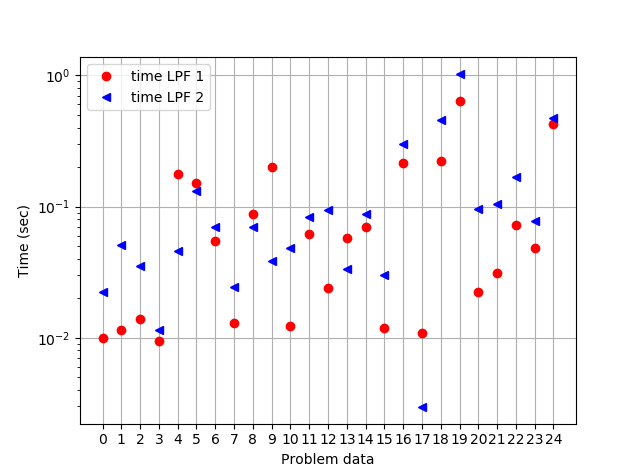
\includegraphics[width= 12 cm]{timeLPF12}\caption{Log plot time storage: test problems for comparing the two centering parameters.} 
\end{center}
\end{figure}
In Appendix A.3 are given the implementations of the LPF algorithm using $\sigma^{1}_{k}$, labelled as \textit{LPF 1}, and using $\sigma^{2}_{k}$, labelled as \textit{LPF 1}. The performance of them in term of number of iterations is reported in Section 4.6 together with the other interior-point algorithms under study.\\ The codes are well suited for this
purpose of comparison since the body (structure) of the code is the same for both algorithms. In Figure 4.2 we can give results about the speed of implementation of LPF 1 and LPF 2. The LPF with the centering parameter (\ref{LPF1}) requires more time storage then the one with (\ref{LPF2}) to find a LP solution for almost all problems, indipendently to the characteristic of the problem data. \newpage
From these excellent theoretical properties, it is designed a modified LPF algorithm: it exploits the fact that all iterates belong to $\mathcal{N}_{-\infty}(\gamma,\beta)$ of the central path but, with techniques presented in the next section, it may accelerate its performance. 


\section{Predictor-corrector algorithms}\label{sec:pc}
In the late 80s, Mehrotra and indipendently Lustig, Marsten, Shanno and their collaborators made impressive progress in the implementation of IPMs \cite{Mehr}. Two particular techniques have proved particulary successful in accelerating the IPM convergence: Mehrotra's predictor-corrector algorithm and multiple centrality correctors. \\Since these two procedures were designed, there have been a number of attempts to investigate their behaviour rigorosly but they are hard to analyse theoretically \cite{25y}, even if they are successful in practice: in fact several powerful methods are based on a variant of Mehrotra's algorithm.\\
%Most interior-point software written since 1990s have been based on Mehrotra's predictor-corrector algorithm (MPC).\\
%Since Karmarkar's landmark paper \cite{Kar}, IPM became one of the most active research area that produced a large amount of research results. Moreover, . \\
The Mehrotra's contribution was to combine the work developed by Montiero, Adles and Resende \cite{MARE} and the infeasible-interior-point path-following approach implemented by Lustig, Marsten and Shanno \cite{LMS}. 
The method incorporates these algorithmic devices that contribute to its practical success, including the use of different step lengths for the primal and dual variables and a heuristic choice of the step lengths that leads to speed the asymptotic convergence.\\In the research we will present a predictor-corrector LPF algorithm that is based on Mehrotra's approachdescribed in the following section. 
\subsection{Mehrotra's method}
We begin delineating a single iteration of the algorithm. It is not quite the same as the original algorithm from \cite{MER} but it is similar to the variant that is implemented in codes such as LIPSOL, LOQO and PCx (see Chapter 11 of \cite{Wright}): through this thesis we label simply as Mehrotra's method (MPC).\\
It generates sequence of infeasible iterates $\{(x^{k},\lambda^{k},s^{k})\}$ for which $(x^{k},s^{k})>0$. The search direction at each iteration consists of three components:
\begin{enumerate}
	\item an affine-scaling "predictor" direction;
	\item a centering term whose size is governed by the adaptively chosen centering parameter $\sigma$;
	\item a "corrector" direction that attempts to compensate for some of the nonlinearity in the affine-scaling direction.
	\end{enumerate}
The affine-scaling component is calculated before the centering component; by arranging the computations in this way, we gain a key advantage: the ability to choose the centering parameter $\sigma$ adaptively rather then a priori, as we did in the LPF algorithms.\\
If the affine-scaling direction makes good progress in reducing the duality measure $\mu$, while remaining inside the positive hyperplane defined by $(x,s)>0$, we conclude that little centering is needed, so we choose $\sigma$ close to 0. Otherwise, we can move only short distance along the affine-scaling direction before violating the positivity constraints, thus we need a significant amount of centering and $\sigma$ must be closer to 1.\\
Given a general LP problem (\ref{(Prim)}) MPC operates as follows. First af all, requiring the current point $(x, \lambda, s)$ satisfies only $(x, s)> 0$, we compute the affine-scaling directionas follows
\begin{equation}\label{(A)}\tag{4.21}
\begin{bmatrix}
0&A^{T}&I \\A&0&0\\S&0&X
\end{bmatrix}\begin{bmatrix}
\Delta x^{\text{aff}}\\\Delta\lambda^{\text{aff}}\\\Delta s^{\text{aff}}
\end{bmatrix}=-\begin{bmatrix}
r_{c}\\r_{b}\\XSe
\end{bmatrix}.
\end{equation}
Now we find the step lengths to the boundary along this direction, performing separate calculations for the primal and dual components reported below:
\begin{align}\label{Qw}\tag{4.22a}
\alpha_{\text{aff}}^{\text{pri}}=\arg\max\{\alpha\in[0,1]\;|\;x +\alpha\Delta x^{\text{aff}}\geq 0\}, \\
\alpha_{\text{aff}}^{\text{dual}}=\arg\max\{\alpha\in[0,1]\;|\;s +\alpha\Delta s^{\text{aff}}\geq 0\}\tag{4.22b}.
\end{align}
To measure the efficacy of the affine-scaling direction, it is defined $\mu_{\text{aff}}$ as the hypothetical value of $\mu$ resulting from a full step to the boundary, that is,
\begin{equation}\tag{4.22c}
	\mu_{\text{aff}}= (x+\alpha_{\text{aff}}^{\text{pri}}\Delta x^{\text{aff}})^{T}(s+\alpha_{\text{aff}}^{\text{dual}}\Delta s^{\text{aff}})/n.
\end{equation}
If $\mu_{\text{aff}}\ll\mu$, the affine-scaling direction is a good search direction that permits significant progress to be made in reducing $\mu$, so we choose the centering parameter $\sigma$ close to 0. Instead, if $\mu_{\text{aff}}$ is just a little smaller than $\mu$, we compute a bigger $\sigma$. The latter choice has the effect of moving us closer  to the central path $\mathcal{C}$, so that the algorithm is in a better position to achieve a substantial decrease in $\mu$ on the next iteration.\\
Mehrotra suggests the following heuristic in \cite{MER}, which is effective in exhaustive computational testing:
\begin{equation*}\label{CP}
\sigma = \bigg(\frac{\mu_{\text{aff}}}{\mu}\bigg)^{3}.
\end{equation*}
The second step consists on computing centering vector solving a linear system with the same coefficient matrix as in (\ref{(A)}) but the right-hand side equal to $-[0, 0,\sigma\mu e]$: actually it is combined with the third step, corrector phase, as we see now.\\
To motivate the corrector step, we see how the $i^{th}$ pairwise product $x_{i}s_{i}$ is affected by a full step in the affine-scaling direction. In fact, from (\ref{(A)}) we observe that:
\begin{equation*}
(x_{i}+\Delta x_{i}^{\text{aff}})(s_{i}+\Delta s_{i}^{\text{aff}})= x_{i}s_{i}+ x_{i}\Delta s_{i}^{\text{aff}}+s_{i}\Delta x_{i}^{\text{aff}}+\Delta x_{i}^{\text{aff}}\Delta s_{i}^{\text{aff}} =\Delta x_{i}^{\text{aff}}\Delta s_{i}^{\text{aff}}.
\end{equation*}
Hence a full step is taken, the pairwise product $x_{i}s_{i}$ transforms to $\Delta x_{i}^{\text{aff}}\Delta s_{i}^{\text{aff}}$, instead of 0. The corrector component vector $(\Delta x^{\text{cor}}, \Delta \lambda^{\text{cor}}, \Delta s^{\text{cor}})$ tries to compensate for this deviation from linearity, modifying the search direction so that the pairwise products come closer to their target value to 0. This step satisfies the following system:
\begin{equation}\label{(B)}
\begin{bmatrix}
0&A^{T}&I \\A&0&0\\S&0&X
\end{bmatrix}\begin{bmatrix}
\Delta x^{\text{cor}}\\\Delta\lambda^{\text{cor}} \\\Delta s^{\text{cor}}
\end{bmatrix}=-\begin{bmatrix}
0\\0\\\Delta X^{\text{aff}}\Delta S^{\text{aff}}e
\end{bmatrix},
\end{equation}
where
$
\Delta X^{\text{aff}} = \text{diag}(\Delta x_{1}^{\text{aff}}, \Delta x_{2}^{\text{aff}},\dots,\Delta x_{n}^{\text{aff}})$ and $\Delta S^{\text{aff}} = \text{diag}(\Delta s_{1}^{\text{aff}}, \Delta s_{2}^{\text{aff}},\dots,\Delta s_{n}^{\text{aff}})$.\\
To assess the effect of the corrector component, we examine the pairwise product obtained from a full step along the combined affine-scaling and corrector direction. From (\ref{(B)}), we have:
\begin{equation*}
(x_{i}+\Delta x_{i}^{\text{aff}}+\Delta x_{i}^{\text{cor}})(s_{i}+\Delta s_{i}^{\text{aff}}+\Delta s_{i}^{\text{cor}})= \Delta x_{i}^{\text{aff}}\Delta s_{i}^{\text{cor}}+\Delta x_{i}^{\text{cor}}\Delta s_{i}^{\text{aff}}+\Delta x_{i}^{\text{cor}}\Delta s_{i}^{\text{cor}}.
\end{equation*}
This result yelds to a better reduction of the duality measure, in fact we report the following bounds (from Chapter 10 of \cite{Wright}):
\begin{equation*} 
\lVert(\Delta x^{\text{aff}},\Delta s^{\text{aff}}) \rVert_{2} = \mathcal{O}(\mu)\text{ and }\lVert(\Delta x^{\text{cor}},\Delta s^{\text{cor}}) \rVert_{2} = \mathcal{O}(\mu^{2}).
\end{equation*}
When the limiting matrix is singular, the corrector step may no longer be smaller in norm than the affine-scaling step, ideed, it is often larger. Even in this situation, the use of the corrector component usually enhances the overall efficiency of the algorithm in practice.\\
Since the centering and corrector components are obtained by solving linear system with the same coefficient matrix and they are indipendent each other, we merge them into a single direction by adding their corresponding right-hand sides and compute the combined direction. We obtain the combined centering-corrector step $(\Delta x^{\text{cc}}, \Delta \lambda^{\text{cc}}, \Delta s^{\text{cc}})$ solving the following system:
\begin{equation}\label{(C)}
\begin{bmatrix}
0&A^{T}&I \\A&0&0\\S&0&X
\end{bmatrix}\begin{bmatrix}
\Delta x^{\text{cc}}\\\Delta\lambda^{\text{cc}} \\\Delta s^{\text{cc}}
\end{bmatrix}=-\begin{bmatrix}
0\\0\\\Delta X^{\text{aff}}\Delta S^{\text{aff}}e - \sigma\mu e
\end{bmatrix}.
\end{equation}
Although we need to solve at each iteration two linear systems instead of one, the marginal cost is not great because the systems have the same coeffifient matrix and then we need only modify the right-hand side. \\
Once the predictor and corrector terms are computed they are added to produce the final search direction
\begin{align*}
(\Delta x^{k},\Delta \lambda^{k},\Delta s^{k})=(\Delta x^{\text{aff}},\Delta \lambda^{\text{aff}},\Delta s^{\text{aff}})+(\Delta x^{cc},\Delta  \lambda^{cc},\Delta s^{cc})
\end{align*}
 Having described the essential elements of the method's approach, the algorithm is structured as follows:
\begin{algorithm}[H]\caption{Mehrotra's algorithm}
\begin{tabbing}
	\\
	\textbf{Given} $(x^{0}, \lambda^{0}, s^{0})$ with $(x^{0}, s^{0})> 0$ ; \\
	\textbf{for} \= $k = 0, 1, 2,...$ \\
	\> solve (\ref{(A)}) for $(\Delta x^{\text{aff}},\Delta \lambda^{\text{aff}},\Delta s^{\text{aff}})$;\\
	\> calculate $\alpha_{\text{aff}}^{\text{pri}}$, $\alpha_{\text{aff}}^{\text{dual}}$ and $\mu_{\text{aff}}$ as in (4.22);\\
	\> set centering parameter to $\sigma = (\mu_{\text{aff}}/\mu)^{3}$; \\
	\> solve (\ref{(C)}) for $(\Delta x^{cc},\Delta \lambda^{cc},\Delta s^{cc})$;\\
	\> compute the search direction and step to boundary from: \\
	\> \\
	\> $\;\;\;\;\;\;\;(\Delta x^{k},\Delta \lambda^{k},\Delta s^{k})=(\Delta x^{\text{aff}},\Delta \lambda^{\text{aff}},\Delta s^{\text{aff}})+(\Delta x^{cc},\Delta  \lambda^{cc},\Delta s^{cc})$;\\
	\> $\;\;\;\;\;\;\;\alpha_{\text{max}}^{\text{pri}}=\arg\max\{\alpha\geq0\;|\;x^{k} +\alpha\Delta x^{k}\geq 0\}$;\\
	\> $\;\;\;\;\;\;\;\alpha_{\text{max}}^{\text{dual}}=\arg\max\{\alpha\geq0\;|\;s^{k} +\alpha\Delta s^{k}\geq 0\}$;\\
	\>\\
	\> set $\alpha_{k}^{\text{pri}}=\min\{0.99\ast\alpha_{\text{max}}^{\text{pri}},1\}$;\\
	\> set $\alpha_{k}^{\text{dual}}=\min\{0.99\ast\alpha_{\text{max}}^{\text{dual}},1\}$;\\
	\> set\\
	\> $\;\;\;\;\;\;x^{k+1} = x^{k} + \alpha_{k}^{\text{pri}}\Delta x^{k}$;\\
	\>$\;\;\;\;\;\;(\lambda^{k+1},s^{k+1}) = (\lambda^{k},s^{k}) + \alpha_{k}^{\text{dual}}\Delta (\lambda^{k},\Delta s^{k})$;\\
\textbf{end}
\end{tabbing}
\end{algorithm}
It is worth noting that here it needed two step length parameters $\alpha_{k}^{\text{pri}$ and $\alpha_{k}^{\text{dual}$ instead of only one per iteration in the long-path following algorithms.
\newpage
\subsection*{Analysis of MPC}
In order to study the performance of the Mehrotra's algorithm, we introduce the trajectory-following methods from ODEs. These one define a trajectory from the current point, we say $(x,\lambda,s)$, to the solution $(x^{*},\lambda^{*},s^{*})$. There are infinitely many trajectories to choose from, but in this case it is obtained from a linear scaling of the function (\ref{F}).\\ Denoting this trajectory by $\mathcal{H}$ and parametrizing it by $\tau\in[0,1)$, we find that each point $(\hat{x},\hat{\lambda},\hat{s})_{\tau}\in\mathcal{H}$ is a solution of the following nonlinear system:
\begin{equation}\label{T}
\begin{bmatrix}
A^{T}\hat{\lambda}+\hat{s}-c \\A\hat{x}-b \\\hat{X}\hat{S}e
\end{bmatrix}=\begin{bmatrix}
(1-\tau)r_{c}\\(1-\tau)r_{b}\\(1-\tau)XSe
\end{bmatrix}, (\hat{x},\hat{s})\geq0,
\end{equation}
with $r_{c}$ and $r_{b}$ residuals respect to the initial point. We see that $(\hat{x},\hat{\lambda},\hat{s})_{\tau}$ with $\tau = 0$ is exactly the initial point and that $\lim\limits_{\tau\to1}(\hat{x},\hat{\lambda},\hat{s})_{\tau} = (x^{*},\lambda^{*},s^{*})$, if the limit exists.\\
To move along the trajectory $\mathcal{H}$, we can formulate a Taylor series approximation to $(\hat{x},\hat{\lambda},\hat{s})_{\tau}$ by expanding about the initial point  $(x,\lambda,s)$ as follows:
\begin{equation*}
(\hat{x},\hat{\lambda},\hat{s})_{\tau}=(\hat{x},\hat{\lambda},\hat{s})_{0}+\tau(\hat{x}^{'},\hat{\lambda}^{'},\hat{s}^{'})_{0}+\frac{1}{2}\tau^{2}(\hat{x}^{"},\hat{\lambda}^{"},\hat{s}^{"})_{0}+\dots = \sum_{j=0}^{\infty}\frac{\tau^{j}}{j!}(x^{j},\lambda^{j},s^{j})_{0}.
\end{equation*}
Here, $(\hat{x}^{j},\hat{\lambda}^{j},\hat{s}^{j})_{0}$ is the derivative of $(x,\lambda,s)_{\tau}$ with respect to $\tau$, evaluated in $\tau = 0$. We can find these derivatives by implicity differentiating (\ref{T}). Setting $\tau=0$, we have:
\begin{equation*}
\begin{bmatrix}
0&A^{T}&I \\A&0&0\\S&0&X
\end{bmatrix}\begin{bmatrix}
x_{0}^{'}\\\lambda_{0}^{'}\\s_{0}^{'}
\end{bmatrix}=-\begin{bmatrix}
r_{c}\\r_{b}\\XSe
\end{bmatrix},
\end{equation*}
which is exactly the same system as (\ref{(5.1)}).\\
Hence, we can identify $(\Delta x^{\text{aff}},\Delta \lambda^{\text{aff}},\Delta s^{\text{aff}})$ as $(x^{'}_{0},\lambda^{'}_{0},s^{'}_{0})$. Differentiating again with respect to $\tau$, we obtain the second derivative solving
\begin{equation*}
\begin{bmatrix}
0&A^{T}&I \\A&0&0\\\hat{X}_{0}&0&\hat{S}_{0}
\end{bmatrix}\begin{bmatrix}
x_{0}^{''}\\\lambda_{0}^{''}\\s_{0}^{''}
\end{bmatrix}=-\begin{bmatrix}
0\\0\\2X^{'}_{0}S^{'}_{0}e.
\end{bmatrix}
\end{equation*}
Instead here we see that $(\Delta x^{\text{cor}},\Delta \lambda^{\text{cor}},\Delta s^{\text{cor}})=\frac{1}{2}(x^{''}_{0},\lambda^{''}_{0},s^{''}_{0})$. Now we truncate the Taylor series at two terms and use the last two results, in order to have the following approximation:
\begin{equation*}
(\hat{x},\hat{\lambda},\hat{s})_{\tau}\approx(x, \lambda, s)+ \tau(\Delta x^{\text{aff}},\Delta \lambda^{\text{aff}},\Delta s^{\text{aff}})+\tau^{2}(\Delta x^{\text{cor}},\Delta \lambda^{\text{cor}},\Delta s^{\text{cor}}).
\end{equation*}
Now let us compare this approximation to the Mehrotra's iteration: ignoring the centering term by setting $\sigma =0$, if we constrain the primal and dual step lengths to be identical, we see in the algorithm the successive point will be
\begin{equation}
(\hat{x},\hat{\lambda},\hat{s})_{\tau}\approx(x, \lambda, s)+ \tau(\Delta x^{\text{aff}},\Delta \lambda^{\text{aff}},\Delta s^{\text{aff}})+\tau(\Delta x^{\text{cor}},\Delta \lambda^{\text{cor}},\Delta s^{\text{cor}}),
\end{equation} 
in which the $\tau^{2}$ coefficient in the last term is replaced by $\tau$.\\ Alternately, when we account for the centering parameter, the correspondence between the derivatives of the trajectory and the MPC search direction no longer holds. \\
Then, the modified trajectory $\mathcal{H}_{\sigma}$ is introduced for which the correspondence delineated above holds even in the presence of $\sigma$. Also $\mathcal{H}_{\sigma}$ starts at $(x, \lambda, s)$ and aims at the solution $(x^{*},\lambda^{*},s^{*})$ and all $(\hat{x},\hat{\lambda},\hat{s})_{\tau}$ in this trajectory satisfy:
\begin{equation}\label{Tt}
\begin{bmatrix}
A^{T}\lambda+s-c \\Ax-b \\XSe
\end{bmatrix}=\begin{bmatrix}
(1-\tau)r_{c}\\(1-\tau)r_{b}\\(1-\tau)XSe+\tau^{2}(1-\tau)\sigma\mu e
\end{bmatrix},(x,s)\geq0.
\end{equation}
The tangent to this trajectory is the affine-scaling direction, as for $\mathcal{H}$, but the curvature can be identified with the combined centering-corrector step rather than the corrector component alone. The trajectory $\mathcal{H}_{\sigma}$ approximates more the central path than $\mathcal{H}$. Despite the closer relationship between $\mathcal{H}_{\sigma}$  and MPC algorithm, we can not qualify it as a second-order trajectory-following algorithm because it still searches along a linear direction rather than a quadratic path.\\
The Newton step produced by MPC algorithm can be interpreted as a perturbed composite Newton method \cite{Col} and Tapia, Zhang and Dennys gave results on the order of convergence \cite{Topia}. Under additional assumption such as feasibility of the initial point, strict complementary and nondegeneracy of the $\epsilon$-solution the Mehrotra's method has cubic convergence. But in a recent study in \cite{Carta} it is provided a redable example that Mehrotra's technique may produce a correcotr which is larger in magnitude than the predictor and points in the wrong direction, possibly causing the algorithm to fail.
\\In the numerical testing we will see that the implementation yields excellent results in vast majority of cases. 
\subsection{A predictor-corrector LPF method}
As we have already mentioned, predictor-corrector methods are among the most effcient IPMs and have became the back bones of several optimization packages.\\
In this section it is constructed a long-path following method in which the centering parameter $\sigma$ is computed adaptively, using the Mehrotra's approach.\\
This algorithm  (PC LPF), illustrated below, is a definite improvement over the long-path following algorithm due to the adaptivity that is built adding a predictor step. We will discuss if eventually this potential
technique may further accelerate the performance obtained by the LPF methods outlined previously.\\

We have applied the adaptivity strategy as well. Let suppose we have computed the $k^{th}$ iterate, then we compute the affine-scaling direction: with $(\Delta x^{\text{aff}},\Delta \lambda^{\text{aff}},\Delta s^{\text{aff}})$ the following predictor step length $\alpha_{\text{aff}}^{\text{pre}}$ is necessary to measure $\mu_{\text{aff}}$, as following:
\begin{align}
\alpha_{\text{aff}}^{\text{pre}}&=\arg\max\{\alpha\in[0,1]\;|\;(x^{k}, \lambda^{k}, s^{k})+ \alpha(\Delta x^{\text{aff}}, \Delta\lambda^{\text{aff}}, \Delta s^{\text{aff}})\in\mathcal{N}_{-\infty}(\gamma,\beta)\}\label{QWw}\\
\mu_{\text{aff}}&= (x+\alpha_{\text{aff}}^{\text{pri}}\Delta x^{\text{aff}})^{T}(s+\alpha_{\text{aff}}^{\text{dual}}\Delta s^{\text{aff}})/n.\label{QWz}
\end{align}
in which $\mu_{\text{aff}}$ measures the efficiency of the affine-scaling direction, like in predictor step of MPC algorithm.
Then, the corrector step consists on solving the general linear system with the centering parameter equal to \begin{center*}
$\sigma_{k} = (\mu_{\text{aff}}/\mu)^{3}$, as in MPC. The value of the step length is performed in order to guarantee that the next iterate $(x^{k+1}, \lambda^{k+1}, s^{k+1})\in\mathcal{N}_{-\infty}(\gamma,\beta)$ and, as we have already noticed, the step length selection is different from the one in the MPC.\\The LPF variant is completely described by the following pseudocode.
\end{center*}\\
\begin{algorithm}[H]\caption{\label{alg:pc}PC LPF Algorithm}
	\begin{tabbing}
		\\
		\textbf{Given} $(x^{0}, \lambda^{0}, s^{0})$ with $(x^{0}, s^{0})> 0$; \\
		\textbf{for} \= $k = 0, 1, 2,...$ \\
		\> solve (\ref{(A)}) for $(\Delta x^{\text{aff}},\Delta \lambda^{\text{aff}},\Delta s^{\text{aff}})$;\\
		\> calculate $\alpha_{\text{pre}}^{\text{aff}}$ and $\mu_{\text{aff}}$ as in ($\ref{QWw}$) and in (\ref{QWz});\\
		\> set centering parameter to $\sigma_{k} = (\mu_{\text{aff}}/\mu)^{3}$; \\
		\> solve (\ref{Pb}) for $(\Delta x^{k},\Delta \lambda^{k},\Delta s^{k})$;\\
		\> choose the largest value in $\alpha_{k}\in[0,1]$ so that $(x^{k+1}, \lambda^{k+1}, s^{k+1})\in\mathcal{N}_{-\infty}(\gamma,\beta)$;\\
		\textbf{end}
	\end{tabbing}
\end{algorithm}
The goal of this algorithm is to take advantage of the neighborhood and the predictor-corrector strategy: the success of the algorithm is seen in the next chapter but it is interesting observing that $\mathcal{N}_{-\infty}(\gamma,\beta)$ limits the predictor-corrector's feature.
\newpage
\section{IPM algorithms performance}
In this section we develop an empirical study of the IPM algorithms performace, comparing the proposed methods with the implementations reported in Appendix A. \\
Given a general LP, we rate the number of iterations $T$ required to solve it to the number of constraints $m$ and the number of variables $n$. We may assume that $T$ can be approximated by a function of the form 
\begin{equation*}
	T \approx 2^{\alpha}(m+n)^{\beta},
\end{equation*}
for a pair of real numbers $\alpha$ and $\beta$. This multiplicative representation of the numbers of iterations can be converted into an additive representation by taking logarithms. Introducing an $\epsilon$ to value the difference between the model's prediction and the true number of iterations, we see that the model can be written as
\begin{equation*}
\log T \approx \alpha \log 2 +\beta \log (m+n) +\epsilon.
\end{equation*}
Now we compute $T$ related to the IPM methods proposed in this thesis: long-path following algorithms with centering parameter $\sigma_{k}^{1}$ and with $\sigma_{k}^{2}$ formulated respctively in (\ref{LPF1}) and in (\ref{LPF2}), PC LPF and Mehrotra's algorithms. In order to find $\alpha$ and $\beta$  for each method, we introduce the following regression model, with $k$ observations:\\
\begin{equation}
\begin{bmatrix}
\log T_{1}\\\log T_{2}\\\dots\\\log T_{k}\\
\end{bmatrix}
 =
 \begin{bmatrix}
\log 2&\log (m_{1}+n_{1})\\
\dots&\dots\\
\log 2&\log (m_{k}+n_{k})
\end{bmatrix}\begin{bmatrix}
\alpha\\\beta
\end{bmatrix}
+
\begin{bmatrix}
\epsilon_{1}\\
\dots\\
\epsilon_{k}
\end{bmatrix}.
\end{equation}
We test the algorithms on 30 small scale LP problems in standard form with model data $A\in\mathbb{R}^{m,n}$, $b\in\mathbb{R}^{m}$ and $c\in\mathbb{R}^{n}$. In Table \ref{tab:numite} the statistics from the runs is collected, summarizing the number of iterations $T_{k}$ required to solve the $k^{th}$ example, with $k =1,\dots,30$.
\begin{table}\caption{\label{tab:numite}Number of iterations required to solve standard LP problems with $n$ variables and $m$ constraints.}
	\begin{center}
	\begin{tabular}{cccccc}
		\hline
		\textbf{rows $m$} & \textbf{columns $n$} & \textbf{MPC $T_{k}$} & \textbf{PC LPF $T_{k}$} & \textbf{LPF 1 $T_{k}$} & \textbf{LPF 2 $T_{k}$} \\ \hline
		1 & 2 & 6 & 7 & 60 & 8 \\
		2 & 2 & 6 & 7 & 66 & 8 \\
		4 & 2 & 6 & 7 & 83 & 10 \\
		2 & 2 & 5 & 6 & 64 & 8 \\
		3 & 3 & 7 & 11 & 88 & 8 \\
		2 & 5 & 7 & 9 & 96 & 9 \\
		2 & 5 & 7 & 8 & 99 & 10 \\
		3 & 2 & 5 & 6 & 74 & 7 \\
		2 & 4 & 7 & 9 & 93 & 9 \\
		3 & 4 & 7 & 11 & 99 & 8 \\
		3 & 2 & 6 & 7 & 74 & 8 \\
		3 & 3 & 7 & 8 & 80 & 8 \\
		3 & 2 & 6 & 9 & 81 & 9 \\
		2 & 3 & 6 & 7 & 81 & 8 \\
		3 & 3 & 7 & 10 & 102 & 9 \\
		3 & 3 & 7 & 10 & 90 & 9 \\
		3 & 2 & 5 & 7 & 72 & 7 \\
		10 & 6 & 9 & 15 & 162 & 14 \\
		2 & 2 & 5 & 5 & 61 & 6 \\
		20 & 10 & 9 & 11 & 208 & 15 \\
		55 & 50 & 11 & 21 & 405 & 17 \\
		6 & 5 & 7 & 8 & 126 & 8 \\
		7 & 7 & 6 & 8 & 131 & 8 \\
		8 & 2 & 7 & 10 & 138 & 10 \\
		2 & 4 & 7 & 8 & 98 & 8 \\
		10 & 24 & 8 & 16 & 224 & 15 \\
		11 & 17 & 7 & 13 & 213 & 12 \\
		20 & 64 & 9 & 19 & 20 & 20 \\
		8 & 19 & 6 & 11 & 174 & 12 \\
		35 & 23 & 9 & 41 & 306 & 16 \\ \hline
	\end{tabular}
\end{center}
\end{table}
These performance profiles provide an estimate of the expected performance difference
between solvers.
\begin{figure}\label{figure:T}
	\begin{center}
		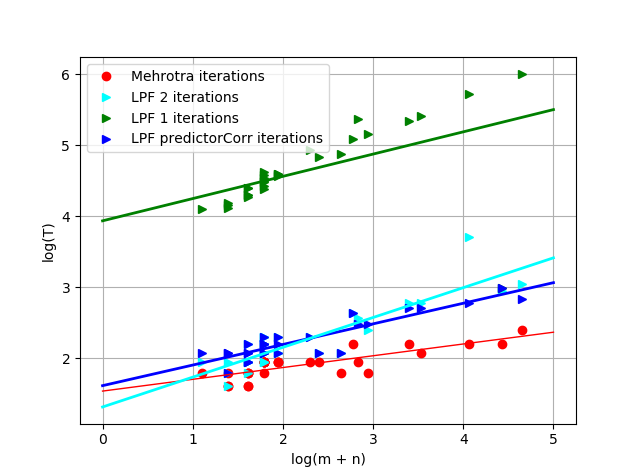
\includegraphics[width= 15 cm]{numberiterations}\caption{log–log plot of T vs. $m + n$ and the $L^{1}$ regression lines.}
	\end{center}
\end{figure}
%\ref{figure:T}
The Figure 4.2 shows a log-log plot of $T$ versus $m + n$ and the $L^{1}$ regression lines for all methods: we can conclude that the algorithm codes used in this research solve LP problems after T iterations approximated by
\begin{align*}
T& \approx 2^{0.1657}(m + n)^{1.5394} \text{ with Mehrotra's method,}\\
T &\approx 2^{0.313}(m + n)^{3.9349} \text{ with LPF1 method,}\\
T& \approx 2^{0.2898}(m + n)^{1.6157} \text{ with LPF2 method,}\\
T& \approx 2^{0.3955}(m + n)^{1.3784} \text{ with PC LPF method.}\\
\end{align*}
These outcomes confirm the practical success of the IPM, proving their polynomial complexity. Besides, it evinces the superiority of the Mehrotra's method. 
%\lstinputlisting[language=py,caption=applicationContext.py]{Forest.py}

%\begin{table}[]
%\begin{center}
%	\begin{tabular}{|l|l|}
%		\hline
%		{Example} & {\color[HTML]{333333} Convergence rate: K} \\ \hline
%		0 & 2.006 \\
%		1 & 5.537 \\
%		2 & 0.736 \\
%		3 & 3.152 \\
%		5 & 4.025 \\
%		6 & 7.115 \\
%		7 & 3.358 \\
%		8 & 7.208 \\
%		9 & 3.246 \\
%		10 & 1805.964 \\
%		11 & 5.712 \\
%		12 & 9.208 \\
%		13 & 14.010 \\
%		14 & 1.532 \\
%		17 & 6.714 \\
%		19 & 36.431 \\
%		21 & 24.663 \\
%		22 & 1237.766 \\
%		23 & 4.223  \\ \hline
%	\end{tabular}
%\end{center}
%\end{table}

\chapter{Implementation details}
We have implemented the algorithms; in each of them a sequence of primal-dual iterates $(x^{k},\lambda^{k},s^{k})$ is computed and at each $k^{th}$ iteration the duality measure $\mu_{k}$ is set.\\
Besides, in the problem tests it is traced also the absolute value of the duality gap $g$: we see it is important for the termination criteria and also gives informations about the infeasibiliy of the iterates. In fact, as we know, if $(x,\lambda,s) \notin \mathcal{F}$, then we have the residuals $r_{b}$ and $r_{c}$ not null, and: 
\begin{align*}
|g|=|c^{T}x-b^{T}\lambda|=|y^{T}Ax+s^{T}x-r_{c}^{T}x+r_{b}^{T}\lambda-x^{T}A^{T}\lambda|\geq |s^{T}x|.
\end{align*}
In this chapter we guide the reader through the issues and details of implementation of IPMs. As we have already seen, the general IPM code needs to initialise and terminate the algorithm in a reasonable way: we see several techniques which their effect in some numerical experiments are investigated in Chapter 6.  
\section*{Initialization and termination}
In the theoretical analysis of IPMs it is required the feasibility of the primal-dual starting point, hence $(x^{0}, \lambda^{0}, s^{0})\in\mathcal{F}^{0}$. Under theis assumption, the algorithms sequence begins in the interior of the feasible region and travel on
a path towards the the boundary, converging at the optimal solution. In practice there is no need to impose the feasibility of all iterates and force the algorithm to stay in the interior of the primal-dual feasible set $\mathcal{F}$.\\
It is already proved that IPMs are sensitive to the choice of an initial primal-dual point; in fact, "poor" starting points may drastically reduce the steps toward the solution, giving significant impact on the robustness of the algorithm. Therefore, the choice of good initial values is an important issue in the implementation of the methods. A common way to deal with it is to use heuristic-based strategies that try to keep the infeasibility small while ensuring that nonnegative variables are far enough from zero.\\
Since most of IPMs attempt to follow the central path $\mathcal{C}$, a very simple choice for the starting point would be to set the nonnegative variables to one and the others to zero. It is guaranteed that the point is perfectly centered, that is all pairwise complementarity products are equal to $\mu$ and the nonnegative variables are sufficiently bounded away from zero: $(x^{0},\lambda^{0},s^{0})=(e, 0, e)$, with $e$ and $0$ respectively unit and null vectors with appropriate dimensions. However, this point be far from satisfying the constraints \cite{VAN}.\\
Another strategy, that does not require the starting point is both well centerd and not too infeasible, is presented by Mehrotra \cite{MER}, that we will briefly call it as \textit{Mehrotra's initial point} method (MIP). This popular heuristic approach for finding $(x^{0}, \lambda^{0}, s^{0})$ consists on computing least squares solutions of the equations corresponding to the linear constraints of the LP and then shifting the values of the variables to ensure that they are kept away from their lower bound of zero. \\
The construction starts by calculating $(\tilde{x}, \tilde{\lambda}, \tilde{s})$ as solution of the two least-squares problems outlined below:
\begin{align*}
\min\limits_{x} \lVert x \rVert ^{2} &\text{ subject to }Ax = b,\\
\min\limits_{(\lambda,s)} \lVert s \rVert ^{2} &\text{ subject to } A^{T}\lambda +s = c,
\end{align*}
with $A$, $b$ and $c$ given from ($\ref{(Prim)}$). That is, $\tilde{x}$ and $\tilde{s}$ are the vectors of least norm that are in $\mathcal{F}$ and they are computed using the following formulas:
\begin{equation}\label{71}
\tilde{x} = A^{T}(AA^{T})^{-1}b,\;\;\;\tilde{\lambda}=(AA^{T})^{-1}Ac,\;\;\; \tilde{s} = c- A^{T}\tilde{\lambda}.
\end{equation}
Since in general $\tilde{x}$ and $\tilde{s}$ are not positive, we compute
\begin{equation*}
\delta_{x} = \max\{-(3/2)\min\limits_{i}\tilde{x}_{i},0\},\;\;\; \delta_{s} = \max\{-(3/2)\min\limits_{i}\tilde{s}_{i},0\},
\end{equation*}
to define the positive vectors $\hat{x}= \tilde{x}+\delta_{x}e$ and $\hat{s}= \tilde{s}+\delta_{s}e$, whit $e$ the unit vector. To ensure that the initial points $x^{0}$ and $s^{0}$ are not too close to zero, we add two more scalars defined as follows:
\begin{align}\label{72}
\tilde{\delta}_{x}= \frac{1}{2}\frac{\hat{x}^{T}\hat{s}}{e^{T}\hat{s}},\;\;\;\tilde{\delta}_{s} =\frac{1}{2}\frac{\hat{x}^{T}\hat{s}}{e^{T}\hat{x}}.
\end{align}
The starting point is then defined as 
\begin{align*}
(x^{0}, \lambda^{0}, s^{0}) = (\tilde{x}+\tilde{\delta}_{x} e,\;\tilde{\lambda},\;\tilde{s}+\tilde{\delta}_{s} e).
\end{align*}
\\
\begin{figure}\caption{\label{fig:MIP}Starting point strategy MIP.}
	\centering
	{\noindent\begin{boxedminipage}{1\linewidth}
			\begin{tabbing}
			compute \=$(\tilde{x},\tilde{\lambda},\tilde{s})$ as in (\ref{71});\\				
			\=\\
				\>$\bar{x} = \min\{x_{i}\}$;\\
				\>$\bar{s} = \min\{s_{i}\}$;\\
				\textbf{if} \= $\bar{x}<0$ then\\
				\> $\hat{x}= \tilde{x} -(3/2)\bar{x}e$;\\
				\textbf{else} \=\\
				\> $\hat{x} = \tilde{x}$\\
				\textbf{if} \= $\bar{s}<0$ then\\
				\> $\hat{s}= \tilde{s} -(3/2)\bar{s}e$;\\
				\textbf{else} \=\\
				\> $\hat{s} = \tilde{s}$;\\
				compute \=(\ref{72}) with $\hat{x}$ and $\hat{s}$\\
				\>$(x^{0}, \lambda^{0}, s^{0}) = (\tilde{x}+\tilde{\delta}_{x} e,\;\tilde{\lambda},\;\tilde{s}+\tilde{\delta}_{s} e)$\\
				\textbf{end}
			\end{tabbing}
		\end{boxedminipage}
		} \quad
\end{figure}
The logical basis of this strategy (stated in Figure \ref{fig:STP1}) is that many LPF methods are able to perform long steps toward the solution and to drive the infeasibility to zero at least at the same rate as the duality gap, by keeping the iterates in the neighbourhood $\mathcal{N}_{-\infty}(\gamma,\beta)$, defined in (\ref{neigh3}) \cite{SPS}.\\[1 cm]
The second starting-point strategy is suggested by the convergence theory of the Potential Reduction method \cite{SPS}. The starting point can be chosen as \begin{equation*}
(x^{0}, \lambda^{0}, s^{0}) = \eta \tilde{w},
\end{equation*}where $\tilde{w} = (e,0,e)$ and $\eta$ is the value such that the residuals $r_{b}^{0}$ and $r_{c}^{0}$ and the duality measure $\mu_{0}$ corresponding to this starting point satisfy the following:

\begin{equation}\label{su}
\frac{\lVert(r^{0}_{b},r^{0}_{c})\rVert_{2}}{\mu_{0}}\leq \tau<1. 
\end{equation}
It easy to verify that, since $\mu_{0}$ increases quadratically and $\lVert(r^{0}_{b},r^{0}_{c})\rVert_{2}$ increases linearly with $\eta$, the inequality (\ref{su}) approximately holds if $\eta$ satisfies
\begin{equation*}
\eta\geq \frac{\lVert(\tilde{r}_{b},\tilde{r}_{c})\rVert_{2}}{\tau\tilde{\mu}},
\end{equation*}
where $\lVert(\tilde{r}_{b},\tilde{r}_{c})\rVert_{2}$ and $\tilde{\mu}$ are respectively the infeasibility error norm and the duality measure associated with $\tilde{w}$ (in this case $\tilde{\mu} = n$). \\
We notice that $(x^{0},\lambda^{0},s^{0})$ is perfectly centered and all its components with lower bound 0 are "sufficient" positive, but even if the ratio in (\ref{su}) is small, the duality gap and the infeasibility may very large, slowing the progress toward the solution.\\
This method strategy, to which we will refer STP, is summarized in the Figure \ref{fig:STP2}.\\
\begin{figure}\caption{\label{fig:STP2}Starting point strategy STP.}
	\centering
	{\noindent\begin{boxedminipage}{1\linewidth}
			\begin{tabbing}
			$\;$choose $\tau < 1$;  \\
			$\;\tilde{w}=(e,0,e)$;\\
			$\;\tilde{\sigma}= \lVert\tilde{r}_{b},\tilde{r}_{c})\rVert_{2}$;\\
			$\;\tilde{\mu}= n$;\\
			\textbf{ If} \= $\tilde{\sigma}/n\leq \tau$ then\\
			\> $(x^{0}, \lambda^{0}, s^{0}) = \tilde{w}$;$\;\;\;\;\;\;$\\
			\textbf{ else}\>\\
			\> $\tilde{\mu}=\tilde{\sigma}/(\tau n)$; \\
            \> $(x^{0}, \lambda^{0}, s^{0}) = \eta \tilde{w}$;\tab \\
			\textbf{ end}
			\end{tabbing}
\end{boxedminipage}
} \quad
\end{figure}

%Now we obtain the infeasibility error norms and the duality gaps corresponding to the starting points computed with MIP and STP for small size LP problems.\\
\begin{table}[!h]\caption{\label{fig:STP1} Analysis of the starting-point strategies.}	
	\begin{tabular}{llllllllll}
		\hline
		\textbf{Size} &  &  & \textbf{MIP}&&  &  & \multicolumn{3}{l}{\textbf{      STP}} \\ \cline{1-2} \cline{4-6} \cline{8-10} 
		m & n &  & infeasibility & duality measure & ratio &  & infeasibility & duality measure & ratio \\ \hline
		1 & 2 &  & 2.07e+01 & -1.98e-01 & -104.65 &  & 2.73e+01 & -1.12e+00 & -2.43e+01 \\
%		2 & 2 &  & 8.05e+00 & 6.25e-01 & 12.87 &  & 9.17e+00 & 9.71e-01 & 9.45e+00 \\
		4 & 2 &  & 5.39e+03 & 2.32e+03 & 2.32 &  & 1.65e+04 & 8.90e+03 & 1.85e+00 \\
%		2 & 2 &  & 5.19e+01 & 1.62e+01 & 3.21 &  & 9.20e+01 & 4.33e+01 & 2.12e+00 \\
%		2 & 2 &  & 6.04e+01 & 4.41e+00 & 13.70 &  & 1.20e+01 & 9.62e-01 & 1.25e+01 \\
		3 & 3 &  & 4.30e+01 & 6.72e+00 & 6.40 &  & 1.93e+02 & 3.05e+01 & 6.32e+00 \\
		2 & 5 &  & 4.73e+01 & 1.46e+00 & 32.31 &  & 9.88e+00 & 1.64e+00 & 6.02e+00 \\
		2 & 5 &  & 3.60e+01 & -3.93e+01 & -0.92 &  & 1.34e+02 & -1.53e+02 & -8.73e-01 \\
		3 & 2 &  & 5.66e+00 & 4.41e-01 & 12.82 &  & 3.61e+00 & 4.00e-01 & 9.01e+00 \\
		2 & 4 &  & 1.11e+02 & -2.14e+01 & -5.20 &  & 1.16e+02 & -4.26e+01 & -2.73e+00 \\
%		3 & 4 &  & 3.11e+01 & -5.69e+00 & -5.46 &  & 1.28e+04 & -2.86e+03 & -4.46e+00 \\
		3 & 2 &  & 1.09e+01 & 1.05e+00 & 10.36 &  & 1.02e+02 & 1.02e+01 & 9.97e+00 \\
		3 & 3 &  & 1.86e+01 & 2.52e+00 & 7.38 &  & 2.90e+01 & 5.44e+00 & 5.33e+00 \\
		3 & 2 &  & 5.09e+01 & 1.07e+01 & 4.74 &  & 1.10e+01 & 3.33e+00 & 3.30e+00 \\
		2 & 3 &  & 3.25e+01 & -2.11e+00 & -15.37 &  & 9.92e+00 & -1.95e+00 & -5.09e+00 \\
%		3 & 3 &  & 2.74e+01 & -2.78e+00 & -9.83 &  & 5.82e+00 & -1.58e+00 & -3.69e+00 \\
		3 & 3 &  & 5.90e+01 & 6.51e+00 & 9.07 &  & 3.21e+01 & 4.16e+00 & 7.72e+00 \\
		3 & 2 &  & 1.44e+01 & 3.38e+00 & 4.25 &  & 3.55e+01 & 1.18e+01 & 3.01e+00 \\
		10 & 6 &  & 9.23e+03 & 1.08e+04 & 0.86 &  & 6.43e+04 & 9.45e+04 & 6.80e-01 \\
		2 & 2 &  & 3.33e+01 & 5.88e-01 & 56.57 &  & 3.97e+01 & 8.77e-01 & 4.53e+01 \\
%		2 & 2 &  & 3.49e+01 & 2.42e+01 & 1.44 &  & 3.13e+01 & 3.22e+01 & 9.71e-01 \\
		20 & 10 &  & 7.46e+04 & 1.65e+04 & 4.51 &  & 8.09e+05 & 1.80e+05 & 4.50e+00 \\
		55 & 50 &  & 1.15e+04 & 2.07e+02 & 55.81 &  & 6.71e+05 & 6.24e+04 & 1.08e+01 \\
		4 & 8 &  & 6.14e+01 & -2.72e+00 & -22.57 &  & 1.50e+01 & -5.48e+00 & -2.74e+00 \\
		6 & 5 &  & 1.81e+01 & -5.88e-01 & -30.79 &  & 4.06e+00 & -2.73e-01 & -1.49e+01 \\
		13 & 6 &  & 1.18e+04 & 1.41e+05 & 0.08 &  & 5.20e+03 & 1.05e+05 & 4.94e-02 \\
		7 & 7 &  & 5.86e+01 & -2.77e+00 & -21.17 &  & 1.05e+01 & -5.00e-01 & -2.11e+01 \\
		8 & 2 &  & 8.30e+01 & -5.62e+00 & -14.76 &  & 5.37e+01 & -5.07e+00 & -1.06e+01 \\
		2 & 4 &  & 2.64e+01 & -6.25e+00 & -4.22 &  & 2.58e+01 & -1.21e+01 & -2.13e+00 \\
		10 & 24 &  & 1.49e+05 & -1.70e+04 & -8.78 &  & 2.77e+09 & -3.15e+08 & -8.77e+00 \\ \hline
	\end{tabular}\caption{Infeasibility equal to $\lVert (r_{b}, r_{c})\rVert_{2}$, duality measure ${\mu}$ and their ratios corresponding to the initial points obtained with MIP and STP1.}
\end{table}
Now we compare the two strategies testing them on 30 small size LP problems.\\ 
We check whether the strategies aim at satisfying the requirement that the starting point is both "well centerd" and "not too infeasible". It is reported the numerical results in Table \ref{fig:STP1} and it is confirmed that it is not a evident peculiar behaviour of the infeasibility error and the duality measure obtained by each strategy. Even if the ratios are smaller for the STP initial points, the duality measure and the infeasibility error are competitive and they don't lead to an effective comparison. \\Eventually, we can't a priori determine the best initial values, but we will see in the numerical tests developed in Chapter 6 that it is worth distinguish the two cases corresponding to the two strategies adopted in the IPMs codes. 
\newpage
Now we deal on the termination criteria; unlike the simplex method, interior-point algorithms never find an exact solution of the LP.\\ All the algorithms studied in this research have in common a finite termination phase that reports an approximate solution for which the residuals $r_{b}$ and $r_{c}$ and the duality gap $g$ are sufficiently small. After determinated a small tollerance $\epsilon$, the algorithms terminate when the following conditions on the relative primal and dual residuals and the relative duality gap are satisfied:
\begin{align}\label{TermC}
\frac{\lVert r_{b}\rVert_{2}}{1+ \lVert b \rVert_{2}}\leq \epsilon, && \frac{\lVert r_{c}\rVert_{2}}{1 + \lVert c \rVert_{2}}\leq \epsilon, &&\frac{|g|}{1+b^{T}y}\leq \epsilon,
\end{align}
The tollerance value $\epsilon > 0$ is usually of the order $10^{-8}$, as required both in the literature and in practice \cite{Wright}. It is rare that the third condition is satisfied and at the same time
other conditions do not hold; consequently, the most important and perhaps
the only condition that really has to be checked is the third condition \cite{ADL}.\\
That is confirmed across the obtained numerical results stated in Chapter 6: reporting the behaviour of $g$ and $\lVert r_{b},r_{c}\rVert_{2}$, it occurs that the first moves slower than the second value in the iterations to the tollerance $\epsilon$.\\
\section*{Solving the linear system}
We focus on the core linear algebra operation in primal-dual IPMs: the solution of the linear equations system (\ref{(5.1)})
whose coefficient matrix has dimension $(2n+m)\times(2n+m)$ and it displays a sparsity pattern, because of the presence of several zero blocks and diagonal matrices.\\In existing codes, the linear
system is formulated in two different ways which we now outline; let us consider the matrix (\ref{matrix:LPF}), that incorporates the affine method's matrix just getting $\sigma=0$.
Now we formulate it with a new more compact symmetric coefficient matrix, which
is easier and cheaper to factor than the original form. Since the current point $(x, \lambda, s)$ has $x$ and $s$ strictly
positive, the diagonal matrices $X$ and $S$ are nonsingular; hence, by eliminating $\Delta s$, we obtain the following equivalent system, called \textit{augmented system}:
\begin{align*}
\begin{bmatrix}
0&A\\A^{T}&-D^{2}
\end{bmatrix}\begin{bmatrix}
\Delta\lambda \\\Delta x
\end{bmatrix}=&-\begin{bmatrix}
r_{c}\\r_{b} + \sigma\mu(X)^{-1}e
\end{bmatrix},\\
\Delta s =& -s +\sigma\mu (X)^{-1}S\Delta x,
\end{align*}
where we have introduced the notation $D = S^{-1/2}X^{1/2}$.\\
Since the matrix $X^{-1}S$ is also diagonal and nonsingular, we can eliminate $\Delta x$ from the first row of the augmented system to obtain another equaivalent form:
\begin{align*}
AD^{2}A^{T}\Delta\lambda &= -r_{b}+A(-S^{-1}Xr_{c}+ x - \sigma\mu S^{-1}e),\\
\Delta s &= -r_{c}-A^{T}\Delta \lambda,\\
\Delta x &= -x + \sigma \mu S^{-1}e-S^{-1}X\Delta s.
\end{align*}
\\
This form often is called the \textit{normal equations} form and a direct sparse Cholesky algorithm is applied to factor the matrix $AD^{2}A^{T}$. \\Both forms are performed and ill-conditioning is often observed during the final steps of the LPF algorithms using the normal equations, because the elements of the diagonal weighting
matrix $D^{2}$ take on both huge and tiny values.
Then, in the codes it is took in consideration only the second variant: from our observations the effort of the augmented system is not different respect to using (\ref{(5.1)}), except for the Mehrotra's algorithm in finding the solution of the ONB problem in Section 6.4. In fact, the whole system gives sparsity problems. 
\section*{Geometric point of view}
Now we outline the geometric viewpoint of the simplex method and the IPMs, assuming the LP problem is in standard form.\\
We have already stated that the simplex method generates a sequence of basic feasible primal points of the set $\mathcal{P}$, defined in (\ref{PP}). It picks a vertex of the polytope, then it checks its neighbours: if there is a neighbour that gives a
better solution with respect to the objective function, it pivots to that new vertex.
It repeats this procedure until the optimal solution is reached and none of its neighbouring vertices will give
a better solution.\\Instead, the primal-dual IPMs travel theoretically within the interior of the feasible set $\mathcal{F}$ to search for an optimal solution, generating the central path $\mathcal{C}$, rather than working around the boundary.\\ The main idea of the path-following methods is to follow $\mathcal{C}$ in the direction of decreasing $\tau$ in (4.3); actually they do not necessarily stay exactly on the path but within a loose and well-defined neighoborhood of $\mathcal{C}$ while steadily reducing the duality measure $\mu$ to zero. Each search direction is computed with a Newton's step toward a point for which the duality measure $\tau$ is equal to or smaller than the current duality measure $\mu$, as we know $\tau=\sigma\mu$. \\
The affine-scaling method, based on pure Newton's steps, sets the central parameter $\sigma= 0$ in the system (\ref{Pb}) but its limit is that,
%In fact, the gap between neighborhood boundaries is wide enough to allow this step to make significant progress in reducing $\mu$. 
even if it makes significant progress at each iteration, it also tends to worsen the centrality measure (condition of having all pairwise products $x_{i}s_{i}$ equal). Therefore, the step length $\alpha$ is often really small, in order to garantee the next primal-dual point remains in $\mathcal{F}$; hence, the affine-scaling search direction does not allow us to make much progress toward a solution.\\ 
The long-path following method doesn't create a sequence that moves strongly to the solution, indeed, computes at the $k^{th}$ iteration the search direction with $\sigma_{k}$ between two fixed limits $\sigma_{\text{min}}$ and $\sigma_{\text{max}}$, in order to improve the centrality measure. The lower bound $\sigma_{\text{min}}$ ensures that each search direction start by moving off the boundary of $\mathcal{N}_{-\infty}(\gamma)$ and into the interior of the neighborhood. It is easy to prove that unit steps length along the search direction would take the next point outside the neighborhood, since the error of approximating the nonlinear KKT system by the linear equations becomes more pronounced as $\alpha$ increases. Then, it is selected $\alpha$ as large a possible subject to the next point remains $\mathcal{N}_{-\infty}(\gamma)$. In the LPF implementations we set $\sigma_{\text{min}}=0$ and $\sigma_{\text{max}}=1$: this restriction achieves the twin goals of improving centrality and reducing the duality measure into a single step.\\
Alternatively, the PC IPMs consist geometrically on two movements for each iteration. 
%The predictor step, which start in the inner neighborhood and moves along the affine-scaling direction to the boundary of the outer neighborhood. Between these predictor steps, the algorithm takes corrector steps, computing $\sigma = 1$ and $\alpha=1$, in order to come back inside the inner neighborhood to prepare for the next predictor corrector step; in this way the centering paramter $\sigma$ is chosen adaptively instead of a priori. 
The Mehrotra's algortihm first calculates the affine-scaling direction, then assesses its usefulness. If this direction yields a large reduction in $\mu$ without violating the positivity condition $(x, s)> 0$, the algorithm concludes that little centering is needed, so it chooses $\sigma$ close to zero and computes a centered search direction with small value. Otherwise, it enforces a larger amount of centering by choosing $\sigma$ close to 1 because we can move only a short distance along the affine-scaling direction before violating the positivity constraints. As we have already seen in the description of the Mehrotra's algorithm, the computation of the centering and the corrector directions are combined, so adaptive centering parameter does not add further to the cost of each iteration. \\
The function of the predictor-corrector strategy in the LPF algorithm designed in this research is not different than in Mehrotra's algorithm but it ensures that the iterates are in the neighborhood $\mathcal{N}_{-\infty}(\gamma, \beta)$.

\section*{The centering measure}
Here we introduce tools useful to examinate the motion of the sequence computed by the IPM algorithms respect to the path $\mathcal{C}$, at which all the pairwise products are $x_{i}s_{i}$ are identical to $\mu$. \\To value this \textit{centering deviation} from $\mathcal{C}$, we compare the pairwise products with their duality measure $\mu = x^{T}s/n$ using a scaled 2-norm defined by: 
\begin{equation}\label{cendev}
\delta(xs, \mu)=\frac{1}{\mu}\lVert XSe - \mu e \rVert_{2}=\frac{1}{\mu} \Bigg\lVert\Bigg[\begin{array}{c}
x_{1}s_{1}\\
...\\
x_{n}s_{n}\\
\end{array}
\Bigg]-\Bigg(\frac{x^{T}s}{n}\Bigg)e\Bigg\rVert_{2}.
\end{equation}
With the centering deviation we are able to check the gap between the primal-dual point and $\mathcal{C}$, which gives informations about the behaviour of each IPM described in this research.\\  
Instead, the \textit{residual feasibility error} is defined as follows:
\begin{equation*}\label{RES}
Res_{err}(x,\lambda,s)=\frac{\lVert (r_{b},r_{c})\rVert_{2}}{\lVert (b,c) \rVert_{2}},
\end{equation*} 
 with $r_{b}$ and $r_{c}$ the residuals valued in $(x,\lambda,s)$. This framework facilitates a unified analysis of most IPMs: in fact the centering deviation and the feasibility error of the iterates computed by each algorithm are sketched in the next chapter.
\chapter{Numerical testing}
%\begin{center}
%\textcolor{red}{DA COMPLETARE}\\
%\end{center}
%In this chapter it is developed a comprehensive analysis of the results obtained by the practical implementations 
In this second part, the algorithm outlined previously are implemented and tested in order to get an initial insight of how the methods might
perform in practice; they are recalled with the tags labelled in Chapter 5 as following:
\begin{itemize}
	\item Affine method
	\item LPF 1 is the long-path following method with centering parameter (\ref{LPF1})
	\item LPF 2 is the long-path following method with centering parameter (\ref{LPF2})
	\item PC LPF is the predictor-corrector LPF method 
	\item Mehrotra's method
\end{itemize}\\ We solve the following four real problems: the forest service allocation, the Swedish steel model, the tubular products operations planning and the Ohio national planning.\\
The fictitious data used to test the algorithms come from \cite{RR}.
For each LP model we test the implementations with the two initial point schemes outlined previously. Then we list the optimal cost, the number of iterations, the dual gap and the residual valued at the $\epsilon$-optimal solution, with $\epsilon= 10^{-8}$.\\ To gain a better understanding of the performance of each algorithm, the results of the numerical testing are additionally analysed with two graphics. The first one illustrates the behaviour of the duality measure $\mu$, the dual gap $g$ and the centering deviationv$\delta(xs, \mu)$, defined respectively in (\ref{eq:dm}), in (\ref{dualgap}) and in (\ref{cendev}). The second one illustrates the convergence of the iterates to the feasible set $\mathcal{F}$, determining the residual errors computing the formula (\ref{RES}).\\
In this study, we provide a general framework about the IPMs approach and we focus on the effects of using predictor-corrector method in place of a fixed function to compute $\sigma$ in an LPF setting. 
\section{Forest service allocation} 
The first model proposed is the \textit{Forest service allocation}. It is part of model class in which the main issue is how to divide or allocate a valuable resource among competing needs and the resource may be for example land, capital, time or fuel. We will see how the U.S Forest Service, one of the major Federal land managing agencies, has used this model to address the sensitive task of managing 191 million acres of national forestland \cite{(Natural)}.\\
It has been part of the Department of Agricolture since 1905 and over the past 10 years significant administrative and legal challenges have plagued national forest management \cite{ForSer}. Resource simulation models are the principal technologies used for estimating ecological and enviromental responses to activities. These models try to qualify relationships among resources and results of management actions. Simulations such as timber growth-and-yeld models and sediment yield models often examine consequences of management activities for a singele resource. The regional diversity of forest resources has led to many unique, local models rather than universal models. In 1979 the Forest Service designed FORPLAN as its principal tool for national forest: it is an LP system, used to outline the temporal aspects of the forest output. FORPLAN was chosen because it addressed two key issues in forest plnning: cost efficiency and an allowable timber sale quantity. Besides, these models have been used by each national forest structure with input that represent their peculiar problem.\\
% This is a strengh of LP. \\
The models of a forest begin by dividing land into homogeneous analysis area, then several prescriptions or land management policies are then proposed and evaluated for each. \\The optimization seeks the best possible allocation of land in the analysis areas to particular prescriptions, subject to forest-wide restrictions on land use.
We model, hypotetically, 788 thousand acre Wagonho National Forest, that is assumed to have 7 analysis areas, each subject to 3 different prescriptions. The first prescription encourages timbering, the second grazing and the third preserves the land as wilderness. Then we index the variables as well:
\begin{itemize}
	\item \textit{i} is the analysis area number and \textit{j} is the prescription number;
	\item $s_{i}$ is the size of area $i$ in thousands of acres;
	\item $p_{i,j}$ is the net present value (NPV) per acre of all uses in area $i$ if managed under prescription $j$;
	\item $t_{i,j}$ is the projected timber yield (in board feet per acre) of analysis area $i$ if managed under prescription $j$;
	\item $g_{i,j}$ is the projected grazing capability (in animal unit months per acre) of analysis area $i$ if managed under prescription $j$;
	\item $w_{i,j}$ is the wilderness index rating, from 0 to 100, of analysis area $i$ if managed under prescription $j$.
\end{itemize}
We want to find an allocation that maximizes NPV while producing 40 million board feet of timber, 5 thousand animal unit months of grazing, and keeping average wilderness index at least 70.\\
The formulation of the model in a LP problem can be written as follows:
\begin{align*}
\max&\sum_{i=1}^{7}\sum_{j=1}^{3} p_{i,j}x_{i,j}&(\text{present value})\\
s.t\;\; & \sum_{i=1}^{3}x_{i,j}=s_{i},\;\;\;\;\text{for }i = 1, \dots,7&(\text{allocation})\\
&\sum_{i=1}^{7}\sum_{j=1}^{3} t_{i,j}x_{i,j}\geq 40000,&(\text{timber})\\
&\sum_{i=1}^{7}\sum_{j=1}^{3} g_{i,j}x_{i,j}\geq5,&(\text{grazing})\\
&\frac{1}{788}\sum_{i=1}^{7}\sum_{j=1}^{3} w_{i,j}x_{i,j}\geq 70,&(\text{wilderness})\\
&x_{i,j}\geq 0, \;\;\;\;i = 1,\dots,7,\;\;\;\;j = 1,\dots,3.
\end{align*}
Since the LP is not in standard form, we convert the inequalies to equalities adding slack variables $y_{k}$ to the last three constraints, with $k = 1, \dots, 3$. The Forest Service application data used to test the methods are shown in Table \ref{table:timber}.
\begin{table}[]
	\begin{tabular}{cccllll}
		\hline
		\begin{tabular}[c]{@{}c@{}}\\\textbf{Analysis area}, \\ $i$\end{tabular} & \begin{tabular}[c]{@{}c@{}}\textbf{Acres},\\ $s_{i}$\end{tabular} & \begin{tabular}[c]{@{}c@{}}\textbf{Prescription},\\ $j$\end{tabular} & \multicolumn{1}{c}{\begin{tabular}[c]{@{}c@{}}\textbf{NPV}, $p_{i,j}$\\ (per acre)\end{tabular}} & \multicolumn{1}{c}{\begin{tabular}[c]{@{}c@{}}\textbf{Timber}, $t_{i,j}$\\ (per acre)\end{tabular}} & \multicolumn{1}{c}{\begin{tabular}[c]{@{}c@{}}\textbf{Grazing}, $g_{i,j}$\\ (per acre)\end{tabular}} & \multicolumn{1}{c}{\begin{tabular}[c]{@{}c@{}}\textbf{Wilderness}\\ \textbf{index}, $w_{i,j}$\end{tabular}} \\ \hline
		\multirow{3}{*}{1} & \multirow{3}{*}{75} & 1 & 503 & 310 & 0.01 & 40 \\
		&  & 2 & 140 & 50 & 0.04 & 80 \\
		&  & 3 & 203 & 0 & 0 & 95 \\ \hline
		\multirow{3}{*}{2} & \multirow{3}{*}{90} & 1 & 675 & 198 & 0.03 & 55 \\
		&  & 2 & 100 & 46 & 0.06 & 60 \\
		&  & 3 & 45 & 0 & 0 & 65 \\ \hline
		\multirow{3}{*}{3} & \multirow{3}{*}{140} & 1 & 630 & 210 & 0.04 & 45 \\
		&  & 2 & 105 & 57 & 0.07 & 55 \\
		&  & 3 & 40 & 0 & 0 & 60 \\ \hline
		\multirow{3}{*}{4} & \multirow{3}{*}{60} & 1 & 330 & 112 & 0.01 & 30 \\
		&  & 2 & 40 & 30 & 0.02 & 35 \\
		&  & 3 & 295 & 0 & 0 & 90 \\ \hline
		\multirow{3}{*}{5} & \multirow{3}{*}{212} & 1 & 105 & 40 & 0.05 & 60 \\
		&  & 2 & 460 & 32 & 0.08 & 60 \\
		&  & 3 & 120 & 0 & 0 & 70 \\ \hline
		\multirow{3}{*}{6} & \multirow{3}{*}{98} & 1 & 490 & 105 & 0.02 & 35 \\
		&  & 2 & 55 & 25 & 0.03 & 50 \\
		&  & 3 & 180 & 0 & 0 & 75 \\ \hline
		\multirow{3}{*}{7} & \multirow{3}{*}{113} & 1 & 705 & 213 & 0.02 & 40 \\
		&  & 2 & 60 & 40 & 0.04 & 45 \\
		&  & 3 & 400 & 0 & 0 & 95 \\ \hline
	\end{tabular}\caption{\label{table:timber}Forest Service Application data.}
\end{table}

The exact minimum total net present value is \$ $322515000$ with the following optimal allocation solution:
\begin{align*}
x_{1,1}^{*} &=  0, & x_{1,2}^{*}&= 0, & x_{1,3}^{*} &= 75, & x_{2,1}^{*} &= 90, & x_{2,2}^{*} &= 0, & x_{2,3}^{*} &= 0,\\
x_{3,1}^{*} &= 140, & x_{3,2}^{*}&= 0, & x_{3,3}^{*} &= 0, & x_{4,1}^{*} &= 0, & x_{4,2}^{*} &= 0, & x_{4,3}^{*} &= 60,\\
x_{5,1}^{*} &= 0, & x_{5,2}^{*}&= 154, & x_{5,3}^{*} &= 58, & x_{6,1}^{*} &= 0, & x_{6,2}^{*} &= 0, & x_{6,3}^{*} &= 98,\\
 x_{7,1}^{*}&= 0,&x_{7,2}^{*} &= 0, & x_{7,3}^{*} &= 113. & & & &  & & \\
\end{align*}
All the five algorithms outlined in the previous chapter to solve this LP model are performed and the numerical results are shown in Table \ref{table:PNV}.\\ 
%We study the duality measure $\mu = \frac{x^{*}^{T}s^{*}}{24}$ with $x^{*}$ and $s^{*}$ the primal and dual approssimative solution, respectively.
We can see that almost all of the numerical optimal cost values are very close to the exact one, except for LPF 1; note that the number of iterations depends on the starting point only for the Affine and the PC LPF methods.\\
The fastest long-path following methods, in term of iterations, are LPF 2 and PC LPF, but the latter achieves a smaller duality measure, asserting the advantage of the predictor-corrector scheme.\\
The Mehrotra's method has the best iteration complexity than the others, even if $Res_{err}$ and $\mu$ are not small as the LPF's ones, as we may suppose. 
Eventually, giving a general overview, we observe that the predictor-corrector algorithms find an optimal primal-dual solution whose duality measure $\mu$ is smaller but the residuals $Res_{err}$ have higher values.\\
In fact, the smallest residuals are computed by the solutions of the LPF 1 and LPF 2 methods: we can state that not choosing the centering parameter adaptively, the primal-dual sequence approaches to the feasible region $\mathcal{F}$ with more speed respect to the duality gap speed, recalling the termination conditions delineated in (\ref{TermC}).\\
\begin{figure}\caption{\label{figure:for}Execution of the IPM to solve the forest service allocation LP model: }
\subfloat[Affine algorithm with MIP]{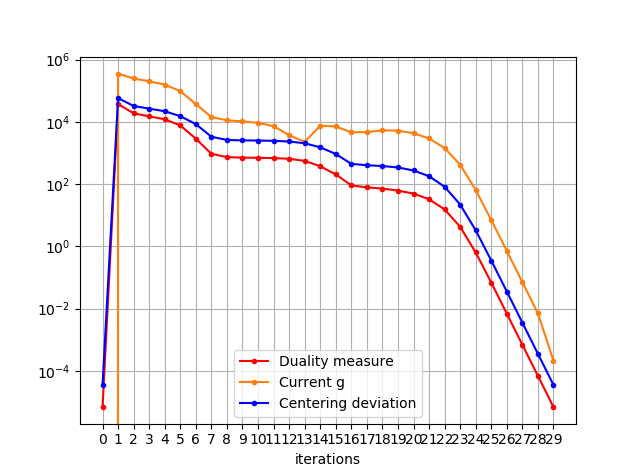
\includegraphics[width= 7 cm]{for_aff1}} \qquad%
\subfloat[Affine algorithm with MIP]{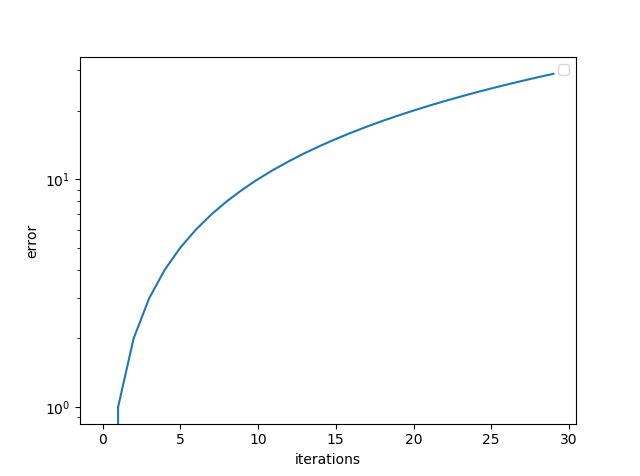
\includegraphics[width= 7 cm]{for_aff2}}\\
\subfloat[Affine algorithm with STP]{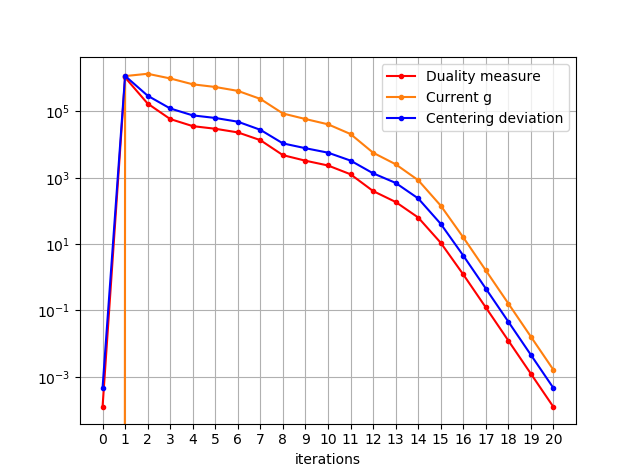
\includegraphics[width= 7 cm]{for_aff3}} \qquad%
\subfloat[Affine algorithm with STP]{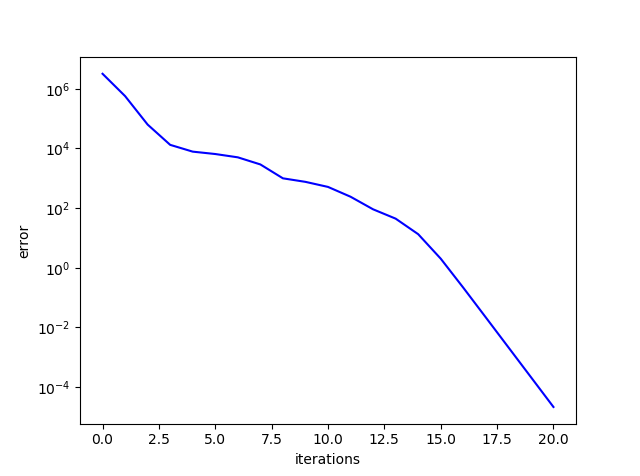
\includegraphics[width= 7 cm]{for_aff4}}\\
\subfloat[LPF 1 algorithm with MIP and with STP]{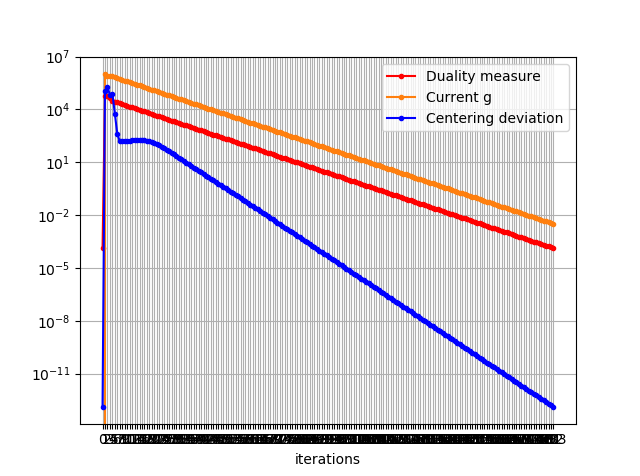
\includegraphics[width= 7 cm]{for_LPF1}} \qquad%
\subfloat[LPF 1 algorithm]{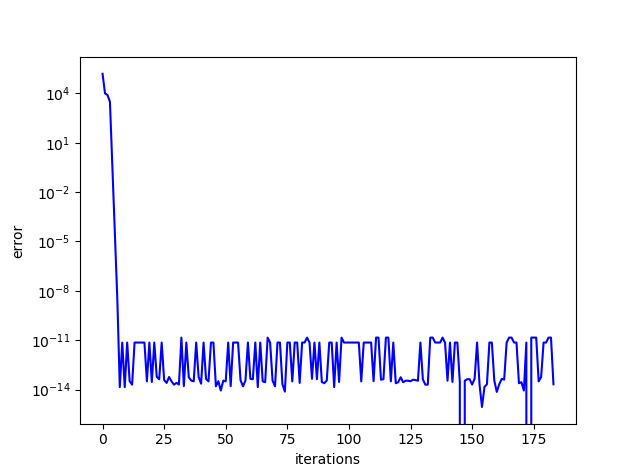
\includegraphics[width= 7 cm]{for_LPF1b}}\\
\subfloat[LPF 2 algorithm with MIP and with STP]{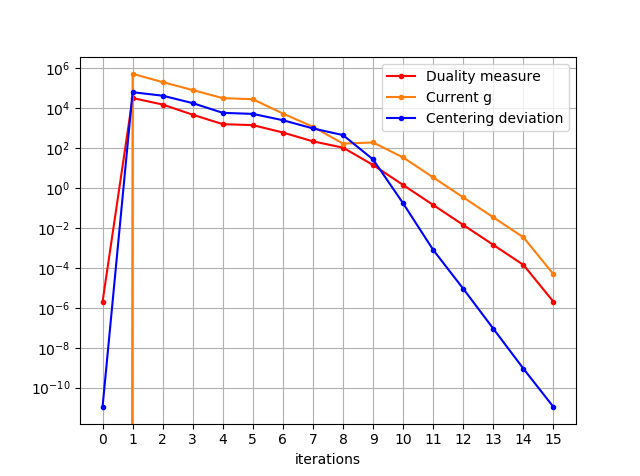
\includegraphics[width= 7 cm]{for_LPF2}} \qquad%
\subfloat[LPF 2 algorithm]{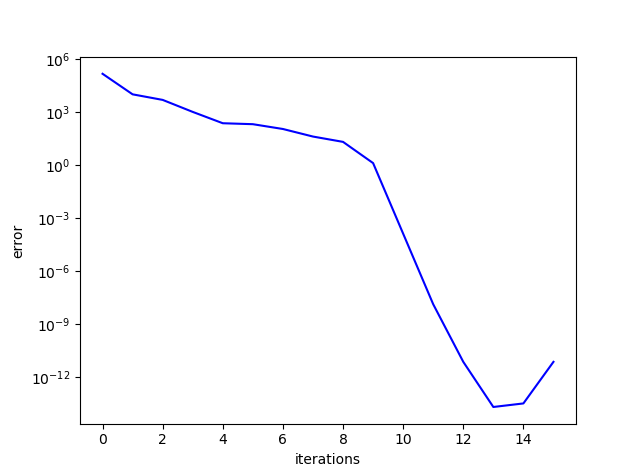
\includegraphics[width= 7 cm]{for_LPF2b}}\\
\end{figure}
\begin{figure}\caption{\label{figure:for2}Execution of the predictor-corrector IPMs to solve the forest service allocation LP model: }
\subfloat[PC LPF algorithm with MIP]{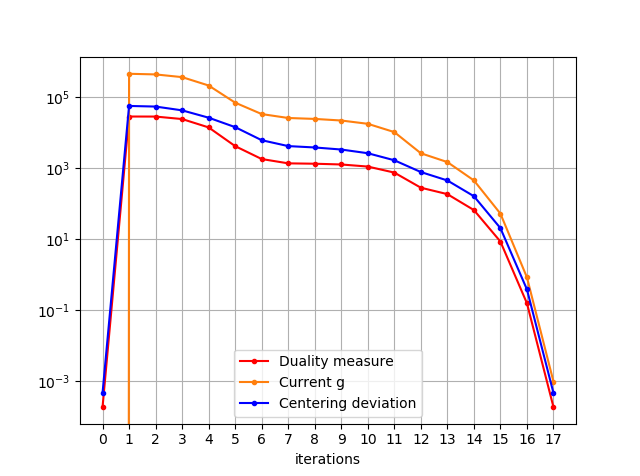
\includegraphics[width= 7 cm]{for_PCLPF}} \qquad%
\subfloat[PC LPF algorithm with MIP]{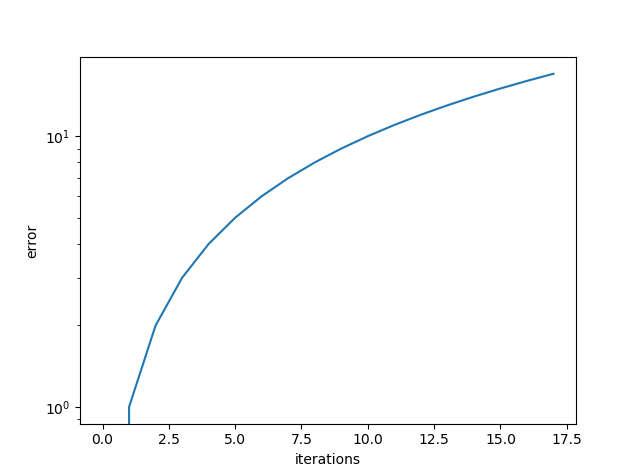
\includegraphics[width= 7 cm]{for_PCLPFb}}\\
\subfloat[PC LPF algorithm with STP 1]{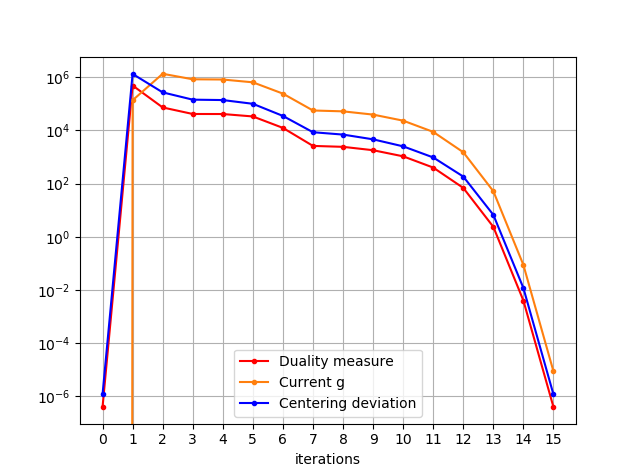
\includegraphics[width= 7 cm]{for_PCLPF2}} \qquad%
\subfloat[PC LPF algorithm with STP 1]{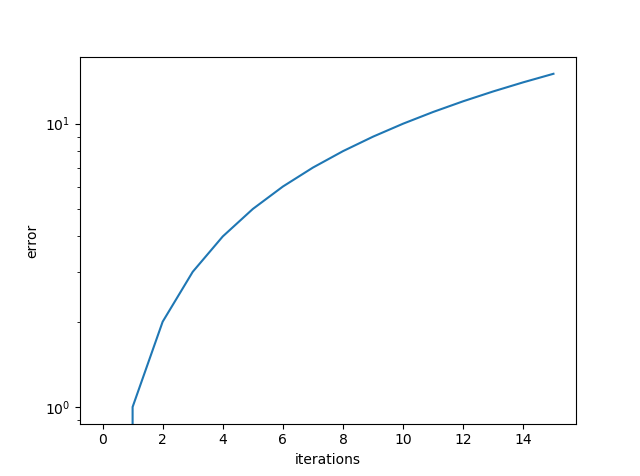
\includegraphics[width= 7 cm]{for_PCLPF2b}}\\
\subfloat[Mehrotra's algorithm]{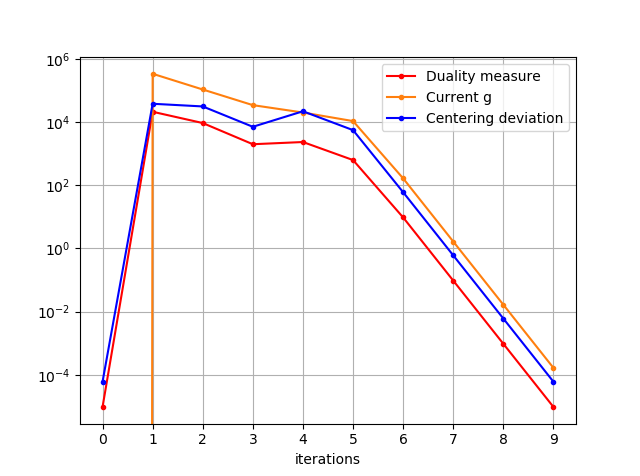
\includegraphics[width= 7 cm]{for_MER}} \qquad%
\subfloat[Mehrotra's algorithm]{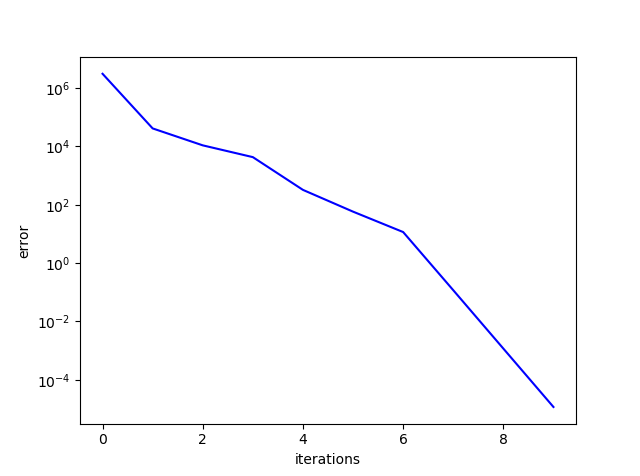
\includegraphics[width= 7 cm]{for_MERb}}\\
\end{figure}

\begin{table}[]\caption{\label{table:PNV}Numerical results obtained by the codes.}
	\begin{tabular}{cclcll}
		\hline		\textbf{} & \textbf{Initial point} & \multicolumn{1}{c}{\textbf{Optimal value}} & \textbf{Iterations number} & \multicolumn{1}{c}{\textbf{$\mu$}} & \multicolumn{1}{c}{\textbf{Residual} Res} \\ \hline
		\multicolumn{1}{c|}{\multirow{2}{*}{\textbf{Affine}}} & MIP & 3.225150E+05 & 29 & 6.928439E-06 & 2.44385E-09 \\
		\multicolumn{1}{c|}{} & STP1 & 3.225150E+05 & 20 & 2.14906E-05 & 8.50167E-09 \\ \hline
		\multicolumn{1}{c|}{\multirow{2}{*}{\textbf{LPF 1}}} & MIP & 3.22514998E+05 & 183 & 1.340977E-04 & 1.835235E-16 \\
		\multicolumn{1}{c|}{} & STP1 & 3.22514998E+05 & 183 & 1.340977E-04 & 1.835235E-16 \\ \hline
		\multicolumn{1}{c|}{\multirow{2}{*}{\textbf{LPF 2}}} & MIP & 3.225150E+05 & 15 & 2.006163E-06 & 9.476658E-17 \\
		\multicolumn{1}{c|}{} & STP1 & 3.225150E+05 & 15 & 2.006163E-06 & 9.476658E-17 \\ \hline
		\multicolumn{1}{r|}{\multirow{2}{*}{\textbf{PC LPF}}} & MIP & 3.225150E+05 & 17 & 1.857490E-08 & 7.722891E-10 \\
		\multicolumn{1}{r|}{} & STP1 & 3.225150E+05 & 15 & 1.946073E-08 & 5.089058E-15 \\ \hline
		\multicolumn{1}{c|}{\multirow{2}{*}{\textbf{Mehrotra}}} & MIP & 3.225150E+05 & 9 & 9.526700E-06 & 6.072557E-13 \\
		\multicolumn{1}{c|}{} & STP1 & 3.225150E+05 & 9 & 9.526700E-06 & 3.739456E-13 \\ \hline
	\end{tabular}
\end{table}
With Figure \ref{figure:for} and Figure \ref{figure:for2} this conjecture it is illustrated.\\ 
The affine algorithm achieves the solution in fiewer iterations with STP 1 but the velocity to reach the feasible region is similar with both strategies (see graphic (b) and (d)). Instead, the sequence computed by LPF 1 reaches the feasible region after less than 25 iterations, then the performance gets worse;  in fact, although the computational cost is high, the rate of speed of the dual gap $g$ doesn't improve.  
In the LPF 2 the improvement of $g$ is noticeable: when the primal-dual point sequence approaches to $\mathcal{F}$, $\mu$ tends to 0 with more velocity.\\ 
Now we look at the predictor-corrector methods in Figure \ref{figure:for2}: the performance of choosing $\sigma$ adaptively is evident in Mehrotra's algorithm.
In fact we see that, when the centering deviation $\delta$ grows (and the primal-dual iterate moves away from $\mathcal{C}$), the duality gap's velocity increases. Alternatively, in the LPF method the predictor-corrector strategy can't improve the duality gap since there is the restriction of the neighborhood $\mathcal{N}_{-\infty}$.\\
It is interesting looking that PC LPF and the Affine method compute primal-dual points that have a similar behaviour to the convergence to the feasible set $\mathcal{F}$, as we can see in the graphics (b) of Figure \ref{figure:for} and (b) and (d) of Figure \ref{figure:for2}.\\
We conclude that the best performancce of Mehrotra's method is clear in (f) of Figure \ref{figure:for2}: the speed of convergence is almost linear.
\newpage
\section{Swedish steel model}
As allocation models split a resource, instead blending models combine them. Various applications blend everything from chemicals, to diets, to metals, to animal food: these problems are formulated in a LP model in which you have to decide what mix of ingredients best fulfills specified output requirements. In this section the Swedish steel problem is proposed.\\
The steel industry confronts a blending problem when it melts materials in high-temperature furnaces to manufacture new alloys from scrap. Fagersta AB of Fagersta, in Sweden, is one of many companies that have used mathematical programming to plan this steel blending \cite{SSM}.\\
An optimization arises when a furnace is charged. Scrap in the available inventory is combined with a pure additives to produce a blend having the required percentages of various chemical elements. It is critical to make maximum use of scrap because addittives are much more expensive. In this research we assess that the Swedish steel making will produce a 1000-kilogram furnace charge and all steel consists primarly of iron. Table \ref{table:carbon} with fictitious data shows the much smaller fractions of carbon, nickel, chromium, and molybdenum in the four available supplies of scrap. It also shows the three higher-cost additives that can be used and the acceptable ranges for the resulting blend.\\
\begin{table}[h]\caption{\label{table:carbon}Data for Swedish Steel LP model.}
\begin{center}
	\begin{tabular}{@{}lllllll@{}}
		\toprule
		& Carbon & Nickel & Chromium & Molybdenum & Available & Cost \\ \midrule
		First scrap   & 0.80   & 18     & 12       & -          & 75        & 16   \\
		Second scrap  & 0.70   & -      & -        & -          & 250       & 10   \\
		Third scrap   & 0.85   & -      & -        & -          & Unlimited & 8    \\
		Fourth scrap  & 0.40   & -      & -        & -          & Unlimited & 9    \\
		Nickel        & -      & 100    & -        & -          & Unlimited & 48   \\
		Chronium      & -      & -      & 100      & 100        & Unlimited & 60   \\
		Molybdenum    & -      & -      & -        & -          & Unlimited & 53   \\ \midrule
		Minimum blend & 0.65   & 3.0    & 1.0      & 1.1        &           &      \\ 
		Maximum blend & 0.75   & 3.5    & 1.2      & 1.3        &           &      \\ \midrule
	\end{tabular}
\end{center}
\end{table}
The principal decision variables in blending models specify how much of each available ingredient to include in the mix. In the Swedish Steel example we define the decision variables $x_{j}$, where $j = 1, \dots, 4$ refers to the four supplies of scrap and $j = 5, \dots, 7$ refers to the pure additives.\\
We have also upper and lower limits on the fraction of carbon, nickel, chromium and molybdenum in the mix; each constraint will have the form: 
\begin{equation*}
\sum\limits_{j}\Bigg(\begin{tabular}{l}
 fraction in\\
jth\\
ingredient\\
\end{tabular}
\Bigg)\Bigg(\begin{tabular}{l}
 amount of\\
jth\\
ingredient\\
\end{tabular}\Bigg)
\begin{tabular}{l}
     \geq\\
	\text{or}\\
	\leq\\
\end{tabular}
	\Bigg(\begin{tabular}{l}
		allowed\\
		fraction in\\
		the blend\\
	\end{tabular}
	\Bigg)
\Bigg(\begin{tabular}{l}
		blend\\
		total\\
		weught\\
	\end{tabular}
	\Bigg).
\end{equation*}		
The compostion constraints have been simplified by taking the blend total weight fixed at 1000 kilograms, in parenthesis in the formulation below. Collecting all the elements, the LP model of the Swedish example is: 
\begin{align*}
\min16x_{1}+10x_{2}+8x_{3}+9x_{4}+48x_{5}+60x_{6}+53x_{7}& &\text{(cost)}&\\
x_{1}+x_{2}+x_{3}+x_{4}+x_{5}+x_{6} + x_{7}&= 1000&\text{(weight)}&\\
0.008x_{1}+0.007x_{2}+0.0085x_{3}+0.004x_{4}&\geq 0.0065(1000)&\text{(carbon)}&\\
0.008x_{1}+0.007x_{2} + 0.0085x_{3} + 0.004x_{4}&\leq 0.0075(1000)&\\
0.180x_{1}+0.032x_{2} + 1.0x_{5}&\geq 0.030(1000)& \text{(nickel)}&\\
0.180x_{1}+0.032x_{2} + 1.0x_{5}&\leq 0.035(1000)&\\
0.120x_{1}+0.011x_{2} + 1.0x_{6}&\geq 0.010(1000)& \text{(chromium)}&\\
0.120x_{1}+0.011x_{2} + 1.0x_{6}&\leq 0.012(1000)&\\
0.001x_{2} + 1.0x_{7}&\geq 0.011(1000)& \text{(molybdenum)}&\\
0.001x_{2} + 1.0x_{7}&\leq 0.013(1000)&\\
x_{1}&\leq 75&\text{(available)}&\\
x_{2}&\leq 250 &&\\
x_{1},\dots, x_{7}\geq 0.\\
\end{align*}
According to \cite{RR} and confirmed by the results of the codes, the total cost of an optimal charge is 9953.72 kr, with the following optimal solution of the canonical LP problem:
\begin{align*}
x_{1}^{*} &=  75\text{ kg,} & x_{2}^{*}&=  90.91\text{ kg,} & x_{3}^{*} &= 672.28 \text{ kg,} & x_{4}^{*} &= 137.31 \text{ kg,}\\
x_{5}^{*} &= 13.59 \text{ kg,}& x_{6}^{*}&= 0\text{ kg,}  & x_{7}^{*} &= 10.91 \text{ kg.} &&\\
\end{align*}
\begin{table}[t]\caption{\label{table:SWE}Numerical results obtained by the codes.}
	\begin{tabular}{cclcll}
		\hline		\textbf{} & \textbf{Initial point} & \multicolumn{1}{c}{\textbf{Optimal value}} & \textbf{Iterations number} & \multicolumn{1}{c}{\textbf{$\mu$}} & \multicolumn{1}{c}{\textbf{Residual} Res} \\ \hline
		\multicolumn{1}{c|}{\multirow{2}{*}{\textbf{Affine}}} & MIP & 9.95367172E+03 & 17 & 1.086069E-06 & 4.688545E-11 \\
		\multicolumn{1}{c|}{} & STP1 & 9.95367174E+03 & 22 & 4.511383E-06 & 3.399852E-10 \\ \hline
		\multicolumn{1}{c|}{\multirow{2}{*}{\textbf{LPF 1}}} & MIP & 9.95367175E+03 & 161 & 5.835742E-06 & 2.193332E-16 \\
		\multicolumn{1}{c|}{} & STP1 & 9.95367173E+03 & 161 & 5.835742E-06 & 2.193332E-16 \\ \hline
		\multicolumn{1}{c|}{\multirow{2}{*}{\textbf{LPF 2}}} & MIP & 9.95367173E+03 & 13 & 2.265246E-06 & 1.120302E-16 \\
		\multicolumn{1}{c|}{} & STP1 & 9.95367172E+03 & 13 & 2.265246E-06 & 1.120302E-16 \\ \hline
		\multicolumn{1}{r|}{\multirow{2}{*}{\textbf{PC LPF}}} & MIP & 9.95367172E+03 & 14 & 1.037639E-08 & 8.081460E-14 \\
		\multicolumn{1}{r|}{} & STP1 & 9.95367172E+03 & 15 & 1.797854E-09 & 7.265413E-15 \\ \hline
		\multicolumn{1}{c|}{\multirow{2}{*}{\textbf{Mehrotra}}} & MIP & 9.95367172E+03 & 8 & 8.932283E-07 & 6.682737E-12 \\
		\multicolumn{1}{c|}{} & STP1 & 9.95367172E+03 & 10 & 1.822205E-07 & 8.825683E-15 \\ \hline
	\end{tabular}
\end{table}
Now it is developed an analysis that leads to 
some different results respect to the previous one. First of all, we observe in Table \ref{table:SWE} that the starting point strategy is indifferent, except for the Affine and the both predictor-corrector algorithms.\\As already occured, the LPF 1 requires a huge computational cost respect to the others and, after achieved the boundary of the feasible set, the duality measure $\mu$ is far to satisfy the termination conditions. In this case the number of iterations computing LPF 2 is the smallest comparing to the other LPF's ones, but the $\mu$ reveals that it is not the most accurate in term of convergence.\\
In Figure \ref{figure:swe} the graphics (e) and (f) confirm the bad behaviour of LPF1 and (h) disproves the asymptotic convergence in LPF 2: in the last iterates it computes points that move away from the feasible set.\\
In Figure \ref{figure:swe2}, it is clear that the two predictor-corrector IPMs perform better with STP. In fact there is an anomaly in the graphic (c), where the dual gap doesn't decrease with regularity, even if the sketch of the feasiblity error speed (d) shows a linear progression. \\
Now we investigate the Mehrotra's method: since the centering deviation $\sigma$ doesn't increase and hence it is not necessary an adaptive $\sigma$ to obtain aggressive reduction of $\mu$, as we see in (e) and in (g), it seems superior.\\
It is not gathered the effectiveness of the heuristic choice of $\sigma$ in a geometric point of view in the Mehrotra's iterates: they stay particularly close to the central path $\mathcal{C}$ while steadily going to the optimal solution. 
Although this, we can state the important rule of the adaptive centering parameter in long-path following method: even if PC LPF requires more iterations, it does not generate a irregular convergence. \\The optimal cost value solutions in Table \ref{table:SWE} reassert the power of the predictor-corrector algorithms.   
\begin{figure}\caption{\label{figure:swe}Execution of the IPMs to solve Swedish steel LP model:}
	\subfloat[Affine algorithm with MIP]{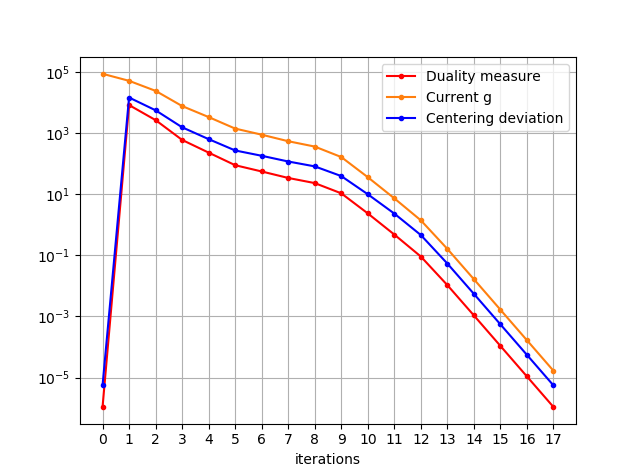
\includegraphics[width= 7 cm]{swe_aff1}} \qquad%
	\subfloat[Affine algorithm with MIP]{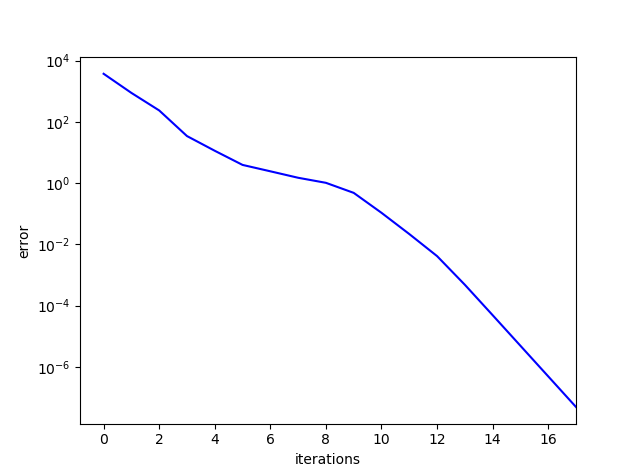
\includegraphics[width= 7 cm]{swe_aff2}}\\
	\subfloat[Affine algorithm with STP]{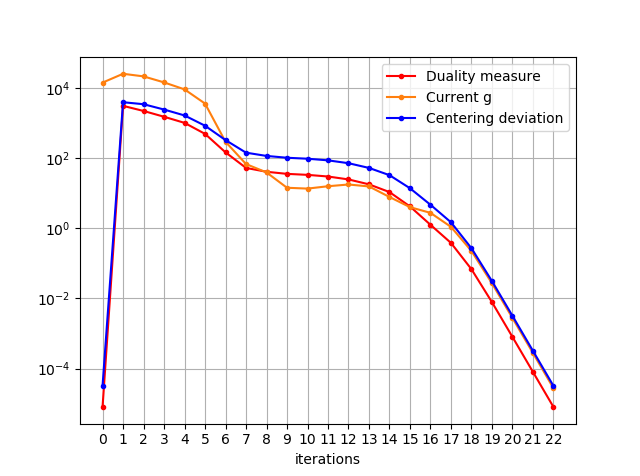
\includegraphics[width= 7 cm]{swe_aff3}} \qquad%
	\subfloat[Affine algorithm with STP]{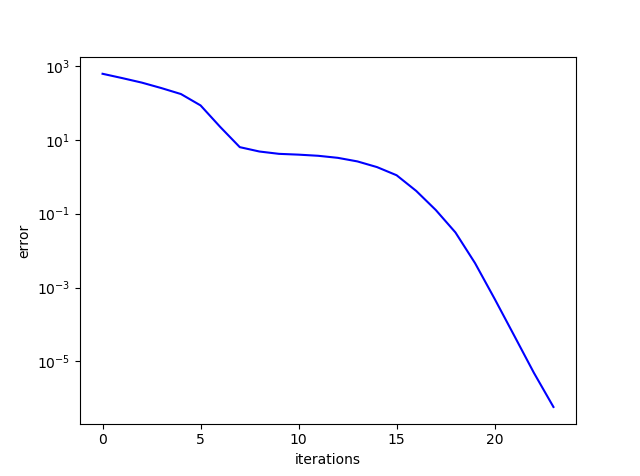
\includegraphics[width= 7 cm]{swe_aff4}}\\
	\subfloat[LPF 1 algorithm with MIP and STP]{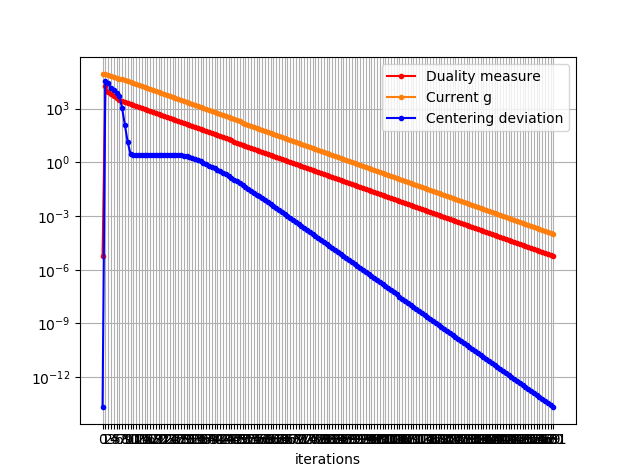
\includegraphics[width= 7 cm]{swe_LPF1}} \qquad%
	\subfloat[LPF 1 algorithm with MIP and STP]{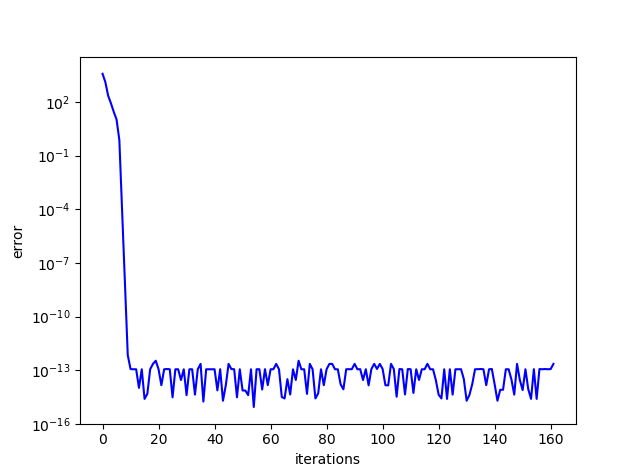
\includegraphics[width= 7 cm]{swe_LPF1b}}\\
	\subfloat[LPF 2 algorithm with MIP and STP]{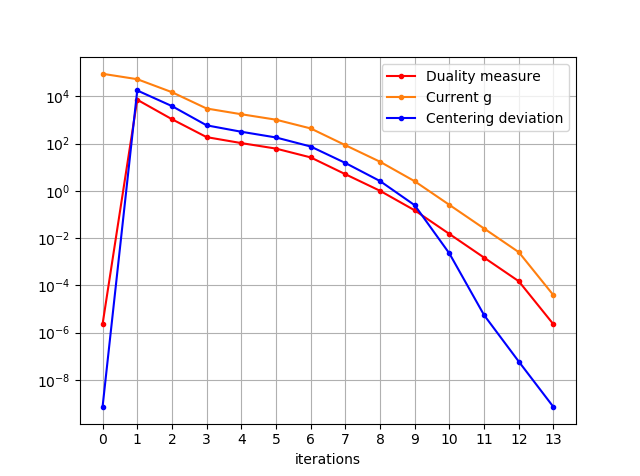
\includegraphics[width= 7 cm]{swe_LPF2}} \qquad%
	\subfloat[LPF 2 algorithm with MIP and STP]{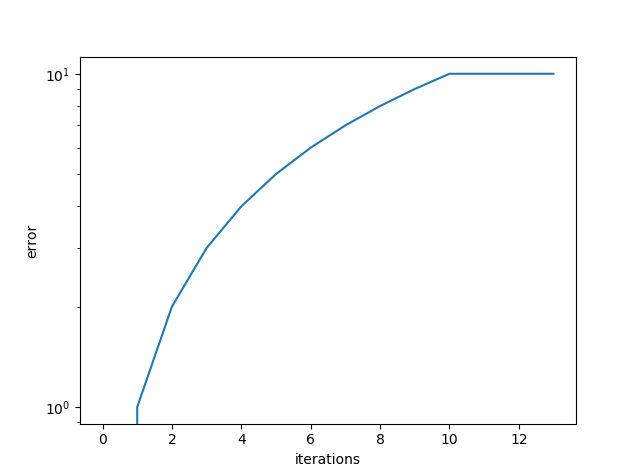
\includegraphics[width= 7 cm]{swe_LPF2b}}\\
\end{figure}
\begin{figure}\caption{\label{figure:swe2}Execution of predictor-corrector IPMs to solve Swedish steel LP model:}
	\subfloat[PC LPF algorithm with MIP]{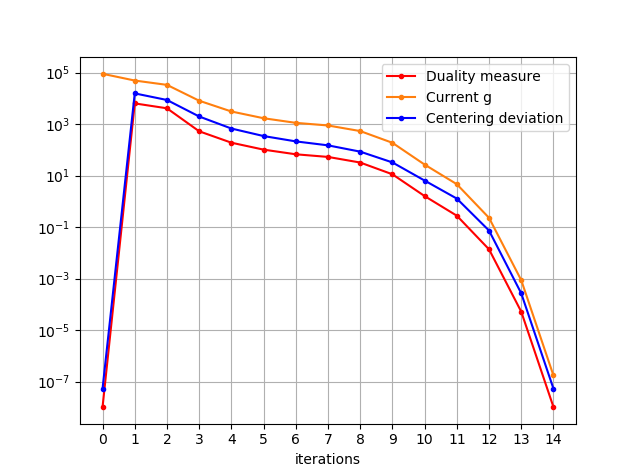
\includegraphics[width= 7 cm]{swe_PCLPF}} \qquad%
	\subfloat[PC LPF algorithm with MIP]{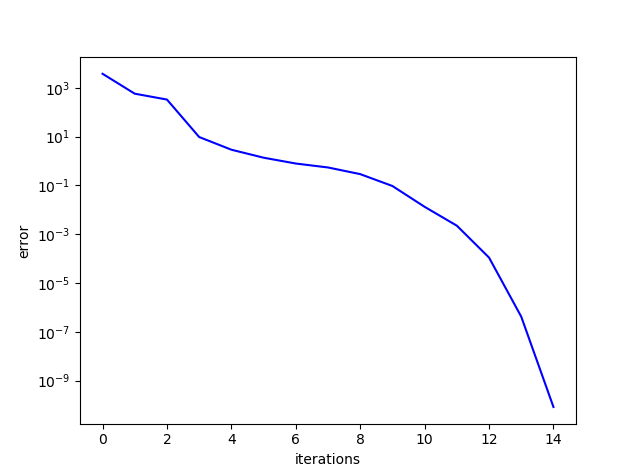
\includegraphics[width= 7 cm]{swe_PCLPFb}}\\
	\subfloat[PC LPF algorithm with STP]{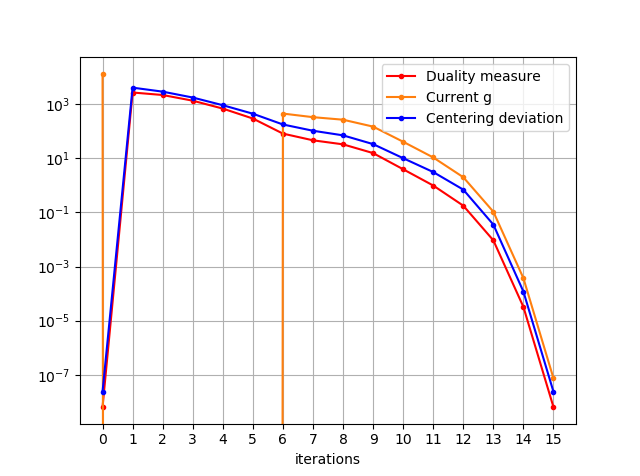
\includegraphics[width= 7 cm]{swe_PCLPF2}} \qquad%
	\subfloat[PC LPF algorithm with STP]{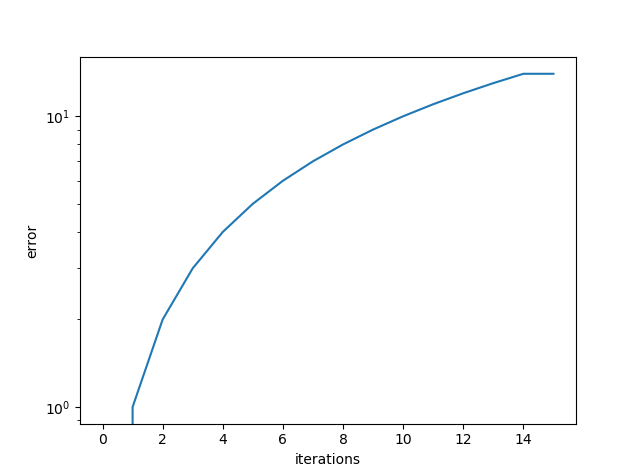
\includegraphics[width= 7 cm]{swe_PCLPF2b}}\\
	\subfloat[Mehrotra's algorithm with MIP]{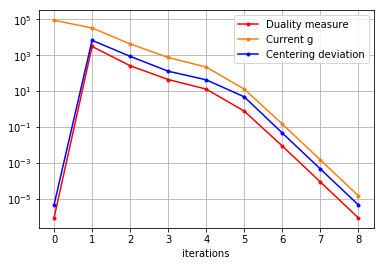
\includegraphics[width= 7 cm]{swe_MER}} \qquad%
	\subfloat[Mehrotra's algorithm with MIP]{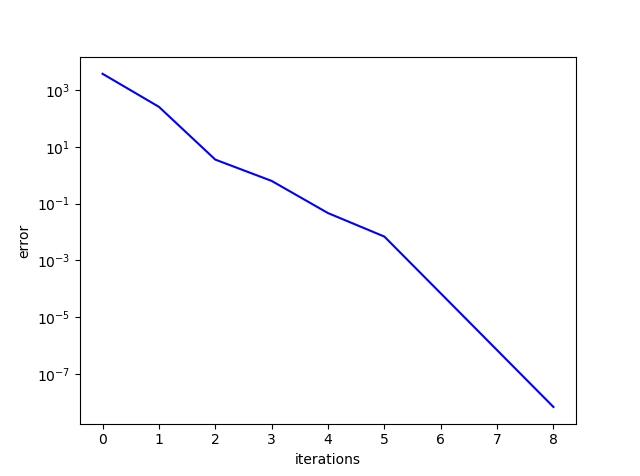
\includegraphics[width= 7 cm]{swe_MERb}}\\	\subfloat[Mehrotra's algorithm with STP]{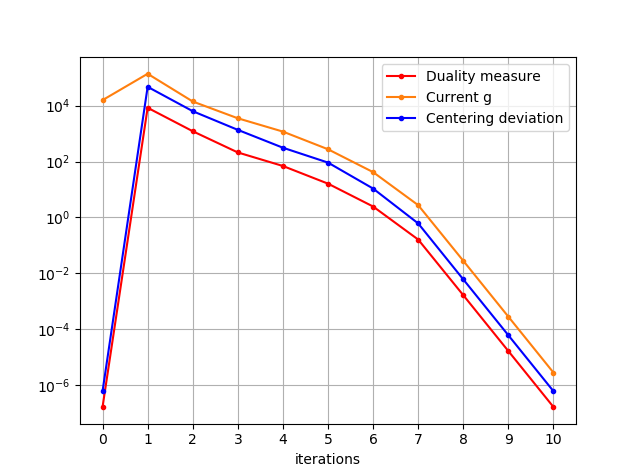
\includegraphics[width= 7 cm]{swe_MER2}} \qquad%
	\subfloat[Mehrotra's algorithm with STP]{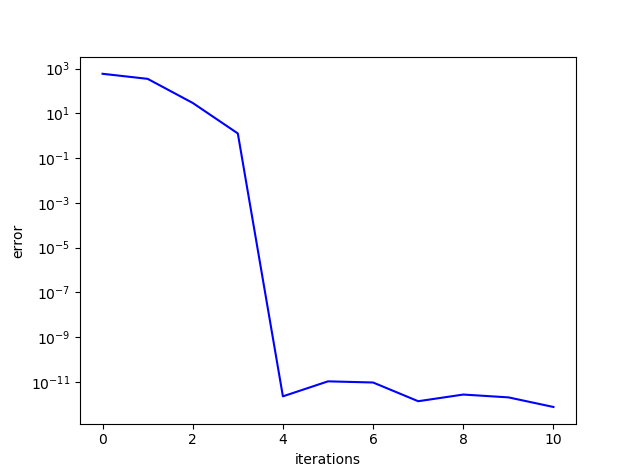
\includegraphics[width= 7 cm]{swe_MER2b}}\\
\end{figure}
\newpage
\section{Tubular products operations planning}
Another classic LP form deals with operation planning. In organizations ranging from volunteer, to government, to manifacturing, to distribution, planners must decide what to do and when and where to do it.\\
The Tubular Products Division (TP) of Babcock and Wilcox encountered a problem in investigating how work should be reallocated upon opening a new mill \cite{FEM}. TP manifactured steels tubing in a variety of sizes and for many different uses, including electrical power generation. At the time of the study three mills handled production. The object was to consider how a fourth mill of different configuration would affect the optimal distribution of work (and associated cost) among the mills.\\Table \ref{tab:TPdata} shows fictional data for existing mills 1 to 3 and one design for new mill 4, versus an array of 16 products. The products comprise all combinations of standard or high-pressure tubing: $\frac{1}{2}-$, $1-$, $2-$ or $8-$inch diameters, and thick or thin tube walls. It is included the cost (in dollars) per 1000 pounds of each product according to which mill does the work, and the required processing time (in hours) per 1000 pounds produced. Missing values indicate products that cannot be manufactured feasibly at the mill indicated.\\
It is also assumed division-wide demand for each of the 16 products in thousands of pounds per week. At present the three existing mills 1 to 3 have 800, 480 and 1280 hours per week of effective production capacity, respectively. New mill 4 is planned for 960 hours per week (see Table \ref{tab:TPdata}).\\
Here the problem has two index dimensions: $i= 1, \dots, 16$ rappresents the product number and $j=1, \dots, 4$ the mill number. Instead, the decision variables and the constants are:
\begin{itemize}
	\item $x_{i,j}$ is the amount of product $i$ producted at mill $m$ (in thousands of pounds per week),
	\item $c_{i,j}$ is the unit cost of producing product $i$ at mill $j$,
	\item $t_{i,j}$ is the unit time to manufacture product $i$ at mill $j$,
	\item $d_{i}$ is the weekly demand for product $i$,
	\item $b_{j}$ is the given production capacity at mill $j$.
\end{itemize}
The model required is:
\begin{align*}
\min&\sum_{i=1}^{16}\sum_{j=1}^{4} c_{i,j}x_{i,j}&(\text{total cost})\\
\text{s.t}\;\; & \sum_{j=1}^{4}x_{i,j}\geq d_{i},\;\;\;\;\;\;\;\;\text{for }i = 1, \dots,16&(\text{demands})\\
&\sum_{i=1}^{16}t_{i,j}x_{i,j}\leq b_{j},\;\;\;\;\text{for }j = 1, \dots,4&(\text{capacities})\\
&x_{i,j}\geq 0, \;\;\;\;\;\;\;\;\;\;\;\;\;\;\;\;\text{for }i = 1,\dots,16,\;\;\;\;j = 1,\dots,4.
\end{align*}
One system of main constraints enforces product demands and other the mill capacities.
The objective function minimizes total production cost and the total optimal weekly cost is \$ 252607,14, valued at the optimal solution $x^{*}$ with all entries $x_{i,j} = 0$, except for:
\begin{table}[h]
	\begin{tabular}{llllll}
		\textbf{Mill 1:} & $x_{4,1}=100$, & $x_{7,1}=630$, & $x_{12,1}=500$, & $x_{15,1}=254,286$, & $x_{16,1}=725,714$; \\
		\textbf{Mill 2:} & $x_{2,2}=685,714$, & $x_{4,2}=34,285$, & $x_{8,2}=240$, & $x_{9,2}=75$, & $x_{13,2}=22$; \\
		\textbf{Mill 3:} & $x_{3,3}=50$, & $x_{7,3}=22$, & $x_{11,3}=353$, & $x_{15,3}=55$; &  \\
		\textbf{Mill 4:} & $x_{2,4}=55$, & $x_{6,4}=125$, & $x_{10,4}=35$, & $x_{12,4}=100$, & $x_{16,4}=10$.
	\end{tabular}
\end{table}

\begin{center}
\begin{table}[h]
	\begin{tabular}{ccccccccccc}
		\hline
		& \textbf{} & \multicolumn{2}{c}{\textbf{Mill 1}} & \multicolumn{2}{c}{\textbf{Mill 2}} & \multicolumn{2}{c}{\textbf{Mill 3}} & \multicolumn{2}{c}{\textbf{Mill 4}} & \textbf{} \\
		&  & Cost, & Hours, & Cost, & Hours, & Cost, & Hours, & Cost, & Hours, & Weekly dem \\ \cline{3-10}
		& \textbf{Product} & \textbf{$c_{i,1}$} & \textbf{$t_{i,1}$} & \textbf{$c_{i,1}$} & \textbf{$t_{i,2}$} & \textbf{$c_{i,2}$} & \textbf{$t_{i,3}$} & \textbf{$c_{i,3}$} & \textbf{$t_{i,4}$} & \textbf{$d_{i}$} \\ \hline
		\textbf{Std} &  &  &  &  &  &  &  &  &  &  \\ \cline{1-1}
		1 & $\frac{1}{2}$in.thick & 90 & 0.8 & 75 & 0.7 & 70 & 0.5 & 63 & 0.6 & 100 \\
		2 & $\frac{1}{2}$in.thin & 80 & 0.8 & 70 & 0.7 & 65 & 0.5 & 60 & 0.6 & 630 \\
		3 & 1in.thick & 104 & 0.8 & 85 & 0.7 & 83 & 0.5 & 77 & 0.6 & 500 \\
		4 & 1in.thin & 98 & 0.8 & 79 & 0.7 & 80 & 0.5 & 74 & 0.6 & 980 \\
		5 & 2in.thick & 123 & 0.8 & 101 & 0.7 & 110 & 0.5 & 99 & 0.6 & 720 \\
		6 & 2in.thin & 113 & 0.8 & 94 & 0.7 & 100 & 0.5 & 84 & 0.6 & 240 \\
		7 & 8in.thick & - & - & 160 & 0.9 & 156 & 0.5 & 140 & 0.6 & 75 \\
		8 & 8in.thin & - & - & 142 & 0.9 & 150 & 0.5 & 130 & 0.6 & 22 \\ \hline
		\textbf{Press.} &  &  &  &  &  &  &  &  &  &  \\ \cline{1-1}
		9 & $\frac{1}{2}$in.thick & 140 & 1.5 & 110 & 0.9 & - & - & 122 & 1.2 & 50 \\
		10 & $\frac{1}{2}$in.thin & 124 & 1.5 & 96 & 0.9 & - & - & 101 & 1.2 & 22 \\
		11 & 1in.thick & 160 & 1.5 & 133 & 0.9 & - & - & 138 & 1.2 & 353 \\
		12 & 1in.thin & 124 & 1.5 & 127 & 0.9 & - & - & 133 & 1.2 & 55 \\
		13 & 2in.thick & 202 & 1.5 & 150 & 0.9 & - & - & 160 & 1.2 & 125 \\
		14 & 2in.thin & 190 & 1.5 & 141 & 0.9 & - & - & 140 & 1.2 & 35 \\
		15 & 8in.thick & - & - & 190 & 1.0 & - & - & 220 & 1.5 & 100 \\
		16 & 8in.thin & - & - & 175 & 1.0 & - & - & 200 & 1.5 & 10 \\ \hline
	\end{tabular}\caption{\label{tab:TPdata}Tubular products model data.}
\end{table}
\end{center}

\\In Table \ref{table:TP} we can notice that LPF 1 algorithm doesn't work. Instead, LPF 2 finds the exact solution with the same number of iterations with both two initial point strategies. \\
Focusing on the PC methods, again their computational cost is smaller, above all the Mehrotra's method, as expected, and they achieve a smaller duality measure $\mu$ in the $\epsilon$ optiml solution.\\ It is interesting to note the different number of iterations computed by the PC algorithms with the MIP and with STP strategies. For the PC LPF method, the speed of convergence of $\{\mu_{k}\}$ and of the sequence points $\{(x_{k},\lambda_{k},s_{k})\}$ to the feasible set $\mathcal{F}$ is linear, in comparing to the irreguliaty of LPF 2 computation progress, illustrated in (e) and in (f) of Figure \ref{figure:tub}.
The predictor-corrector maneuver in (g) of Figure \ref{figure:tub2} is clear: when the centering deviation increases, then the speed of the the duality measure increases, maintaining such a linearity (see the fourth iteration).\\
Also in this case, we can assert that the adaptivity choice of the centering parameter $\sigma$ in LPF is not functional as in Mehrotra's algorithm: in a geometric point of view we see the restiction of the neighboorhood does not allow a movement of the sequence to step away from $\mathcal{C}$ and hence improve the $\mu$ convergence speed.\\
In the end it is interesting observe the superlinear convergence of the Mehrotra's iterates to $\mathcal{F}$: it occurs in this instance a huge improvement of the points to achieve the feasibility region.
\begin{table}[]\caption{\label{table:TP}Numerical results obtained by the codes.}
	\begin{tabular}{cclcll}
		\hline		\textbf{} & \textbf{Initial point} & \multicolumn{1}{c}{\textbf{Optimal value}} & \textbf{Iterations number} & \multicolumn{1}{c}{\textbf{$\mu$}} & \multicolumn{1}{c}{\textbf{Residual} Res} \\ \hline
		\multicolumn{1}{c|}{\multirow{2}{*}{\textbf{Affine}}} & MIP & 2.52607142E+05 & 23 & 1.345159E-05 & 3.606275E-11 \\
		\multicolumn{1}{c|}{} & STP1 & 2.52607142E+05 & 26 & 2.769742E-05 & 1.823342E-09 \\ \hline
		\multicolumn{1}{c|}{\multirow{2}{*}{\textbf{LPF 1}}} & MIP & - & - & - & - \\
		\multicolumn{1}{c|}{} & STP1 & - & - & - & - \\ \hline
		\multicolumn{1}{c|}{\multirow{2}{*}{\textbf{LPF 2}}} & MIP & 2.52607143E+05 & 21 & 1.316057E-05 & 5.087151E-14 \\
		\multicolumn{1}{c|}{} & STP1 & 2.52607143E+05 & 21 & 1.316057E-05 & 5.087151E-14 \\ \hline
		\multicolumn{1}{r|}{\multirow{2}{*}{\textbf{PC-LPF}}} & MIP & 2.52607143E+05 & 20 & 8.639578E-06 & 8.284204E-13 \\
		\multicolumn{1}{r|}{} & STP1 & 2.52607143E+05 & 16 & 1.675101E-07 & 4.966188E-10 \\ \hline
		\multicolumn{1}{c|}{\multirow{2}{*}{\textbf{Mehrotra}}} & MIP & 2.52607143E+05 & 10 & 7.137129E-06 & 1.865384E-13 \\
		\multicolumn{1}{c|}{} & STP1 & 2.52607143E+05 & 11 & 7.171488E-06 & 1.459857E-12 \\ \hline
	\end{tabular}
\end{table}
\begin{figure}\caption{\label{figure:tub}Execution of the IPMs tubular production LP model:}
	\subfloat[Affine algorithm with MIP]{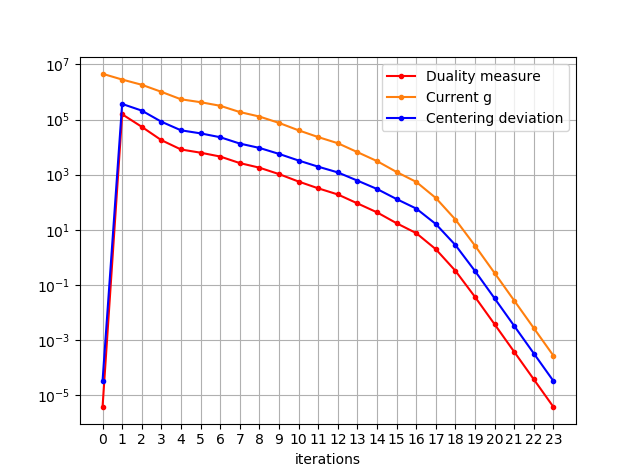
\includegraphics[width= 7 cm]{tub_aff1}} \qquad%
	\subfloat[Affine algorithm with MIP]{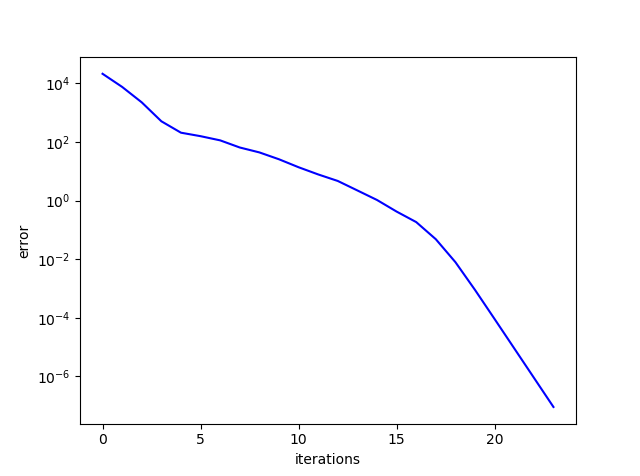
\includegraphics[width= 7 cm]{tub_aff2}}\\
	\subfloat[Affine algorithm with STP]{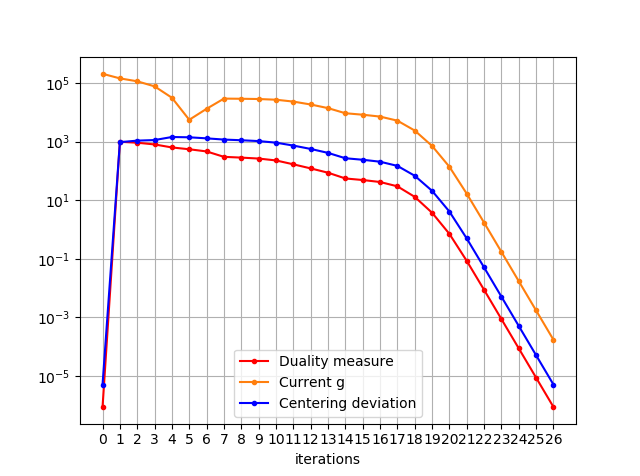
\includegraphics[width= 7 cm]{tub_aff3}} \qquad%
	\subfloat[Affine algorithm with STP]{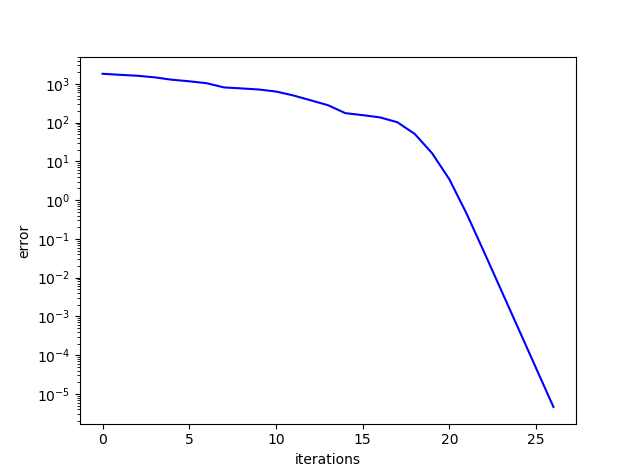
\includegraphics[width= 7 cm]{tub_aff4}}\\
	\subfloat[LPF 2 algorithm ]{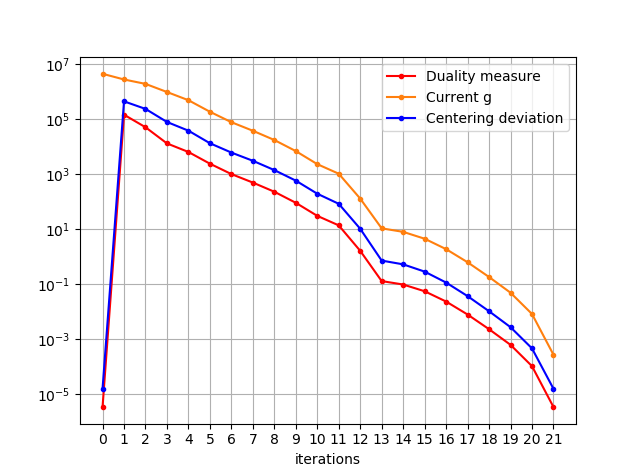
\includegraphics[width= 7 cm]{tub_LPF2}} \qquad%
	\subfloat[LPF 2 algorithm]{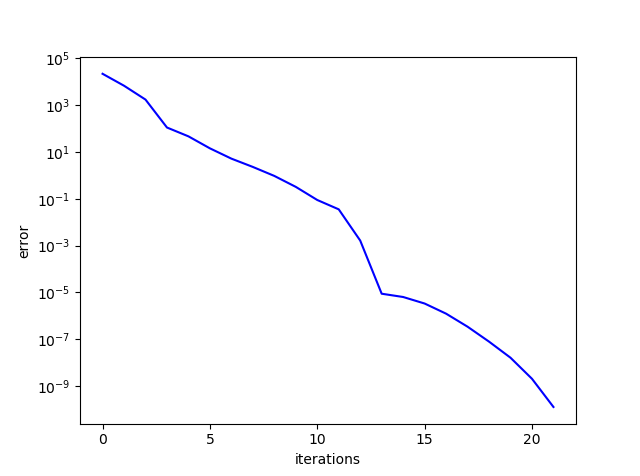
\includegraphics[width= 7 cm]{tub_LPF2b}}\\
\end{figure}
\begin{figure}\caption{\label{figure:tub2}Execution of predictor-corrector IPMs tubular production LP model:}
	\subfloat[PC LPF algorithm with MIP]{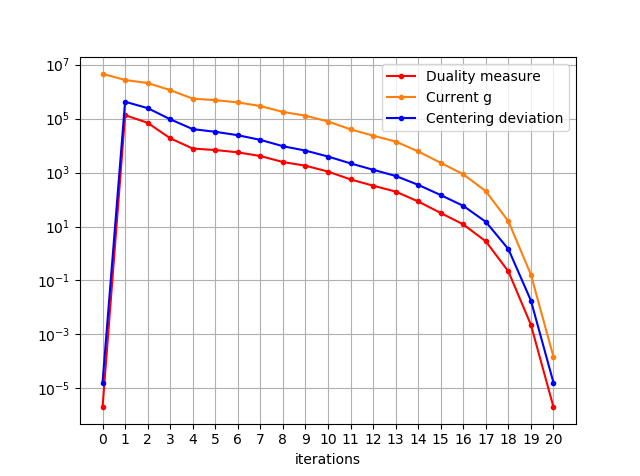
\includegraphics[width= 7 cm]{tub_PCLPF}} \qquad%
	\subfloat[PC LPF algorithm with MIP]{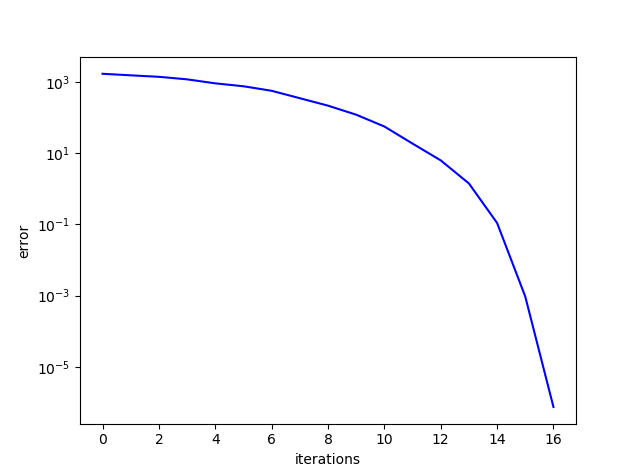
\includegraphics[width= 7 cm]{tub_PCLPFb}}\\
	\subfloat[PC LPF algorithm with STP1]{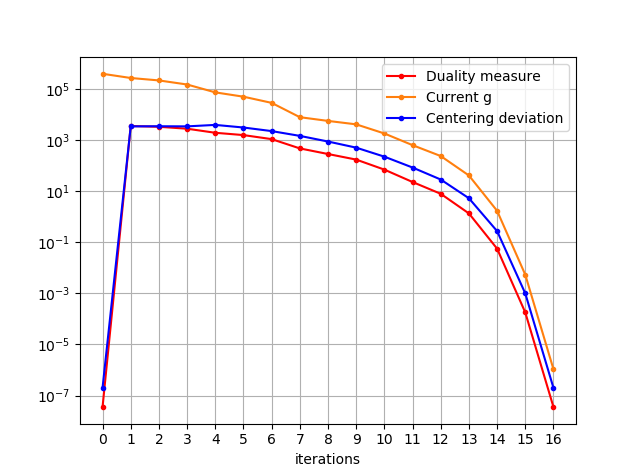
\includegraphics[width= 7 cm]{tub_PCLPF2}} \qquad%
	\subfloat[PC LPF algorithm with STP1]{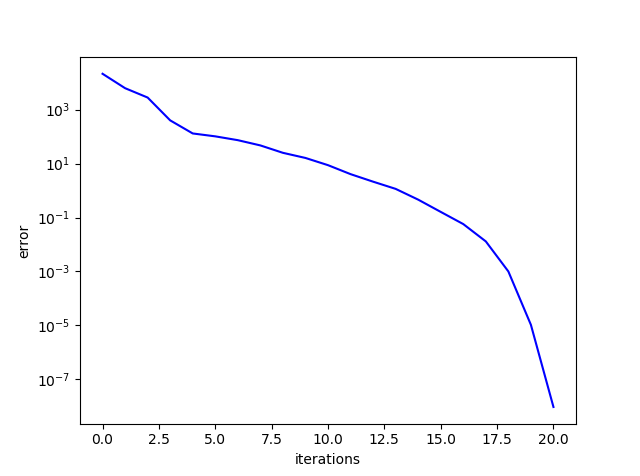
\includegraphics[width= 7 cm]{tub_PCLPF2b}}\\
	\subfloat[Mehrotra's algorithm with MIP]{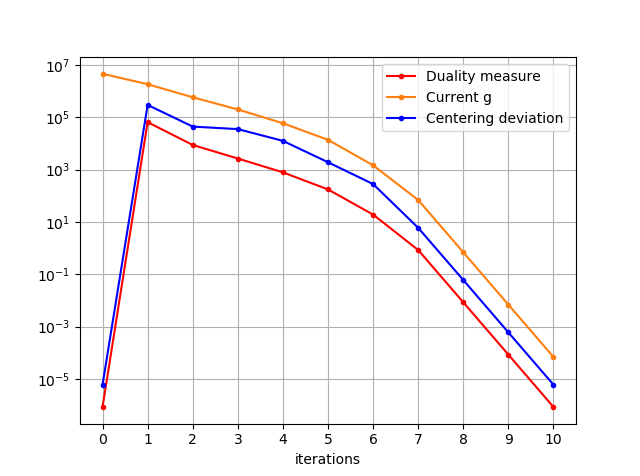
\includegraphics[width= 7 cm]{tub_MER}} \qquad%
	\subfloat[Mehrotra's algorithm with MIP]{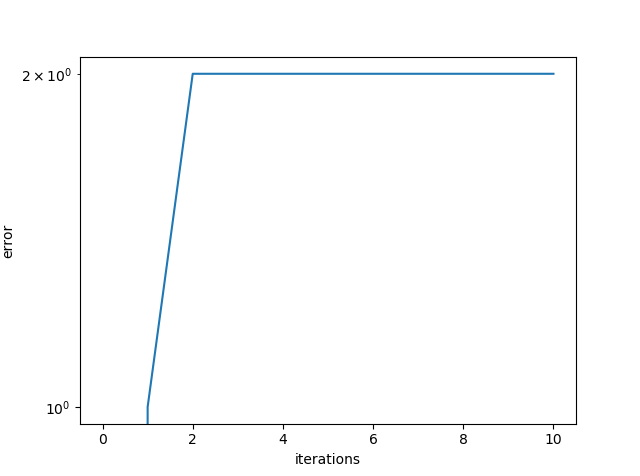
\includegraphics[width= 7 cm]{tub_MERb}}\\	\subfloat[Mehrotra's algorithm with STP1]{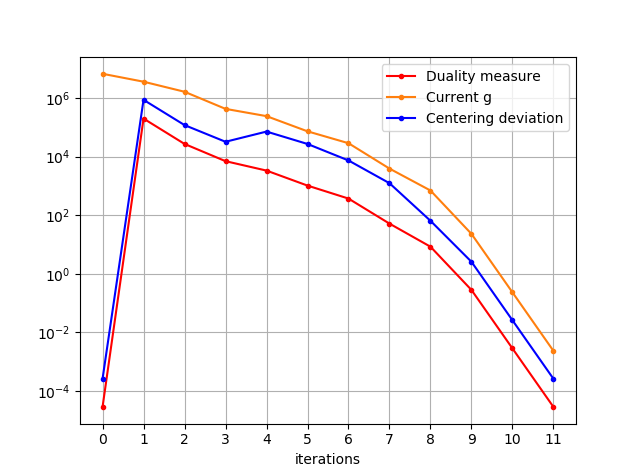
\includegraphics[width= 7 cm]{tub_MER2}} \qquad%
	\subfloat[Mehrotra's algorithm with STP1]{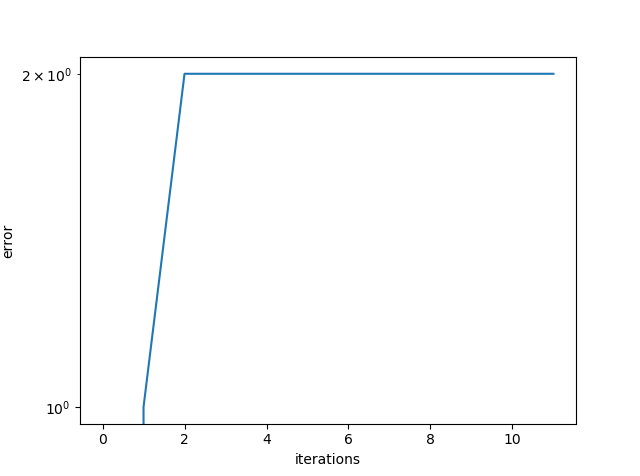
\includegraphics[width= 7 cm]{tub_MER2b}}\\
\end{figure}
\newpage
\section{Ohio National Bank shift scheduling}
Operations planning models decide what work to undertake so that available resources are used efficiently and in shift scheduling or staff planning models the work is already fixed but it is necessary to plan the resources to accomplish it.\\
The Ohio National Bank (ONB) confronted such a problem in staffing its check processing center \cite{ONB}. Checks received by the bank already have account numbers and other identifying information encoded on them. Machine operators in the check processing center key the dollar  amount of the check, which is then imprinted with the other information for computerized processing.\\Checks arrive through the business day in volumes peaking in the early evening. The fictious version will assume the arrivals printed in Table \ref{table:shiftscheduling}, in thousand. \\
\begin{table}[h]\caption{\label{table:shiftscheduling}Possible ONB arrivals schedule}
	\begin{center}
	\begin{tabular}{ll|ll}
		\hline
		\textbf{Hour} & \textbf{Arrivals} & \textbf{Hour} & \textbf{Arrivals} \\ \hline
		11:00 & 10 & 17:00 & 32 \\
		12:00 & 11 & 18:00 & 50 \\
		13:00 & 15 & 19:00 & 30 \\
		14:00 & 20 & 20:00 & 20 \\
		15:00 & 25 & 21:00 & 8 \\
		16:00 & 28 & - & -   \\ \hline
	\end{tabular}
\end{center}
\end{table}
Uncollected checks cost the bank money in lost interest: thus it is essential that all checks be processed in time for collection on the next business day. ONB decided to enforce a requirement that all checks be completed by 22:00. Furthermore, the number unprocessed at any hour should not exceed 20 thousand. \\
Two types of employees can perform the check processing task. Full-time employees work an 8-hour shift with a 1-hour lunch break in the middle. Part-time employees work only 4 hour per day with no lunch. Both types of shifts can begin at any hour of the day and full-time employees can be assigned an hour of overtime.\\
In the analysis we assume that full-time employees receive \$ 11 per hour in pay and benefits, plus an extra \$ 1 per hour in "night differential" for time after 18:00 and 150\% pay for daily overtime. Part-time employees are paid \$ 7 per hour, plus \$ 1 per hour night differential after 18:00. Also, to keep overtime under control, we require that no more than half the full-time employees on any shift work overtime and that the total number of scheduled overtime hours not exceed 20 per day.\\
If we consider that full-time employees work faster than part-timers, than we will assume for istance that full-time operators process 1000 checks per hour and part-timers only 800.\\
One final complication is encoding stations: the number of machines available limits the number of employees who can work at any one time; let us assume the center will have 35 machines.\\

\begin{table}[]\caption{\label{table:Shiftscheduling2}Possible Shifts in ONB Example: R is regular duty, O is possible overtime, instead N night differential.}
	\begin{center}
	\begin{tabular}{llllllllllll}
		\hline{\textbf{Start}} & \multicolumn{3}{l}{\textbf{Full-time shift}} & \multicolumn{8}{l}{\textbf{Part-time shifts}} \\ \cline{2-12} 
		& \textbf{11} & \textbf{12} & \textbf{13} & \textbf{11} & \textbf{12} & \textbf{13} & \textbf{14} & \textbf{15} & \textbf{16} & \textbf{17} & \textbf{18} \\ \hline
		11:00 & R & - & - & R & - & - & - & - & - & - & - \\
		12:00 & R & R & - & R & R & - & - & - & - & - & - \\
		13:00 & R & R & R & R & R & R & - & - & - & - & - \\
		14:00 & R & R & R & R & R & R & R & - & - & - & - \\
		15:00 & - & R & R & - & R & R & R & R & - & - & - \\
		16:00 & R & - & R & - & - & R & R & R & R & - & - \\
		17:00 & R & R & - & - & - & - & R & R & R & R & - \\
		18:00 & RN & RN & RN & - & - & - & - & RN & RN & RN & RN \\
		19:00 & RN & RN & RN & - & - & - & - & - & RN & RN & RN \\
		20:00 & ON & RN & RN & - & - & - & - & - & - & RN & RN \\
		21:00 & - & ON & RN & - & - & - & - & - & - & - & RN \\ \hline
	\end{tabular}
	\end{center}
\end{table}
The main decisions to be made in shift scheduling models are the number of employees to work various shifts. \\In the ONB case we have all the possibilities in Table \ref{table:Shiftscheduling2}. One additional hour may also be worked in overtime.
Using the index $h$ corresponding the shift start time, we define the following decision variables:
\begin{itemize}
	\item $x_{h}$ is the number of full-time employees beginning a shift at hour, for $h =11, \dots, 13$;
	\item $y_{h}$ is the number of full-time employees with shift beginning at hour $h$ who overtime, for $h=11, 12$;
	\item $z_{h}$ corresponds to the number of part-time employees beginning a shift at hour $h=11, \dots, 18$.
\end{itemize}
As we can see in Table \ref{table:shiftscheduling} it is required that no more than 35 operators are on duty at any time. \\Then, we simply constrain the sum of full-time, overtime and part-time employees on duty in each hour:
\begin{align*}
x_{11}+z_{11}&= 1000&&\text{(11:00 machines)}&\\
x_{11}+x_{12}+z_{11}+z_{12}&\leq 35&&\text{(12:00 machines)}&\\
&\vdots&&\\
y_{11}+x_{12}+x_{13}+z_{17}+z_{18}&\leq35&&\text{(20:00 machines)}&\\
y_{12}+x_{13}+z_{18}&\leq35&&\text{(21:00 machines)}&\\
\end{align*}
Now we add the overtime limits, that can not exceed half of any full-time shift or total more than 20 hours per day. These limits lead us to the following constraints:
\begin{align*}
y_{11}&\leq \frac{1}{2}x_{11}&&\text{(11-shift overtime)}\\
      y_{12}&\leq \frac{1}{2}x_{12}&&\text{(12-shift overtime)}\\
y_{11}+y_{12}&\leq 20&&\text{(total overtime)}\\
\end{align*}
To complete the model we have to compute the covering contraints, that assure that the shifts chosen provide enough worker output to cover requiremenets over each time period; that is:
\begin{equation*}
\sum\limits_{\text{shifts}}(\text{output/worker})(\text{number on duty})\leq(\text{period requirement}).
\end{equation*}		
With the ONB case we have a slight complication in covering requirements. Work arrivals are specified on an hour-by-hour basis, but work completion is limited only by checks being finished at 22:00. To model covering in such a case, we define also $w$ as well:
\begin{itemize}
	\item $w_{h}$ as not clompeted work backlog at hour $h$ (in thousands).
\end{itemize}
Then, the ONB covering constraints take the form
\begin{align*}
x_{11}+0.8z_{11}&\geq 10 - w_{12}&(11:00 \text{ cover})&\\
x_{11}+x_{12}+0.8z_{11}+0.8z_{12}&\geq11 +w_{12}-w_{13}&(12:00 \text{ cover})&\\
\vdots&&&\\
y_{11}+x_{12}+x_{13}+0.8z_{17}+0.8z_{18}&\geq 20 +w_{20}-w_{21}&(20:00 \text{ cover})&\\
y_{12}+x_{13}+0.8z_{18}&\geq 8 +w_{21}.&(21:00 \text{ cover})&\\
\end{align*}
Combining all these constraints with suitable variables, with upper bounds of 20 on all backlog variables $w_{h}$, we can compute the full ONB shift scheduling LP. Here the model is not delineated, since this combination of constraints is made by Python codes, skipping the modelling step. The optimal cost value is \$ 2836.07 per day and the optimal solution is:
\begin{align*}
x_{12}^{*} &=  8.57, & x_{13}^{*}&=  12.86, & y_{12}^{*} &= 4.29, & z_{14}^{*} &= 13.57, &z_{16}^{*} &= 5.36,\\
z_{17}^{*} &= 7.50, & z_{18}^{*}&= 0.71,  & w_{12}^{*} &= 10, & w_{13}^{*} &= 12.43, &w_{14}^{*} &=  6.00,\\
w_{14}^{*} &=  6.00, & w_{18}^{*}&=  2.29, & w_{19}^{*} &= 20, & w_{20}^{*} &= 17,71, &w_{21}^{*} &= 9.71.\\
\end{align*}
From Table \ref{table:ONB} it is again confirmed the big computational cost for LPF 1 and the weakness of the Affine method, since it doesn't work with the STP strategy. In this case study the LPF 2 requires a less number of iterations respect to the other long-path following algorithms, leading a contradiction to the conjecture of the efficiency of the PC type.\\ 
We look that only the predictor-corrector algorithms work differently using the two initial point strategies.
Hence, we plotted the performance of PC LPF and Mehrotra's algorithms with both strategies MIP and STP, in order to compare them. The rule of the adaptive choice of the centering parameter $\sigma$ is noticeable in Mehrotra's algorithm with MIP, as showm in (e): in the $6^{th}$ iteration the centering deviation increases because an acceleration of the sequence $\{\mu_{k}\}$ is required; the graphic (f) illustrates this improvement. The STP strategy gives a good initial point for Mehrotra's method: in fact we see that in the computation the sequence tends to the solution with a big order of convergence and the $\sigma$ rule is not appealed.\\
In (a) and in (c) we observe that the neighborhood $\mathcal{N}_{-\infty}$ prevents the sequence moves away from the $\mathcal{C}$, making the power of the adaptive $\sigma$ impraticable.\\  

\begin{table}[]\caption{\label{table:ONB}Numerical results obtained by the codes.}
	\begin{tabular}{cclcll}
		\hline		\textbf{} & \textbf{Initial point} & \multicolumn{1}{c}{\textbf{Optimal value}} & \textbf{Iterations number} & \multicolumn{1}{c}{\textbf{$\mu$}} & \multicolumn{1}{c}{\textbf{Residual} Res} \\ \hline
		\multicolumn{1}{c|}{\multirow{2}{*}{\textbf{Affine}}} & MIP & 2.83607143E+03 & 21 & 7.943122E-08 & 1.461187E-10 \\
		\multicolumn{1}{c|}{} & STP & - & - & - & - \\ \hline
		\multicolumn{1}{c|}{\multirow{2}{*}{\textbf{LPF 1}}} & MIP & 2.83607144E+03 & 307 & 4.660729E-07 & 4.943016E-16 \\
		\multicolumn{1}{c|}{} & STP & 2.83607144E+03 & 307 & 4.660729E-07 & 4.943016E-16 \\ \hline
		\multicolumn{1}{c|}{\multirow{2}{*}{\textbf{LPF 2}}} & MIP & 2.83607143E+03 & 16 & 6.253924E-10 & 1.022786E-15 \\
		\multicolumn{1}{c|}{} & STP & 2.83607143E+03 & 16 & 6.253924E-10 & 1.022786E-15 \\ \hline
		\multicolumn{1}{r|}{\multirow{2}{*}{\textbf{PC LPF}}} & MIP & 2.83607140E+03 & 18 & 1.280794E-06 & 5.051947E-09 \\
		\multicolumn{1}{r|}{} & STP & 2.83607143E+03 & 25 & 1.675101E-07 & 4.966188E-10 \\ \hline
		\multicolumn{1}{c|}{\multirow{2}{*}{\textbf{Mehrotra}}} & MIP & 2.83607143E+03 & 10 & 8.293070E-09 & 1.716557E-10 \\
		\multicolumn{1}{c|}{} & STP & 2.83607143E+03  & 13 & 9.607693E-09 & 2.437934E-11 \\ \hline
	\end{tabular}
\end{table}
\begin{figure}\caption{\label{figure:onb}Execution of the IPMs on ONB model:}
	\subfloat[Affine algorithm with MIP]{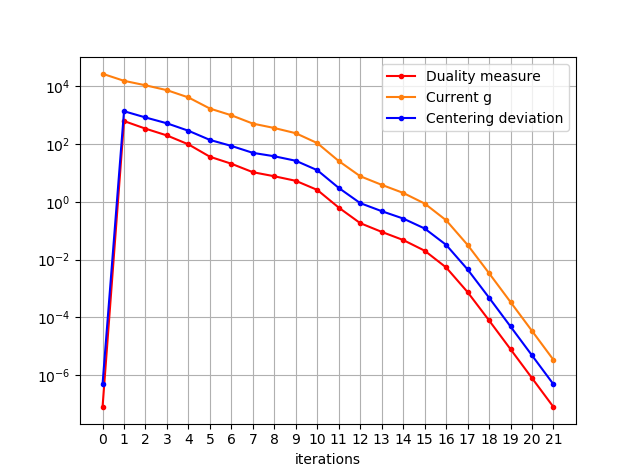
\includegraphics[width= 7 cm]{onb_aff1}} \qquad%
	\subfloat[Affine algorithm with MIP]{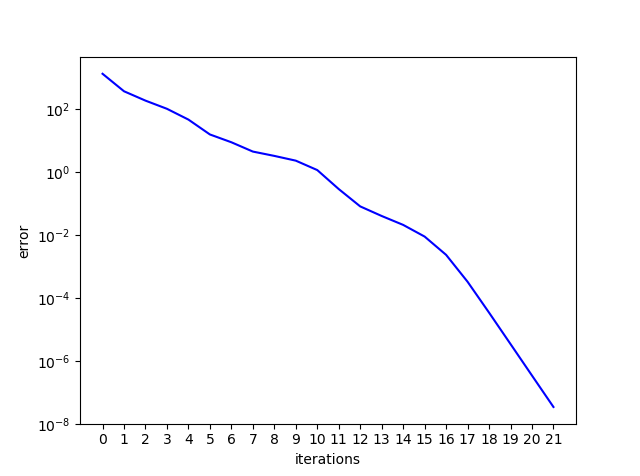
\includegraphics[width= 7 cm]{onb_aff2}}\\
	\subfloat[LPF 1 algorithm with MIP and with STP]{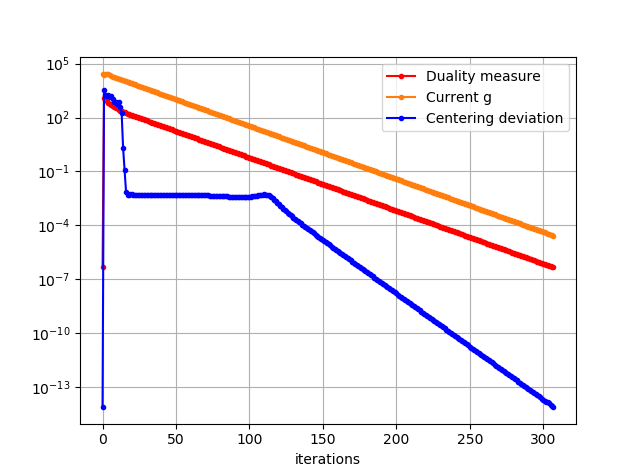
\includegraphics[width= 7 cm]{onb_LPF1}} \qquad%
	\subfloat[LPF 1 algorithm with MIP and with STP]{\includegraphics[width= 7 cm]{onb_LPF1b}}\\	
	\subfloat[LPF 2 algorithm with MIP and with STP]{\includegraphics[width= 7 cm]{onb_LPF2}} \qquad%
	\subfloat[LPF 2 algorithm with MIP and with STP]{\includegraphics[width= 7 cm]{onb_LPF2b}}\\
\end{figure}
\begin{figure}\caption{\label{figure:onb2}Execution of predictor-corrector IPMs on ONB model:}
	\subfloat[PC LPF algorithm with MIP]{\includegraphics[width= 7 cm]{onb_PCLPF}} \qquad%
	\subfloat[PC LPF algorithm with MIP]{\includegraphics[width= 7 cm]{onb_PCLPFb}}\\
	\subfloat[PC LPF algorithm with STP]{\includegraphics[width= 7 cm]{onb_PCLPF2}} \qquad%
	\subfloat[PC LPF algorithm with STP]{\includegraphics[width= 7 cm]{onb_PCLPF2b}}\\
	\subfloat[Mehrotra's algorithm with MIP]{\includegraphics[width= 7 cm]{onb_MER}} \qquad%
	\subfloat[Mehrotra's algorithm with MIP]{\includegraphics[width= 7 cm]{onb_MERb}}\\	\subfloat[Mehrotra's algorithm with STP1]{\includegraphics[width= 7 cm]{onb_MER2}} \qquad%
	\subfloat[Mehrotra's algorithm with STP1]{\includegraphics[width= 7 cm]{onb_MER2b}}\\
\end{figure}
\chapter{Conclusion}
The simplex method is the central computational element of Mathematical Programming Systems and this method works so well in practice but the computational process could break down for large values of $m$ and $n$ and even for reasonably sized problems.
We observed he Klee and Minty problem in which we can see the simplex method is an exponential-time algorithm; thus the algorithm does not have a polynomial bound. In the project we examine this case in order to motivate the centre of attention of the IPMs.
But it worths marking that all variables $(x, \lambda, s)$ computed by the latter change at each iteration and the linear algebra operations which are required to update them have to involve the complete matrix $A$. This makes a single iteration of the interior-point method significantly more expensive than that of the simplex method.\\

It is known that the generic predictor-corrector framework leads to a variety of interior-point methods for solving the linear problems and this research presents one. Our goal is to use the Mehrorta's technique in order to produce an acceleration of the performance of a general LPF method. The present thesis firstly introduces a framework of the IPMs algorithms in
the primal-dual class, focusing on the convergence analysis of the Affine and the LPF methods. The latter, imposing the iterates staying in a neighborhood,  obtains a potential advantage. In fact, while the neighborhood $\mathcal{N}_{-\infty}$ ensures that some products do not approach zero too early as with the pure Affine method, it does not prevent products from becoming too large with respect to the average. Next, the role of centrality of the predictor–corrector scheme in the implementation of interior-point methods is illustrated . \\
In order to gather these two potential techinques, we construct a Mehrotra-type method, the Predictor-Corrector LPF method, whose
behaviour we can understand and explain with computational tests.\\
The one unmistakable conclusion, with or without iterative refinement, is that the predictor-corrector algorithm is substantially superior to the pure primal-dual algorithm and
that this superiority grows with problem size and complexity, as we can note in Figure 4.3. We have performed some tests on four real
problems with fictitious data and the results indicate that Mehrotra's method takes
fewer iterations than the predictor-corrector LPF
method. Instead, the number of iterations required by this method appears similar to the
number of iterations taken by LPF 2.
Hence, it does not provide a complete picture of centrality of the iterate; anyway, if the centering parameter is left fixed, then the behavior of the
algorithm becames unstable.\\
In fact, the use of the predictor-corrector technique is advantageous in long-path following method: it leads to significant saving in the number of iterations. We believe that significant improvements to the algorithm can and will be made over time.
However, we personally were both gratified and somewhat surprised at how robust and
efficient this PC LPF code has proved to be, even when geometrically is not evident. \\
Besides, it is indicated an interesting
topic for the future research: you can opt for weel-suited the neighborood parameters to remedy such difficulties or investigate whether changing $\gamma$ PC LPF outperforms the Mehrtora's algorithm.\\
A further study could consist on the reduction of the parameter $\gamma$ in PC LPF in the Affine-scaling step, which has the effect of "opening" the cone, that is, expanding the neighborhood a little. 
%\begin{appendices}
\appendix
\chapter{The codes}	
 Let us present the codes I have implemented with Python's programming language for the analysis and the study of the algorithms.
 \section{Simplex method code}\label{app:A.1}
 \lstinputlisting[language=Python]{SimplexMethodIIphases.py}
 \section{Affine scaling method code}
 \lstinputlisting[language=Python]{AffineMethod.py}
 \section{LPF method codes}
 Long-Path Following method with centering parameter $\sigma^{1}$:
 \lstinputlisting[language=Python]{LPFMethod.py}
With centering parameter $\sigma^{2}$:
 \lstinputlisting[language=Python]{LPFMethod2.py}
Predictor-Corrector Long-Path Following method: 
 \lstinputlisting[language=Python]{LPFMethod_PC.py}
\section{MPC method code}
\lstinputlisting[language=Python]{MehrotraMethod.py}
\newpage
\section{Starting points codes}
 \lstinputlisting[language=Python]{starting_point.py}
 \lstinputlisting[language=Python]{starting_point2.py}
\section{Termination code}
 \lstinputlisting[language=Python]{term.py}
	\chapter{Newton's method}
	\section{}
	\textcolor{red}{NON SO SE AGGIUNGERE LA DESCRIZIONE DEL METODO DI NEWTON}\\
	Let $F \colon \mathbb{R}^{n} \to \mathbb{R}^{n}$ be a continuously differentiable function, with $F(x) = [F_{1}(x),\dots,F_{n}(x)] $. Consider the common problem to find a point $x^{*}\in\mathbb{R}^{n}$ for which:
\begin{equation*}
F(x^{*})=0.
\end{equation*}
Newton's method is an iterative method for solving this problem. One step of the method is defined as follows. Given any point $x\in\mathbb{R}^{n}$, it is computed a step direction $\Delta x$ for which $F(x + \Delta x)=0$. Obviously, for a nonlinear function $F$ it is not possible to find such a step direction. Hence, it is approximated by the first two terms of its Taylor's series expansion,
\begin{center}
	$F(x+\Delta x)\approx F(x) + F'(x)\Delta x$,
\end{center}
where
\begin{align*}
F'(x)= \begin{bmatrix}\frac{dF_{1}(x)}{dx_{1}}&\frac{dF_{1}(x)}{dx_{2}}&\dots&\frac{dF_{1}(x)}{dx_{n}}\\
\frac{dF_{2}(x)}{dx_{1}}&\frac{dF_{2}(x)}{dx_{2}}&\dots&\frac{dF_{2}(x)}{dx_{n}}\\
\vdots&\vdots&\dots&\vdots\\
\frac{dF_{n}(x)}{dx_{1}}&\frac{dF_{n}(x)}{dx_{2}}&\dots&\frac{dF_{n}(x)}{dx_{n}}\\
\end{bmatrix}.
\end{align*}
The approximation is linear in $\Delta x$. Hence, equating it to zero gives a linear system to solve for the step direction:
\begin{center}
	$F'(x)\Delta x = -F(x)$.
\end{center}
Given $\Delta x$, Newton's method updates the current solution $x$ by replacing it with $x+\Delta x$. The process continues until the current solution is approximately a root (i.e., $F(x)\approx0$). \\
The Newton’s method is very important to solve the linear system associated with the IPMs and it is applied in order to find a point on the central path $\mathcal{C}$, that is a vector $(x,\lambda, s)$ such that
 \begin{center}
	$\mathit{F}(x,\lambda,s)= \begin{bmatrix}
	A^{T}\lambda+s-c \\Ax-b \\XSe-\tau e
	\end{bmatrix}=0$, with $(x,s)\geq0$.
\end{center}The matrix of derivatives of $F$, the Jacobian $\mathit{J}$ is given by
 \begin{equation*}
 J(x,\lambda,s)=\begin{bmatrix}
 0&A^{T}&I \\A&0&0\\X&0&S
 \end{bmatrix}.
 \end{equation*}
With the matrix defined above the Newton direction $(\Delta x, \Delta \lambda, \Delta s)$ is computed but we see that a full step along this direction usually is not permissible, since it would violate the bound $(x,s)\geq 0 $. To avoid this difficulty, it is performed a line search along the Newton direction so that the new iterate is
\begin{center}
	$(x,\lambda,s)+\alpha (\Delta x, \Delta \lambda, \Delta s)$
\end{center}
for some line search parameter $\alpha\in(0,1]$, labelled as \textit{step length parameter}.

\begin{thebibliography}{9}
	
	% A
	\bibitem{MARE} Adler I., Monteiro R. D. C., Resende M. G. C., \emph{"A polynomial-time primal-dual affine scaling algorithm for linear and convex quadratic programming and its power serier extension."}, Math. of OR, 15, pp: 191-214, (1990).
	\bibitem{ADL} Adler I., Monteiro R. D. C., \emph{"Limiting behaviour of the affine scaling continuous trajectories for linear programming problems."}, Mathematical Programming, pp: 29-51, (1991).
	\bibitem{2} Andersen E. D., Ye Y.,  \emph{"Combining interior-point and pivoting algorithms for Linear Programming"}, (1996).
	\bibitem{ADL} Andersen E. D., Gondzio J., Mèszàros C., Xu X., \textit{"Implementation of interior point methods for large scale linear programming"}, Technical report, HEC,
    University of Ginevra, (1996).
    %
	% C
	%
	\bibitem{Carta}Cartis C., \emph{"Some disadvantages of a Mehrotra-type primal–dual corrector interior-point algorithm
	for linear programming"}, Technical report 04/27, Numerical Analysis Group, Computing Laboratory,
	Oxford University, (2004).
	\bibitem{Col}Colombo M, Gondzio J, \emph{"Further development of multiple centrality correctors for interior point
	methods"}, Computational optimization and applications, vol. 41, no. 3, pp. 277-305, (2008).

	\bibitem{SPS} D'Apuzzo M., De Simone V., di Serafino D., \emph{"Starting-point strategies for an infeassible potential reduction method"}, Springer-Verlag, D. Optim Lett, 4, pp: 131-146, (2010).
	\bibitem{DAN1}Dantzig, G. B., \emph{"Maximization of a linear function of variables subject to linear
	inequalities"}, Activity Analysis of Production and Allocation, pp: 339-347, (1947).
	\bibitem{1}Dantzig, G. B.,\emph{\;"Linear Programming and Extensions"}, Princeton University Press, Princeton, N.J., (1963).	
	\bibitem{DAN}Dantzig, G. B.,\emph{\;"Expected number of steps of the simplex method for a linear program with a convexity constraint"}, Technical Report SOL 80-3, Systems Optimization Laboratory, Department of Operations Research, Stanford University, Stanford, CA, (1980).
	\bibitem{FEM}Drayer W., Seabury S.,\emph{\;"Facilities Expansion Model"}, Interfaces, 5:2, part 2, pp: 104-109, (1975).
	%\bibitem{DAN} G. B. Dantzig, A. Orden, P. Wolfe, \emph{ Notes on linear programming: Part I- The generalized simplex method for
	%minimizing a linear form under linear inequality restrictions.} Pacific J Math pp: 183-195, (1955). 
	
	% G
	
	\bibitem{25y} Gondzio J, \textit{ "Interior Point Methods 25 years later"}, European Journal of Operational Research 218, Issue 3, pp. 587-601, (2011).	
	
% K
		\bibitem{ONB}Krajewski L. J., McKenzie P., Ritzman L. P.,\textit{ "Shift Scheduling in Banking Operations: A Case Application"}, Interfaces, 10:12, (1980).
		\bibitem{Kar} Karmarkar N. K.,\emph{ "A new polynomial-time algorithm for linear programming"}, Combinatorica, (1984).
		\bibitem{(Natural)} Kent B., Bare B. B., Field R. C., Bradley G. A., \textit{"Natural Resource Land Management Planning Using Large-Scale Linear Programs: The USDA Forest Service Experience with FORPLAN"}, OR, 39, pp. 13-27, (1991).
		\bibitem{Lem} Lemke C.E,\textit{ "The dual method of solving the linear programming problem."} Naval Research Logistics Quarterly, John Wiley and Sons, (1954).
		\bibitem{MINTY} Klee, V., Minty, G.,\emph{ "How good is the simplex algorithm?"} in O. Shisha, ed., ‘Inequalities–III’, Academic Press, New York, pp: 159–175, (1972).
		\bibitem{LNP}Luenberger David G., Yinyu Ye, \emph{"Linear and Nonlinear Programming"}, Springer Science+Business Media, 3, pp: 136-140, (2008).
		\bibitem{LMS} Lustig I. J., Marsten E., Shanno D. F.,\emph{ "Computational experience with a primal-dual interior point method for linear programming"}, Linear algebra and its applications, pp. 191-222, (1991).
		\bibitem{ComTeq} Maros I., \emph{"Computational Techniques of the Simplex Method"}, 1, Kluwer
		Academic Publishers, Boston, (2003).
		\bibitem{meg} Megiddo N., \emph{"Pathways to the optimal set in linear programming"}, in Progress in Mathematical Programming: Interior-Point and Related Methods, Springer-Verlag, New York, pp. 131-158, (1986).
	\bibitem{MER} Mehrotra S., \emph{ "On the implementation of a primal-dual interior point method"}, SIAM Journal on Optimization. 2, pp: 575-601, (1992).
	\bibitem{MUR} Mehrotra S., \emph{ Advanced Linear Programming: Computation and
	Practice. } McGraw-Hill New York, New York, (1981).
\bibitem{Mehr} Mehrotra S., \emph{"Generalized predictor-corrector methods and their performance"}, Technical Report 90-93, Department of Industrial Engineering and Management Sciences, Northwestern University, Evanston, Illinois, (1991).
		\bibitem{5}Mizuno S., Todd M.J., Y. Ye,\emph{\;On adaptive-step primal-dual interior-point algorithms for linear programming}, Math. of OR, vol. 18, pp. 964-981, (1993). 
	%	
	%N
	%
	\bibitem{W}Nocedal J., Wright J. S., \emph{\;"Numerical Optimization"}, Springer Series in OR, Springer, New York, (2006).

	\bibitem{Lexico2}  Charnes A., \emph{ "Optimality and degeneracy in linear programming"}, pp. 160-170, (1952). 

\bibitem{RR} Rardin Ronald L., \textit{"Optimization in operations reseasch"}, Pearson Education (US), 2, University of Arkansas, (2017).
\bibitem{rene}Renegar J., \textit{ "A Mathematical View of Interior-Point Methods in Convex Optimization"}, MPS/SIAM
Ser. Optim., SIAM, Philadelphia, 2001.

	%
	%T
	%
	\bibitem{Topia} Tapia, R., Zhang, Y., Saltzman, M., Weiser, A.,\emph{The Mehrotra predictor–corrector interior-point
	method as a perturbed composite Newton method}, SIAM J. Optim. 6, pp. 47–56, (1996).
\bibitem{ForSer} \emph{"Forest Service planning: accommodating uses, producing outputs, and sustaining ecosystems"}, Congress of the United States-Office of technology assessment.
\bibitem {VAN} Vanderbei J. Robert, \emph{\;"An interior point code for quadratic programming"}, Optim. Methods Software, 1, pp: 451-484, (1999). 
\bibitem {LP} Vanderbei J. Robert, \emph{\;"Linear programming:
Foundations and Extensions"}. Dept. of Operations Research and Financial Engineering
Princeton University, Springer Science + Business Media, (2001).
%
%W
%
\bibitem{SSM} Westerberg, C.-H., Bjorklund B., Hultman E., \emph{"An Application of Mixed Integer Programming in a Swedish Steel Mill" }, Interfaces, 7:2, pp: 39-43, (1977).
\bibitem {Wright} Wright J. Stephen, \emph{\;"Primal-Dual Interior Point Methods"}, SIAM: society for industrial and applied mathematics. Philadelphia, pag 134, (1997).
\bibitem{WWW}Wright M. H.,\textit{ “Interior point methods for constrained optimization”}, Acta Numerica, Cambridge Univ. Press, Cambridge, UK, pp. 341–407, (1992).
\bibitem{XY}Xiaojie Xu, Yinyu Ye, \emph{"A generalized homogeneous and self-dual algorithm for linear programming"}, Operations Research Letters, 17, pp. 181-190, (1995).
\bibitem{matlab}Zhang Y.,\textit{ "Solving large-scale linear programs by inteior point methods under
the Matlab enviroment"}, Optimization Methods and Software, 10, pp. 1-31, (1999).
\end{thebibliography}

\end{document}
